%% LyX 2.4.3 created this file.  For more info, see https://www.lyx.org/.
%% Do not edit unless you really know what you are doing.
\documentclass[12pt,american,english]{article}
\usepackage{lmodern}
\usepackage[LGR,T1]{fontenc}
\usepackage{textcomp}
\usepackage[latin9]{inputenc}
\usepackage{xcolor}
\usepackage{float}
\usepackage{amsmath}
\usepackage{amsthm}
\usepackage{amssymb}
\usepackage{graphicx}
\usepackage[letterpaper]{geometry}
\geometry{verbose,tmargin=2.5cm,bmargin=2.5cm,lmargin=2.5cm,rmargin=2.5cm}
\usepackage{setspace}
\usepackage[authoryear]{natbib}
\onehalfspacing

\makeatletter

%%%%%%%%%%%%%%%%%%%%%%%%%%%%%% LyX specific LaTeX commands.
\DeclareRobustCommand{\greektext}{%
  \fontencoding{LGR}\selectfont\def\encodingdefault{LGR}}
\DeclareRobustCommand{\textgreek}[1]{\leavevmode{\greektext #1}}


%%%%%%%%%%%%%%%%%%%%%%%%%%%%%% Textclass specific LaTeX commands.
\numberwithin{equation}{section}
\numberwithin{figure}{section}

%%%%%%%%%%%%%%%%%%%%%%%%%%%%%% User specified LaTeX commands.
\usepackage{fullpage}
\usepackage{subcaption}

\raggedbottom

%\usepackage{lineno}
%\linenumbers

%\usepackage[longnamesfirst]{natbib}

\usepackage{chngcntr}
\usepackage{booktabs}

\usepackage{array}
\newcommand{\PreserveBackslash}[1]{\let\temp=\\#1\let\\=\temp}
\newcolumntype{C}[1]{>{\PreserveBackslash\centering}p{#1}}
\newcolumntype{R}[1]{>{\PreserveBackslash\raggedleft}p{#1}}
\newcolumntype{L}[1]{>{\PreserveBackslash\raggedright}p{#1}}


\counterwithout{figure}{section}
\usepackage{color}
\usepackage{xcolor}
\usepackage{sectsty}
\usepackage{tikz}
\def\checkmark{\tikz\fill[scale=0.4](0,.35) -- (.25,0) -- (1,.7) -- (.25,.15) -- cycle;}

\usepackage{breakcites}
%\usepackage[authoryear,longnamesfirst]{natbib}
\usepackage[breaklinks=true]{hyperref}
\usepackage{setspace}
\onehalfspacing

\hypersetup{
    colorlinks,
    linkcolor={red!75!black},
    citecolor={blue!75!black},
}

\usepackage{geometry}
\geometry{
bottom=25mm,
top     = 25mm,
left     = 24mm,
right   = 24mm}

\setlength{\bibsep}{0pt plus 0.3ex}
\def\bibfont{\small}

\newcommand{\ccr}{\color{red}}
\newcommand{\ccb}{\color{blue}}
\renewcommand{\thetable}{\Roman{table}}

\sectionfont{\fontsize{15}{15}\selectfont}
\subsectionfont{\fontsize{14}{14}\selectfont}

%% CONTENTS FOR APPENDIX SEPARATELY %%
\usepackage{scrwfile}
\TOCclone[\contentsname]{toc}{atoc}
\newcommand\StartAppendixEntries{}
\AfterTOCHead[toc]{%
  \renewcommand\StartAppendixEntries{\value{tocdepth}=-10000\relax}%
}
\AfterTOCHead[atoc]{%
  \edef\maintocdepth{\the\value{tocdepth}}%
  \value{tocdepth}=-10000\relax%
  \renewcommand\StartAppendixEntries{\value{tocdepth}=\maintocdepth\relax}%
}
\newcommand*\appendixwithtoc{%
  %\cleardoublepage % starts on new page
  \appendix
  \addtocontents{toc}{\protect\StartAppendixEntries}
  \listofatoc
}

\makeatother

\usepackage{babel}
\title{\textbf{Expectation and Wealth Heterogeneity\\ in the Macroeconomy\thanks{Broer: PSE (tobias.broer@psemail.eu). Kohlhas: University of Oxford
(alexandre.kohlhas@economics.ox.ac.uk). Mitman: IIES, Stockholm University,
CEMFI (kurt.mitman@iies.su.se). Schlafmann: Copenhagen Business School
(ksc.fi@cbs.dk). For comments and useful suggestions, we thank Adrien
Auclert, Zhen Huo, Per Krusell, Tommaso Monacelli, Kristoffer Nimark,
Alessandra Peter, Morten Ravn, Matthew Rognlie, Kjetil Storesletten,
Laura Veldkamp, Gianluca Violante, Mirko Wiederholt, and seminar and
conference participants at various locations. A previous version of
this paper was circulated under the title ``Heterogeneous Information
Choice in General Equilibrium''. This research received financial
support from Ragnar Soderberg Stiftelsen and the European Research
Council (ERC) under the European Union's Horizon 2020 research and
innovation programme (Grant agreement No. 759482).\textbf{\textcolor{orange}{{}
}}Broer and Kohlhas thank the Institut Universitaire de France and
the John Felt Fund for financial support, respectively. Mitman gratefully
acknowledges the support of the Riksbankens Jubileumsfond, the Ministerio
de Ciencia, Innovacion y Universidades Grant IneqEx, and the Swedish
Research Council Project Grant 2023-01635. Schlafmann acknowledges
financial support from the Danish Finance Institute (DFI) and the
Center for Big Data in Finance (grant no. DNRF167).}}}
\date{July 2026}
\author{Tobias Broer\hspace{0.67cm}Alexandre Kohlhas\hspace{0.67cm}Kurt
Mitman\hspace{0.67cm}Kathrin Schlafmann}
\begin{document}
\maketitle
\begin{abstract}
\begin{singlespace}
We document systematic differences in macroeconomic expectations across
U.S. households and rationalize our findings with a theory of information
choice. We embed this theory into an incomplete-markets model with
aggregate risk. Our model is quantitatively consistent with the pattern
of expectation heterogeneity in the data. Compared with a full-information
counterpart, our model suggests substantially increased macroeconomic
volatility and inequality. We show through the example of an increase
in unemployment benefits that neglecting the information channel can
lead to misleading conclusions about the effects of macroeconomic
policies: by reducing information acquisition, improved unemployment
insurance raises macroeconomic volatility by an order of magnitude
more than in an otherwise identical model without information choice.\\\vspace{-0.26cm}
\end{singlespace}

\noindent JEL codes: D84, E21, E27, E63 \hspace{1.37cm}\\Keywords:
Expectations, heterogeneity, information\vspace{1.74cm}\thispagestyle{empty}\pagebreak{}
\end{abstract}

\section{Introduction\label{sec:introduction}}

\enlargethispage{\baselineskip}
Expectations have been part of the bedrock of modern macroeconomics
since the ``rational expectations revolution'' pioneered by Robert
E. Lucas, Jr., in the 1970s. The prevailing paradigm\textemdash the
full-information and rational expectations framework\textemdash posits
that all households, at all moments in time, have the same expectations
about the macroeconomy. Building on the work of \citet{muth1961rational}
and several others, \citet{mankiw2003disagreement} contrast this
prediction with survey data on expectations, showing instead the profound
dispersion of expectations that exists among households. Recent empirical
work has stressed that household expectations are not only heterogeneous
but also correlate systematically with household characteristics.
This creates systematic heterogeneity in both the level and accuracy
of expectations across the distribution of households (e.g., \citealp{carroll2003macroeconomic};
\citealp{lusardi2014economic}; \citealp{coibion2018formation}; \citealp{weber2022subjective}).
Given the importance of expectations to macroeconomics, it seems central
to have a theory of expectation formation that is consistent with
the data.

\emph{\setcounter{page}{1}}In this paper, we develop a theory of
information choice that we embed into a standard heterogeneous-agent
model with aggregate risk. Our main contribution is to provide the
first, to our knowledge, heterogeneous-agent model that allows for
the study of the macroeconomic consequences of systematic differences
in expectations. Our quantitative-theoretical framework can capture
both the rich differences in expectations, observed in the data, as
well as those that exist in wealth, income, and employment status.
Heterogeneity in income, wealth, and employment status on its own
significantly impacts the response of the economy to shocks (e.g.,
\citealp{KMP}; \citealp{kaplan2018microeconomic}). We use our framework\textemdash disciplined
by survey data\textemdash to assess the consequences of the expectation-wealth
nexus for understanding aggregate fluctuations and the distribution
of wealth. We then explore how the presence of heterogeneous expectations
can also modify the efficacy of macroeconomic policies.

We first provide new evidence on the heterogeneity in household expectations
using U.S. micro-level data. We show that in a leading household survey
(the New York Fed's Survey of Consumer Expectations) both the mean
and self-reported uncertainty of stated forecasts of key macroeconomic
variables differ substantially across households. Importantly, we
document that the accuracy of household expectations is systematically
related to household wealth: All else equal, wealthier households
have more accurate expectations; however, unlike the evidence in \citet{carroll2003macroeconomic}
and \citet{vissing2003perspectives}, this relationship is far from
clearly monotone\textemdash especially at the lower-end of the wealth
distribution, where the accuracy of household expectations appears
to decline with financial wealth.\footnote{A burgeoning literature has begun to document the various ways in
which household and firm expectations differ from one another and
within groups (e.g., \citealp{coibion2018formation}; \citealp{coibion2020inflation};
\citealp{reis2020people}; \citealp{andrade2022no}; and \citealp{mccauley}).
We contribute to this line of research by providing new evidence on
the systematic (non-monotone) relationship between the accuracy of
expectations and household wealth. Our estimates of the effects of
other characteristics (e.g., education and sex) are consistent with
those found in the literature (e.g., \citealp{lusardi2014economic}),
lending further support to our findings.}

Next, we embed dynamic information choice into an otherwise standard
business-cycle model with idiosyncratic risk and incomplete markets,
to explore households' heterogeneous incentives to acquire information.
In the model, households form expectations about future returns, wages,
and unemployment risk, to determine their optimal consumption-savings
choices, and acquire costly information about the state of the economy
to do so. The information that households can acquire approximates
the optimal signal that households would choose to design. The gains
to acquiring this information depend on household wealth, employment
status, and prior beliefs, leading to systematic heterogeneity in
expectations. 

While prior work has examined the financial and macroeconomic consequences
of costly information choices, it has primarily focused on once-and-for-all
information choices that are identical across time and decision-makers
(\citealp{grossman1980impossibility}; \citealp{sims2003implications};
\citealp{hellwig2009knowing}; \citealp{veldkamp2011information};
and \citealp{mackowiak2021rational}). In contrast, in our model,
households make \emph{dynamic information choices} that depend on
\emph{individual characteristics} at any point in time. We refer to
our synthesis of a heterogeneous-agent economy with a model of dynamic
information choice\textemdash and hence heterogeneous expectations\textemdash as
\texttt{HetExp}.

We show how to adapt results from the heterogeneous-agent literature
to provide a novel solution method for GE frameworks with dynamic
information choices and non-linear decision rules. Solving heterogeneous-agent
models with aggregate risk and non-linear decision rules is challenging.
Our framework adds a further layer of complexity by allowing for heterogeneity
also in expectations. We develop a tractable method to tackle these
challenges. In closely-related work, \citet{auclert2020micro} and
\citet{carroll2020sticky} analyze a heterogeneous-agent economy with
\emph{exogenous} information, based on \citet{mankiw2002sticky} and
\citet{carroll2003macroeconomic}, and (partially) linearized policy
rules. We document how the endogeneity of information and a fully
non-linear approach profoundly alter the macro consequences of incomplete
information.

Using our solution method, we calibrate our model framework to match
key features of U.S. macro and micro data. The model-generated distribution
of household expectations rationalizes the survey evidence. Heterogeneous
information choices\textemdash consistent with the data\textemdash naturally
arise from differences in wealth and employment status that are the
fundamental characteristics of heterogeneous-agent economies. To understand
households' heterogeneous incentives to acquire information\textemdash and
to highlight how they can profoundly shape macroeconomic outcomes\textemdash it
is instructive to understand households' savings decisions.

Consider first \emph{unemployed households, }who dissave to smooth
consumption\emph{.} The poorest\textemdash those at the borrowing
constraint for all states in the next period\textemdash have no benefit
from acquiring information. By contrast, unemployed households with
modest wealth have substantial benefits, as savings mistakes are costly
near the borrowing constraint. This is due to\textcolor{orange}{{} }the
curvature of both the utility and policy functions being high. As
wealth then increases, the value of information initially declines.
In this region, errors about future labor-market prospects and capital
returns push saving in opposite directions: Optimistic expectations
about the job-finding rate reduce precautionary savings, while expecting
a higher return on capital raise savings through intertemporal substitution.
In the middle of the distribution, these two effects partially offset
each other, temporarily lowering the value of information. At even
higher wealth levels, financial assets eventually comprise the bulk
of household resources and return risk, as a result, dominates, leading
to increasing information acquisition.

The value of information for \emph{employed households} is similar
to that of wealthy unemployed households: Employed households always
have (relatively) higher income, and thus cash-at-hand, compared to
unemployed, and separation rates are small. The value of additional
information about the state of the economy, as a result, starts low
and then rises with wealth.\enlargethispage{\baselineskip}

We show that such heterogeneity in information choices substantially
alters the equilibrium properties of the economy relative to the full-information
benchmark, in which all households have full information (and hence
common expectations) about the state of the economy.

On \emph{the} \emph{micro level}, heterogeneous information choices
feed back into wealth and income inequality, as differently informed
households make disparate savings choices. Indeed, the introduction
of heterogeneous information moderately exacerbates inequality. In
particular, poor households with incomplete information are unable
to exploit periods of good labor market prospects and high returns
to build up financial wealth; wealthy households with incomplete information
are likewise unable to effectively increase consumption and run down
savings when higher future returns increase their permanent income.
Both groups in response acquire information at higher rates than average,
yet still face substantial information frictions in equilibrium. The
introduction of heterogeneous incomplete information, as such, modestly
(but non-trivially) mitigates the lack of wealth inequality that exists
in standard frameworks.

On \emph{the macro level}, the presence of uninformed households leads
to an increase in business-cycle volatility, due to a stronger endogenous
propagation of shocks. Under full information, household savings are
procyclical; but as the aggregate capital stock rises in booms, the
return on savings falls, dampening the procyclicality of the savings
response. By contrast, uninformed households' expectations about returns
are sluggish to adjust, which makes household savings more procyclical
and the economy more volatile than under full information. This mechanism
is itself somewhat dampened by increased information acquisition,
due to the benefits of information about the economy being higher
when the economy is more volatile. In equilibrium, not all households
acquire information in every period, leading to 5-11 percent larger
fluctuations in consumption and output relative to the full-information
case.

Importantly, we show that these micro and macro results\textemdash and
the mechanisms behind them\textemdash extend to alternative versions
of our model that, for example, consider alternative information cost
structures and features of U.S. labor-income taxes. A prominent issue
with the Aiyagari-Bewley-Huggett-Imrohoroglu class of models that
we depart from is that it does not generate realistic wealth heterogeneity:
The data display significantly more skewness in wealth than the models.
Using an extension that builds on \citet{bayer2024shocks}, in which
a fixed share of wealthy entrepreneurs receive all pure profits in
the economy, we show that our results nevertheless carry over to a
framework that better matches the wealth distribution.

A key implication of our framework is that the interaction between
wealth and information choice alters the endogenous propagation of
aggregate shocks. Because households with different wealth levels
respond differently to information frictions, incomplete information
changes the cyclicality of savings and the persistence of the capital
stock, thereby amplifying business-cycle fluctuations. Policies that
reshape the wealth distribution therefore also reshape the economy\textquoteright s
information structure and can meaningfully modify aggregate dynamics
relative to standard full-information heterogeneous-agent models.
To demonstrate this, in the final part of the paper, we consider a
popular policy that directly affects the wealth-expectation nexus:
An increase in unemployment benefits.\footnote{Specifically, we consider an increase in the replacement rate from
40 to 50 percent of current wages.} This policy disproportionately affects the poor\textemdash one of
the two groups (along with the rich) that we find acquire information
at higher rates.\footnote{Notice that the policy reform considered here is stylized. Our focus
is mainly on illustrating how taking into account heterogeneity in
information choice can fundamentally alter, or even reverse, the consequences
of policies that affect the wealth distribution.}

The direct impact of the \emph{increase in unemployment benefits}
is to decrease household wealth, due to the reduced need for poorer
households to accumulate precautionary savings; its indirect effect
is to reduce information acquisition, as the reduction in income risk
from unemployment also decreases the incentive to acquire information
about the state of the economy. Because of the reduction in information
acquisition, business-cycle volatility rises by 4 percent. In contrast,
in the full-information case, the increase in unemployment benefits
has virtually no impact on aggregate volatility. Only the HetExp economy
generates additional business-cycle amplification through the information
channel. The effect of the increase in unemployment benefits on inequality
is similarly surprising: The Gini coefficient on wealth rises by 6
percent, nearly twice the increase under full information. As the
reduction in information acquisition is concentrated among the poor,
their reduction in savings is worsened by their inability to save
when future returns are high. The poor make larger errors precisely
when opportunities for wealth accumulation are greatest, lowering
their wealth. 

Overall, this policy experiment suggests that the consequences of
dynamic, heterogeneous information choices may substantially alter
the relative costs and benefits of macroeconomic policies. Our findings
thus imply a Lucas-style critique (\citealp{lucas1976econometric})
of policy evaluations in full-information heterogeneous-agent models:
Policies that reshape the wealth distribution also reshape an economy\textquoteright s
information structure and thereby modify economy-wide dynamics relative
to the predictions of standard full-information heterogeneous-agent
models.

Finally, three wider implications of our framework are worth noting.
First, in our analysis we for simplicity abstract from any behavioral
drivers of information choices (e.g., \citealp{bordalo2016stereotypes};
\citealp{bordalo2017memory}; and \citealp{gabaix2019behavioral}),
as well as any relationship between, for example, education, gender,
and household information (e.g., \citealp{lusardi2014economic} and
\citealp{reiche2025s}). Notwithstanding such alternative drivers,
we show that households' rational incentives to systematically acquire
different information, depending on their wealth and employment status,
fundamentally alter business-cycle dynamics and the consequences of
redistributive macroeconomic policies. We conjecture that behavioral
heuristics, salience effects, and other household drivers of information
choices would only increase the gap between the predictions of standard
models and those relevant for macroeconomic policy.

Second, our emphasis on households' rational information choices,
highlighting that wealth-poor households produce forecasts of close-to
commensurable accuracy to wealth-rich, connects with the small-scale
surveys in \citet{harrington1997other}, \citet{shipler2005working},
\citet{newman2009no}, \citet{morduch2017financial}, and others,
showing that poor and working-class households are often substantially
more aware of local conditions, prices, and opportunities, and devote
more mental resources to tracking economic conditions, than wealthier
households. We surmise that accounting for the full scale of such
effects would only lead to a richer relationship between household
informativeness and wealth than that detailed below. Our work is similarly
closely related to that in finance, documenting that informed, wealthier
investors often earn higher returns, which contributes to inequality
among traders (e.g., \citealp{peress2004wealth}; \citealp{kacperczyk2019investor};
and \citealp{mihet2019benefits}). Our work, in part, accounts for
a similar mechanism. 

Lastly, because of the complexity of computing rational expectations
equilibria in neoclassical heterogeneous-agent economies, several
authors have proposed dimensionality reduction methods (e.g., \citealp{moll2024trouble}).
Most notably, \citet{KS98} propose constraining households to only
form their expectations based on a limited set of moments. Through
this lens, our approach is to allow households themselves to decide
which variables (or moments) to use to forecast the future state of
the economy. In this sense, our framework presents a natural evolution
of the \citet{KS98} computational approach.

\section{Motivating Evidence\label{sec:motivating-evidence}}

We present new evidence on the relationship between household wealth
and the accuracy of household expectations. To do so, we use micro
data on household expectations from the \emph{Survey of Consumer Expectations
(SCE). }The SCE is a monthly panel of point and density forecasts
for several macroeconomic and financial variables. In addition, the
survey contains detailed data on household economic characteristics.\footnote{\citet{armantier2017overview} provide an overview of the construction
and scope of the Survey of Consumer Expectations, administered monthly
by the Federal Reserve Bank of New York (\citeauthor{data_sce}). } We link the monthly SCE expectation survey with the SCE's supplemental
survey of household finances, which includes detailed data on household
wealth and its composition. The merged SCE sample covers the period
2013M8-2020M1. Appendix \ref{sec:appendix-a} provides more information
on the sample construction.

We explore the relationship between the accuracy of household expectations
and their wealth. To do so, we first focus on household forecasts
of the one-year-ahead unemployment rate, as unemployment represents
the main source of income risk for many households.\textcolor{red}{{}
}As such, perceived unemployment risk is a main driver of households'
consumption and savings choices.\textcolor{red}{{} }We later include
unemployment into our structural framework. We define a respondent's
forecast error as the difference between the actual outcome and the
respondent's forecast. A negative error thus corresponds to an over-estimate
of the variable. The SCE ask respondents for the ``probability that
the unemployment rate is higher 12-months from now''. Unlike other
variables (e.g., inflation) for which we can observe realized outcomes,
the probability of unemployment rising is not objectively known. We
proxy the true-but-unobserved probability of rising unemployment with
the average probability computed from the \emph{Survey of Professional
Forecasters }(\citeauthor{data_spf})\emph{.} We make this choice
because professional forecasters often provide more accurate predictions
than even those from modern statistical and economic models.\footnote{See, for example, \citet{stark2010realistic}, \citet{faust2013forecasting},
and \citet{bhandari2019survey}. For interpretability reasons, we
also scale the value of unemployment forecast errors in the data with
the average proxied probability of rising unemployment, to approximate
the ``Brier score'' (Appendix \ref{sec:appendix-a}).} We later show how our results are robust to other proxies of the
probability of rising unemployment and extend to variables for which
realized outcomes are objectively known.
\begin{figure}
\caption{Unemployment Expectations Across the Wealth Distribution}
\label{fig-1-unemployment-errors}

\hspace{-0.65cm}
\includegraphics[scale=0.5]{_input/figure_1a_lhs}\hspace{0.22cm}
\includegraphics[scale=0.5]{_input/figure_1b_rhs}

\hspace{0.90cm}Panel (a): Relative Accuracy (SPF) \hspace{2.40cm}
Panel (b): Coefficient on Wealth (SPF)\vspace{0.00cm}

\hspace{-0.50cm}
\includegraphics[scale=0.5]{_input/figure_1c_lhs}\hspace{0.22cm}
\includegraphics[scale=0.5]{_input/figure_1d_rhs}

\hspace{0.90cm}Panel (c): Relative Accuracy (BVAR) \hspace{1.7cm}
Panel (d): Coefficient on Wealth (BVAR)\vspace{0.38cm}

{\footnotesize\emph{Note}}{\footnotesize : Panel (a) plots the difference
between the average one-year-ahead accuracy of unemployment forecasts
within wealth deciles/quintiles and the overall average taken across
all wealth levels. The true probability is proxied by the average
probability of rising unemployment from the SPF (Appendix \ref{app:data}).
Panel (b) plots the coefficient estimates on wealth from a regression
of the absolute value of individual errors on the wealth decile/quintile
the respondent belongs to, controlling for the age, education level,
labor market status, and sex of the respondent, as well as time fixed
effects. Estimates are relative to the wealthiest households, those
in the 80-100 percentile of the wealth distribution. Whisker-intervals
correspond to one-standard deviation robust confidence bounds (Table
\ref{tab:a1-unemployment-errors}). Panel (c) and (d) proxy the true
probability of rising unemployment with that from a standard forecasting
VAR (Online Appendix \ref{app:forecasting-VAR}). Sample: 2013M10-2020M1.}{\footnotesize\par}
\end{figure}

We begin by documenting a systematic correlation between household
forecast errors and household wealth. Panel (a) in Figure \ref{fig-1-unemployment-errors}
shows a marked, non-monotone relationship between household wealth
and the accuracy of household expectations in the raw data. All else
equal, wealthier households produce more accurate forecasts; however,
in contrast to the findings of \citet{carroll2003macroeconomic} and
\citet{vissing2003perspectives}, this pattern is only discernible
for households that are above the 20th percentile of the wealth distribution.
The poorest households\textendash\textendash those between the 0-10th
percentile of the wealth distribution\textendash\textendash produce
unemployment forecasts that are of comparable accuracy to those of
the wealthiest households. All else equal, this suggests that household
expectations are \emph{heterogeneous} across the wealth distribution.

The relationship in Panel (a) in Figure \ref{fig-1-unemployment-errors}
may be contaminated by idiosyncratic factors, such as labor-market
status, or aggregate shocks that can simultaneously affect household
wealth and the accuracy of expectations. To address this issue, Panel
(b) in Figure \ref{fig-1-unemployment-errors} plots the coefficient
estimates from a regression of the accuracy of individual expectations
on the household wealth-decile/quintile controlling for household
characteristics and time fixed effects. The regression coefficients
exhibit a similar non-monotonic relationship to that in the raw data.
All else equal, wealthier households make more accurate unemployment
forecasts; yet the accuracy of households in the bottom decile is
higher than those between the 20-40th percentile, although the difference
is not statistically significant at conventional levels. The magnitudes
are also meaningful: Considering a household in the 30th percentile
of the wealth distribution instead of the 90th percentile, all else
equal, decreases the accuracy of the household's expectations by around
9 percent. To benchmark the magnitude, having a university degree
is estimated to only increase accuracy by 7 percent (Table \ref{tab:a1-unemployment-errors}).\footnote{Our results on education are consistent with the findings of \citet{lusardi2014economic},
among others, who show that education, in part, through its impact
on financial literacy improves households' forecast accuracy. The
focus of our analysis is on the three-way relationship between wealth,
unemployment, and information, which is why we abstract from the influence
of education in what follows.} Crucially, Panel (c) and (d) in Figure \ref{fig-1-unemployment-errors}
show that our results also extend to cases where we proxy the probability
of rising unemployment with that computed from a standard forecasting
VAR (\citealp{christiano2005nominal}; \citealp{del2007fit}), while
Table \ref{tab:percentile-reg} in the Appendix shows that our results
further extend to the case in which we directly control for the percentile
rank of respondents in the wealth distribution. This illustrates the
robustness of our findings.

Clearly, the estimates in Figure \ref{fig-1-unemployment-errors}
cannot be interpreted as causal, as a household's wealth and the accuracy
of its expectations are determined jointly (e.g., Section \ref{sec:model}).
That said, the evidence is clearly at odds with the assumption of
common expectations embedded at the heart of the full-information
rational expectations framework, showing instead that the state of
household finances is closely tied to households' economic expectations.

\begin{figure}
\caption{Inflation and House Prices Expectations Across the Wealth Distribution}
\label{fig:2-inflation-houseprice-errors}\vspace{0.47cm}
\begin{centering}
Panel (a): Inflation Forecasts\vspace{-0.47cm}
\par\end{centering}

\includegraphics[scale=0.47]{_input/figure_2a_lhs}\hspace{0.22cm}
\includegraphics[scale=0.47]{_input/figure_2a_rhs}

\hspace{1.75cm} Actual Accuracy \hspace{4.95cm}Perceived Accuracy\vspace{0.29cm}\\
\begin{centering}
Panel (b): House Price Forecasts\vspace{-0.47cm}
\par\end{centering}

\includegraphics[scale=0.47]{_input/figure_2b_lhs}\hspace{0.22cm}
\includegraphics[scale=0.47]{_input/figure_2b_rhs}

\hspace{2.50cm} Actual Accuracy \hspace{5.30cm}Perceived Accuracy\vspace{0.47cm}

{\footnotesize\emph{Note}}{\footnotesize : Panels (a) to (d) show the
}{\footnotesize\emph{actual}}{\footnotesize{} and }{\footnotesize\emph{perceived}}{\footnotesize{}
accuracy of individual forecasts of one-year ahead CPI inflation and
the annual growth rate of U.S. house prices, respectively. All panels
plot estimates from regressions of individual (actual or perceived)
accuracy on the wealth decile/quintile the respondent belongs to,
controlling for the age, education level, labor market status, and
sex of the respondent, as well as time fixed effects. All estimates
are relative to the wealthiest households, those in the 80-100 percentile
of the wealth distribution. ``Actual accuracy'' corresponds to the
absolute value of individual forecast errors, while ``perceived accuracy''
corresponds to the interquartile range of the reported probability
distribution of the future outcome. Whisker-intervals are one-standard
deviation robust confidence bounds. Sample: 2013M10-2020M1.}{\footnotesize\par}
\end{figure}
We show that the systematic relationship between household wealth
and the accuracy of expectations extends to other macroeconomic variables.
We perform the same analysis for household forecasts of one-year-ahead
inflation and the growth rate of house prices. We use real-time data
to measure the realizations of inflation and house prices, to capture
the precise definition of the variable being forecasted. Figure \ref{fig:2-inflation-houseprice-errors}
summarizes the estimates. For both variables, Figure \ref{fig:2-inflation-houseprice-errors}
also includes the \emph{perceived} \emph{accuracy} of individual forecasts,
as measured by respondents' interquartile range of their stated probability
distribution of future outcomes. All estimates show that wealthier
households make more accurate forecasts and perceive themselves to
be less uncertain. Apart from inflation, all measures of uncertainty
are also higher for households near the 20-40th percentile of the
distribution than for poorest households.

Table \ref{tab:monotinicty-test} in the Appendix uses the ``worst-case''
Likelihood Ratio test developed by \citet{silvapulle2005constrained}
to explicitly test for the monotonicity of the regression coefficients
in Figure \ref{fig-1-unemployment-errors} and \ref{fig:2-inflation-houseprice-errors}.\footnote{Note that, because the regression coefficients are only set-identified
under the null hypothesis, the LR test corresponds to a ``worst-case
test''\textemdash it uses the coefficients most in line with the
null hypothesis. This makes any rejection of the null difficult, but
conversely also implies that any rejection provides strong evidence
against the null, which we interpret as evidence in favor of a humped-shaped
relationship.} As evident, 6 of the 8 tests reject the null hypothesis at the 10
percent level, providing instead evidence in favor of an inverse-u-shaped
relationship between wealth and the accuracy of expectations.\textcolor{orange}{{}
}Finally, in Appendix \ref{app:data} we perform additional robustness
exercises. There, we furthermore show that, compared to professional
forecasters, household expectations are more dispersed, less accurate,
and perceived to be more uncertain. We will later leverage these additional
moments to discipline our structural framework.

In summary, the results in this section provide evidence for systematic
heterogeneity in the accuracy of household expectations. The data
clearly reject the common-expectation assumption embedded in the full-information
rational expectations framework. Motivated by these findings, in the
next section, we extend a workhorse incomplete-markets economy to
allow for heterogeneity in the accuracy of household expectations.
We then proceed to quantify the impact of heterogeneous expectations
for positive and normative questions.

\section{Model Framework \label{sec:model}}

In this section, we describe a workhorse incomplete-markets model
with idiosyncratic and aggregate risk. The model extends the environment
in \citet{KS98} with a modified information structure. In particular,
we assume that every period households have the option to acquire
information about the state of the economy.

\subsection{Households}

The economy consists of a continuum of heterogeneous households $i\in[0,1]$,
whose preferences over streams of consumption and information are
described by the utility function:
\begin{equation}
\mathcal{U}_{i}=\mathbb{E}_{i0}\sum_{t=0}^{\infty}\beta^{t}\left[\frac{c_{it}^{1-\gamma}-1}{1-\gamma}-\kappa_{it}\left(\mathcal{I}_{it}\right)\right],\label{eq:utility}
\end{equation}
where $\mathbb{E}_{i0}\left[\cdot\right]\equiv\mathbb{E}\left[\cdot\mid\Omega_{i0}\right]$
denotes household $i$'s expectations conditional on its period-$0$
information set $\Omega_{i0}$, $\beta$ the effective discount factor
between two periods, $c_{it}$ non-durable consumption at time $t=\left\{ 0,1,2,\ldots\right\} $,
$\kappa_{it}$ the utility cost of acquiring information $\mathcal{I}_{it}$,
and $\gamma>0$. The effective discount factor $\beta=\rho b,$ where
$1-\rho\in(0,1)$ and $b\in(0,1)$ are the per-period probability
of death and the per-period discount factor, respectively.\footnote{Consistent with this, a fraction $1-\rho$ of households are born
every period with zero initial wealth.} The household\textquoteright s information set $\Omega_{it}$ accumulates
according to $\Omega_{it}=\left\{ \mathcal{I}_{it},\Omega_{it-1}\right\} $.\footnote{We will, ultimately, analyze the model beginning at $t>>0$, such
that the economy has settled into its ergodic distribution and any
effects of initial conditions have washed out.} The utility cost $\kappa_{it}$ follows a type-I extreme value distribution
with scale parameter $\alpha_{\kappa}$, and is i.i.d. across households,
time, and signals acquired. We introduce the extreme value shocks
to account for unobserved heterogeneity in the survey data and to
account for any utility costs of information processing.

Each household is endowed with $\bar{l}$ units of time, which it
supplies inelastically to the labor market. Labor productivity $\epsilon_{it}$
is stochastic and can take on two values, $\epsilon_{it}\in\left\{ 0,1\right\} $,
which we interpret as unemployment and employment, respectively. We
assume that $\epsilon_{it}$ follows a two-state, first-order Markov
process $\Pi_{z_{t+1},\epsilon_{it+1}\mid z_{t},\epsilon_{it}}$,
which depends on $\epsilon_{it}$ and aggregate total factor productivity
$z_{t}$ (described below). A household earns wage $w_{t}$ when employed
and receives unemployment benefits $\mu w_{t}$ when unemployed, where
the replacement rate equals $\mu\in(0,1$). We assume that households
cannot borrow but can save in physical capital $k_{it}$, whose net
return equals $r_{t}-\delta$, where $r_{t}$ denotes the stochastic
rental rate and $\delta\in(0,1)$ the depreciation rate of capital.
Households have access to perfect annuity markets.\footnote{The capital of the deceased is, thus, used to pay an extra proportional
return on capital of $\rho^{-1}$ .} 

In addition to the borrowing constraint and a non-negativity constraint
on consumption, household consumption-saving choices are restricted
by the per-period budget constraint: 
\begin{equation}
c_{it}+k_{it+1}=\left(1+r_{t}-\delta\right)\rho^{-1}k_{it}+\left(1-\tau_{t}\right)\left[\epsilon_{it}w_{t}\bar{l}+\left(1-\epsilon_{it}\right)\mu w_{t}\right]-\eta(\mathcal{I}_{it}),\label{eq:budget-constraint}
\end{equation}
where $\eta(\mathcal{I}_{it})$ denotes the resource cost of acquiring
$\mathcal{I}_{it}$, and $\tau_{t}$ is the tax rate on income. We
refer to the right-hand side of (\ref{eq:budget-constraint}) as a
household\textquoteright s \emph{cash-at-hand after choosing to acquire
information}, and denote it by $m_{it}$ in what follows. A household
maximizes utility (\ref{eq:utility}) subject to the budget constraint
(\ref{eq:budget-constraint}) and non-negativity constraints on $c_{it}$
and $k_{it+1}$.

\subsection{Technology and Markets}

The production sector consists of a representative competitive firm,
which maximizes profits. Output $Y_{t}$ is produced using a Cobb-Douglas
technology,
\begin{equation}
Y_{t}=z_{t}K_{t}^{\alpha}\left(L_{t}\bar{l}\right)^{1-\alpha},\label{eq:technology}
\end{equation}
where $K_{t}$ and $L_{t}$ denote aggregate capital and employment
in period $t$, respectively. Aggregate productivity $z_{t}$ is stochastic
and follows a first-order Markov process that takes two values, $z_{t}\in\left\{ z_{l},z_{h}\right\} $
with $z_{h}>z_{l}$. The firm rents capital and labor in competitive
markets, so that factor prices for labor $w_{t}$ and capital $r_{t}$
are given by their respective marginal products:
\begin{equation}
w_{t}=(1-\alpha)z_{t}\left(\frac{K_{t}}{\bar{l}L_{t}}\right)^{\alpha},\quad r_{t}=\alpha z_{t}\left(\frac{K_{t}}{\bar{l}L_{t}}\right)^{\alpha-1}.\label{eq:prices}
\end{equation}
Finally, we assume that the share of households in a given idiosyncratic
employment state only depends on the current value of productivity
$z_{t}$. Hence, the unemployment rate $u_{t}$ is a function only
of $z_{t}$, and thus only takes on two values, $u_{h}$ and $u_{l}$
with $u_{h}<u_{l}$.

\subsection{Government Policy\label{subsec:Government-Policy}}

In our baseline analysis, the government runs a balanced-budget unemployment
insurance scheme, such that $\tau_{t}=\frac{\mu u_{t}}{\bar{l}L_{t}}$.
Appendix \ref{app-sub-sec:acycl-taxes} and Section \ref{subsec:aggregate-implications}
discuss an alternative setup with acyclical income taxes. We consider
the response of the economy to changes in the replacement rate $\mu$
in Section \ref{sec:policy-experiment}.

\subsection{Timeline and Information Structure}

At the start of each period, idiosyncratic $\left(\epsilon_{it},\kappa_{it}\right)_{i}$
and aggregate shocks $(z_{t})$ realize. Firms rent capital and labor,
production takes place, and factor prices are determined. Households,
who do not observe the realization of aggregate shocks but know the
savings they brought into the period and their employment status,
then choose which signals $\mathcal{I}_{it}$ to acquire about the
current state of the economy from a maximum signal set $\mathcal{I}^{\text{max}}$.\footnote{We assume a household that is born in period $t$ inherits the information
set of its ``parent'' (i.e., the corresponding household that died
in period $t$). We experimented with different assumptions about
the informativeness of recently born households and found that it
makes little difference to our results below.} We assume that $\mathcal{I}^{\text{max}}$ does not contain sufficient
information for households to perfectly learn the current state of
the economy, but that it does include elements of the state-space
relevant for future prices (see below).\footnote{An alternative approach is to instead allow households to flexibly
design their optimal signal subject to a utility cost (e.g., \citealp{mackowiak2018dynamic}).
Such an optimal signal can, however, always be reduced to a signal
of some combination of state variables, which the above approach in
principle allows for. Furthermore, although the information-design
approach has several advantages, it is computationally intractable
for the non-linear, non-quadratic model that we study (see also Sections
\ref{subsec:recursive} and \ref{subsec:Remarks-on-Modeling}).} Finally, conditional on information choices and factor payments,
households make consumption and savings choices ($c_{it}$ and $k_{it+1}$,
respectively) and the period ends. 

\subsection{Recursive Formulation of the Household Problem\label{subsec:recursive}}

Given the timeline and informational assumptions, we develop a recursive
formulation of the household problem. Let $S=\left(\Gamma,z\right)$,
where $\Gamma$ denotes the cross-sectional distribution of capital
and employment status. We denote an individual household's first-order
belief about $S$ by $\mathcal{P}_{i}(S)$.\footnote{Not to be confused with the Powerset, $\mathcal{P}_{i}$ here has
a distribution with $\hat{\Gamma}_{i}$ and $\hat{z}_{i}$ as its
typical elements, representing household $i$'s first-order belief
about the mass of capital and employment status at some point, as
well as the household's beliefs about productivity, respectively.
$\mathcal{P}_{i}$ is hence a distribution over distributions.} Household $i$'s second-order belief about household $j\neq i$'s
belief is referred to as $\mathcal{P}_{ij}(S)$, and so on \emph{ad
infinitum}. Individual household beliefs are summarized by the object
$p_{i}$, which includes the infinite-set of household (higher-order)
beliefs. Let $\mathcal{P}$ denote the cross-sectional distribution
of all such beliefs.\footnote{More formally, we can describe $p_{i}=\left\{ \mathcal{P}_{i},\left(\mathcal{P}_{ij}\right)_{j\in\left[0,1\right]},...,\left(\mathcal{P}_{ij...k}\right)_{j,...,k\in\left[0,1\right]^{n-1}},...\right\} $,
while the cross-sectional distribution of such beliefs $\mathcal{P}=\left\{ \left(\mathcal{P}_{i}\right)_{i\in[0,1]},\left(\mathcal{P}_{ij}\right)_{i,j\in\left[0,1\right]^{2}},...,\left(\mathcal{P}_{ij...k}\right)_{i,j,...,k\in\left[0,1\right]^{n}},...\right\} $. } The \emph{aggregate state} of the economy can then be described by
$\Sigma=\left(S,\mathcal{P}\right)$, while the \emph{individual state}
variables at the stage in which consumption and savings choices are
made (\emph{Stage 2}) are described by $\sigma_{i,2}=\left(m_{i},\epsilon_{i},p_{i}\right)$,
where $m_{i}$ is household $i$'s cash-at-hand \emph{net} of information
costs. We denote next period's realization of variable $x$ by $x^{\prime}$
and previous period's realization by $x_{-1}$. The individual state
variables at the stage where information choices are made (\emph{Stage
1}) are $\sigma_{i,1}=\left(k_{i},\epsilon_{i},p_{i,-1}\right)$.
\smallskip

\noindent\emph{Stage 2:} At the end of the period, after making its
information choices, a household chooses consumption $c_{i}$ and
savings $k_{i}^{\prime}$ out of cash-at-hand net of information acquisition
costs: 
\begin{eqnarray}
\mathcal{W}\left(m_{i},\epsilon_{i},p_{i}\right) & = & \max_{c_{i},k_{i}^{\prime}\geq0}\frac{c_{i}^{1-\gamma}-1}{1-\gamma}+\beta\mathbb{E}\left[\mathcal{V}\left(k_{i}^{\prime},\epsilon_{i}^{\prime},p_{i}\right)\mid\Omega_{i}\right]\label{eq:vf-second-stage}\\
\text{subj.} & \text{to}\nonumber \\
c_{i}+k_{i}^{\prime} & = & m_{i}\nonumber 
\end{eqnarray}
where $\mathcal{W}(\sigma_{i,2})$ and $\mathcal{V}\left(\sigma_{i,1}\right)$
are a household's value functions \emph{after} and \emph{before} information
acquisition, respectively, and the expectation is taken using today's
updated information set $\Omega_{i}$. We let $g(\cdot)$ denote the
function that characterizes a household's savings choice (i.e., $k_{i}^{\prime}=g\left(\sigma_{i,2}\right))$,
while $h(\cdot)$ characterizes its consumption choice (i.e., $c_{i}=h\left(\sigma_{i,2}\right))$.
We assume that households rationally use the equilibrium law of motion
for the aggregate state, which we denote by $H$ (i.e., $\Sigma^{\prime}=H(\Sigma)$),
to form their prior expectation\textcolor{orange}{{} }about tomorrow's
state\textemdash and hence wealth $k_{i}^{\prime}$ embedded in $\sigma_{i,1}^{\prime}$\textemdash from
today's posterior beliefs. \emph{Stage 2} posterior beliefs $p_{i}$
are linked to \emph{Stage 1} priors $p_{i,-1}$ through Bayes' Rule
and the information choice $\mathcal{I}_{i}$ the household makes
in \emph{Stage 1}. \medskip

\noindent\emph{Stage 1:} At the beginning of the period, households
choose what information to acquire: 
\begin{eqnarray}
\mathcal{V}\left(k_{i},\epsilon_{i},p_{i,-1}\right) & = & \max_{\mathcal{I}_{i}\subseteq\left\{ \emptyset\cup\mathcal{I}^{\max}\right\} }\mathbb{E}\left[\mathcal{W}\left(m_{i},\epsilon_{i},p_{i}\left(\mathcal{I}_{i}\right)\right)-\kappa_{i}(\mathcal{I}_{i})\mid\Omega_{i,-1}\right]\label{eq:vf-initial-stage}\\
\text{subj.} & \text{to}\nonumber \\
m_{i} & = & \left[1+r\left(\Sigma\right)-\delta\right]\rho^{-1}k_{i}+\left(1-\tau\right)\left[\epsilon_{i}^ {}w\left(\Sigma\right)\bar{l}+\left(1-\epsilon_{i}\right)\mu w\left(\Sigma\right)\right]-\eta\left(\mathcal{I}_{i}\right).\nonumber 
\end{eqnarray}
Recall that information acquisition entails \emph{both} a utility
cost $\kappa\left(\mathcal{I}_{i}\right)$ and a resource cost $\eta\left(\mathcal{I}_{i}\right)$\textemdash and
that individual states and expectations themselves also depend on
the information choice $\mathcal{I}_{i}$. A household's expectation
in the first stage is computed using previous period's posterior belief
$p_{i,-1}$ (and hence information). We let $\iota\left(\cdot\right)$
denote the function that characterizes the household's optimal information
choice (i.e., $\mathcal{I}_{i}=\iota(\sigma_{i,1})$).

The assumption of type-I extreme value shocks for the utility cost
of information implies a parsimonious logistic choice function for
the probability of acquiring $\mathcal{I}_{i}\subseteq\left\{ \emptyset\cup\mathcal{I}^{\max}\right\} $:
\begin{equation}
\text{Prob}\left(\mathcal{I}_{i}\mid\sigma_{i,1}\right)=\frac{e^{\mathbb{E}\left[\alpha_{\kappa}\mathcal{W}\left(m_{i}\left(\mathcal{I}_{i}\right),\epsilon_{i},p_{i}\left(\mathcal{I}_{i}\right)\right)-\kappa_{i}(\mathcal{I}_{i})\mid\Omega_{i,-1}\right]}}{\sum_{\mathcal{\mathcal{\tilde{\mathcal{I}}}}\subseteq\left\{ \emptyset\cup\mathcal{I}^{\max}\right\} }e^{\mathbb{E}\left[\alpha_{\kappa}\mathcal{W}\left(m_{i}(\mathcal{\tilde{\mathcal{I}}}),\epsilon_{i,}p_{i}(\tilde{\mathcal{I}})\right)-\kappa_{i}(\tilde{\mathcal{I}})\mid\Omega_{i,-1}\right]}},\label{eq:prob-information-acq}
\end{equation}
where we suppress arguments other than $\mathcal{I}$ in the policy
functions, yielding the value function:
\begin{equation}
\mathcal{V}\left(\sigma_{i,1}\right)=\frac{\gamma_{E}}{\alpha_{\kappa}}+\frac{1}{\alpha_{\kappa}}\log\left(\sum_{\mathcal{\tilde{\mathcal{I}}}\subseteq\left\{ \emptyset\cup\mathcal{I}^{\max}\right\} }e^{\mathbb{E}\left[\alpha_{\kappa}\mathcal{W}\left(m_{i}(\mathcal{\tilde{\mathcal{I}}}),\epsilon_{i,}p_{i}(\tilde{\mathcal{I}})\right)-\kappa_{i}(\mathcal{\tilde{\mathcal{I}}})\mid\Omega_{i,-1}\right]}\right),\label{eq:vf-initial-after-info}
\end{equation}
where $\gamma_{E}$ is the Euler-Mascheroni constant (\citealp{mcfadden1973conditional}).

\subsection{Recursive Incomplete Information Competitive Equilibrium }

The definition of a \emph{Recursive Incomplete Information Competitive
Equilibrium} (RIICE) extends the standard definition of a Recursive
Competitive Equilibrium to the case with incomplete information: A
RIICE is a law of motion $H\left(\cdot\right)$, a pair of individual
value functions $\left\{ \mathcal{V}\left(\cdot\right),\mathcal{W}\left(\cdot\right)\right\} $,
policy functions $\left\{ g\left(\cdot\right),h\left(\cdot\right),\iota\left(\cdot\right),\right\} $,
as well as pricing functions $\left\{ r\left(\cdot\right),w\left(\cdot\right)\right\} $
such that: (i) $\left\{ \mathcal{V}\left(\cdot\right),\mathcal{W}\left(\cdot\right),g\left(\cdot\right),h\left(\cdot\right),\iota\left(\cdot\right)\right\} $
solve the household's optimization problem (i.e., Equations \ref{eq:vf-second-stage}-\ref{eq:vf-initial-stage})
given $H\left(\cdot\right)$; (ii) $r\left(\cdot\right)$ and $w\left(\cdot\right)$
satisfy firm maximization (i.e. Equation \ref{eq:prices}), (iii)
$H\left(\cdot\right)$ is generated by policy functions $g\left(\cdot\right)$,
$h\left(\cdot\right)$, and $\iota\left(\cdot\right),$ the Markov
process $\Pi_{z^{\prime},\epsilon^{\prime}|z,\varepsilon}$ , as well
as Bayes' Rule, using the information contained in $\left(\mathcal{I}_{i}\right)_{i}$
and current beliefs described in $\mathcal{P}$;\footnote{For example, we can construct the part of $H(\cdot)$ that pertains
to the marginal distribution of capital, $H_{k}\left(\cdot\right)$,
conditional on employment states and productivity, as follows. For
all measurable sets \foreignlanguage{american}{$\Delta k$:
\[
H_{k}\left(\Sigma\right)\left(\Delta k,\epsilon,z\right)=\sum_{\tilde{\epsilon}}\Pi_{\epsilon,z\mid\tilde{\epsilon},\tilde{z}}\cdot\int\mathbf{1}\left\{ g\left[m\left(k,\tilde{\epsilon};\Sigma\right),\tilde{\epsilon},p\right]\in\Delta k\right\} \cdot d\Phi\left(k,\tilde{\epsilon},p\right),
\]
where $\Phi(\cdot)$ denotes the joint cross-sectional distribution
of $\left(k,\epsilon,p\right)$.}} and (iv) market-clearing conditions hold for capital and goods markets
(e.g., for the goods market: $Y(\Sigma)+(1-\delta)K=\int\left(g(\sigma_{i,2})+h(\sigma_{i,2})+\eta\left[\iota\left(\sigma_{i,1}\right)\right]\right)di$).\footnote{Notice that the information cost $\eta\left(\mathcal{I}\right)$ is
paid in terms of the numéraire. Thus, the goods-market clearing condition
accounts for total information expenditures, $\int\eta\left(\mathcal{I}_{i}\right)di$.
\citet{baley2025data} discuss the different assumptions possible
for information costs (i.e., whether costs are paid in goods, labor,
or capital).}

\subsection{Remarks on Modeling Assumptions\label{subsec:Remarks-on-Modeling}}

The above recursive formulation helps clarify the nature of the two-sided
relationship between wealth and information that exists in our model.
On the one hand, a household's capital holdings and employment status,
in addition to its prior expectation, help determine the extent of
the household's information acquisition at the first stage of any
period (Equation \ref{eq:vf-initial-stage}). Yet, on the other hand,
a household's information choice also helps determine the household's
consumption-savings choice in the second stage, through its expectations,
and hence the household's future wealth level (Equation \ref{eq:vf-second-stage}).
This two-sided interaction, which we label the \emph{expectation-wealth
nexus}, will be central for the aggregate consequences of the accuracy-wealth
relationship documented in the data (Section \ref{sec:motivating-evidence}).

The recursive formulation further illustrates that our framework falls
within the broader class of ``noisy rational expectations'' models.
For example, although households are uncertain about the current state
of the economy, they rationally use the law of motion to form their
expectations about future productivity conditional on current information\textemdash and
hence the likelihood of, for instance, future information purchases.
As such, our framework is closely related to the work on ``costly
information acquisition'' within rational expectations frameworks
(e.g., \citealp{grossman1980impossibility}; \citealp{veldkamp2011information})
and its extension to ``rational inattention'' (e.g., \citealp{sims2003implications};
\citealp{mackowiak2021rational}). This literature has primarily restricted
itself to studying the implications of once-and-for-all information
choices that are identical across time and decision-makers. The contribution
of our framework, in this context, is to highlight the macroeconomic
consequences of \emph{dynamic, heterogeneous information choices}.\footnote{In our framework, we deliberately abstract from the ``non-instrumental
value'' of information and focus only on the consequences that information
has on utility through improving decision-making. \citet{brunnermeier2005optimal}
and \citet{caplin2019wishful}, among others, consider the consumption-saving
biases that arise when households engage in ``wishful thinking'',
in which expectations maximize average felicity, optimally balancing
the benefit of optimism against the costs of worse decision-making.}

Finally, notice that our benchmark model allows for both a resource
cost of information $\eta\left(\mathcal{I}_{i}\right)$ (Equation
\ref{eq:vf-initial-stage}) as well as a utility cost $\kappa_{i}(\mathcal{I}_{i})$
(Equation \ref{eq:vf-initial-stage}). The former captures the physical
costs associated with the acquisition of information, while the latter
captures the (cognitive) utility costs associated with its processing
(e.g., \citealp{veldkamp2011information}), in addition to accounting
for unobserved heterogeneity in the survey data.\footnote{\citet{veldkamp2011information} discusses how a resource cost of
information, for example, also captures the costs associated with
``getting advice from experts'' or out-sourcing decisions. \textcolor{blue}{Boccanfuso
and Neri} (\textcolor{blue}{2025}) document how a random utility component
to attention choices are necessary to match expectations in the SCE.} Crucially, the latter, for example, also captures the utility costs
associated with the processing of market-based information (see below
for further discussion). Our calibrated framework in Section \ref{sec:quantitative-results}
highlights the distinctive footprint that each of these information
costs has at the aggregate level.

\section{Solution Method and Calibration\label{sec:solution-and-calibration}}

In this section, we first outline our procedure for computing RIICE
equilibria. Our description here is deliberately non-technical. We
include it in the main text because our description is intimately
linked to the three-way relationship between information choices,
consumption-savings decisions, and the macroeconomy that is at the
heart of our analysis\textemdash and because it illustrates the underlying
methodology behind our framework. We then proceed to discuss the specification
of the information structure and the calibration of the model. 

\subsection{Computational Strategy}

The endogenous aggregate state variables of our economy, $\Gamma$
and $\mathcal{P}$, are infinite-dimensional objects. Even the \emph{full-information}
version of our incomplete-markets economy therefore presents a computational
challenge, because of the high dimensionality of $\Gamma$ (the endogenous
state variable of that model). Our \emph{incomplete-information} framework
has a \emph{double-infinity problem}\textemdash the additional complexity
arising from the entire set of (higher-order) beliefs $\mathcal{P}$
in principle mattering for equilibrium dynamics, depending on the
specification of $\mathcal{I}^{\text{max}}$.

The standard strategy for computing incomplete-markets models \emph{without}
incomplete information involves approximating the distribution $\Gamma$
with a finite set of moments ${\mathbf{m}}\equiv(m_{1},m_{2},\cdots,m_{n})$
(\citealp{KS98}). Accurately forecasting those moments enables households
to forecast future prices, which are necessary for solving the household
problem. One interpretation of the Krusell-Smith solution method is
one of ``boundedly rational'' expectations, as households only keep
track of a limited set of moments of the distribution. Importantly,
in this solution method, the information that households use to base
their expectations on is \emph{exogenously} \emph{predetermined} by
the researcher\textemdash containing productivity $z$ and the moments
in $\mathbf{m}$. By contrast, in our model, households \emph{optimally
choose} the information on which to form their ''boundedly rational''
expectations. Thus, one can view our model as a natural extension
of the Krusell-Smith approach to study incomplete-markets models with
aggregate risk, since we provide a micro-foundation for the boundedly-rational
solution based on costly information choice. In particular, the Krusell-Smith
solution can be seen as the special case in which the cost of information
is zero, and $\mathcal{I}_{it}=\mathcal{I}_{t}^{\max}=\{z_{t},\mathbf{m}_{t}\}$
for all $i$ and $t$, as a consequence.

In addition to predetermined information, notice that the Krusell-Smith
approach also imposes \emph{common knowledge} over both $z$ and $\mathbf{m}_{t}$,
as all households form expectations using the same information. Our
framework, by contrast, relaxes the common knowledge assumption by
allowing for heterogeneous information choices.\footnote{Both our framework and the Krusell-Smith framework assume common knowledge
over the underlying structure of the economy\textemdash in particular,
the law of motion $H\left(\cdot\right)$. Thus, if households knew
the current state of the economy, they would correctly forecast tomorrow's
state. That is why the Krusell-Smith solution can be seen as a special
case of our equilibrium concept when the cost of information is zero.} The RIICE framework, as a result, allows for the study of the three-way
interaction between incomplete common knowledge, aggregate dynamics,
and inequality that we focus on below\textemdash in contrast to Krusell-Smith.

Our computational strategy can be summarized as follows: Households
form priors over the contemporaneous realization of productivity $z$
and over a set of moments of $\Gamma$ given by $\mathbf{m}$. Given
those priors, using Bayes' Rule and the equilibrium law of motion
$H\left(\cdot\right)$, households form expectations about the future
path of wages and the return on capital, necessary to solve their
maximization problem. Households then choose what information to acquire
about any combination of productivity $z$ and the moments in $\mathbf{m}$,
which we include in $\mathcal{I}^{\max}$. If all households acquire
information about all elements in $\mathcal{I}^{\max}=\{z,\mathbf{m}\}$
in every period, our equilibrium coincides with the equilibrium concept
from \citet{KS98}.\footnote{Our assumption that households know the law of motion $H\left(\cdot\right)$
and use it to form expectations is in line with a large literature
on noisy rational expectations, going back to at least \citet{lucas1972expectations}.
In all of this work, agents observe signals about unobserved fundamentals,
characterizing the state of the economy, but crucially know the mapping
between the signals they observe and the underlying fundamentals,
as well as all other equilibrium relationships (e.g., \citealp{woodford2001imperfect};
\citealp{sims2003implications}; \citealp{lorenzoni2009theory}; \citealp{mackowiak2009optimal};
\citealp{coibion2012can,coibion2015information}; and \citealp{Angeletos_2021}
among others). This allows us to focus on the implications of uncertainty
about the state of the economy and not conflate any effects with those
that also arise from uncertainty about the structure of the economy.}

\subsection{The Specification of Moments}

For the set of moments households can choose between, we follow \citet{KS98}
and consider only the first moment of the cross-sectional distribution
of capital, $\mathbf{m}=\int g\left(\sigma_{i,2}\right)d\sigma_{i,2}=K_{t}$.
Even with this restricted set, the model in principle suffers from
the problem of \textquotedblright \emph{infinite regress of expectations}\textquotedblright ,
described in e.g., \citet{townsend1983forecasting}, which is induced
by the public observation of an endogenous market-outcome. To solve
this problem, we exploit a feature of Krusell-Smith-like economies:
The sequence of shocks $\left\{ z_{s}\right\} _{s=0}^{t}$ alone allows
for extremely accurate predictions about the future capital stock
$K_{t+1}$ (\citealp{DENHAAN20101}). We therefore set $\mathcal{I}^{\text{max}}=\left\{ z_{t}\right\} $,
so that households simply decide each period whether or not to acquire
information about the exogenous value of productivity $z_{t}$. Importantly,
we check \emph{ex post} that this assumption allows households to
form accurate posteriors about $K_{t}$, and thereby make accurate
predictions about future wages and rates of returns (Appendix \ref{app:model-fit}). 

A main result in the literature on optimal signal design is that optimal
signals can be reduced to signals about (some combination of) state
variables (e.g., \citealp{mackowiak2018dynamic}). Because the history
of aggregate productivity $z_{t}$ accurately approximates the relevant
state variables for prices in our economy (Appendix \ref{app:model-fit}),
our assumption can be viewed as allowing households to choose to observe
elements of the optimal signal.\footnote{We thank Mirko Wiederholt for this comment.}
Finally, in previous work (\citealp{BKKS_2}), we have shown that
the utility benefits of acquiring information about the capital stock
$K_{t}$ (or equivalent past productivity) conditional on current
productivity, $z_{t}$, assuming a Markov process for $z_{t}$, are
small\textemdash in the order of \$3-30 at 2020 prices.

\subsection{Approximated Problem and Equilibrium}

Given our assumptions, we can state the approximated household problem
that households solve: Households enter the period with capital $k_{i}$,
their employment status $\epsilon_{i},$ their prior over whether
the economy is in the high productivity state $p_{i,-1}^{z}\equiv\text{Prob}\left(z=z_{h}\mid\Omega_{i,-1}\right)$,
and their prior over the capital stock $p_{i,-1}^{K}$. Households
then choose whether to observe contemporaneous productivity $z$.\footnote{For computational tractability, we assume households have a point
prior on capital, $p_{i}^{K\prime}=\mathbb{E}\left[\tilde{H}(z,p_{i}^{K})|\Omega_{i}\right]$.
Appendix \ref{app-subsec-wealthy} shows that our results are extremely
similar when households internalize uncertainty in their forecasts
about capital, analogous to the findings in \citet{DENHAAN20101}
and \citet{BKKS_2}.} In line with the above notation, let $\tilde{\sigma}_{i,2}\equiv\left(m_{i},\epsilon_{i},p_{i}^{z},p_{i}^{K}\right)$
and $\tilde{\sigma}_{i,1}\equiv\left(k_{i},\epsilon_{i},p_{i,-1}^{z},p_{i,-1}^{K}\right)$.
The two-stage optimization problem can then be stated as:\smallskip

\noindent\emph{Stage 2: Consumption-savings choice}
\begin{eqnarray}
\tilde{\mathcal{W}}\left(\tilde{\sigma}_{i,2}\right) & = & \max_{c_{i},k_{i}^{\prime}\geq0}\frac{c_{i}^{1-\gamma}-1}{1-\gamma}+\beta\mathbb{E}\left[\tilde{\mathcal{V}}\left(\tilde{\sigma}_{i,1}^{\prime}\right)\mid p_{i}^{z},p_{i}^{K\prime}\right]\label{eq:approx-problem-2}\\
\textrm{{subj.}} & \textrm{{to}}\nonumber \\
c_{i}+k_{i}^{\prime} & = & m_{i}\nonumber \\
K^{\prime} & = & \tilde{H}(z,K)\nonumber \\
p_{i}^{z} & = & \text{Prob}\left(z=z_{h}\mid\Omega_{i}\right),\quad p_{i}^{K\prime}=\mathbb{E}\left[\tilde{H}(z,p_{i}^{K})|\Omega_{i}\right].\nonumber 
\end{eqnarray}

\noindent\emph{Stage 1: Information choice} 
\begin{eqnarray}
\tilde{\mathcal{V}}\left(\tilde{\sigma}_{i,1}\right) & = & \max_{\mathcal{I}_{i}\in\{\emptyset,z\}}\mathbb{E}\left[\tilde{\mathcal{W}}\left(\tilde{\sigma}_{i,2}\right)-\kappa_{i}(\mathcal{I}_{i})\mid p_{i,-1}^{z},p_{i}^{K}\right]\label{eq:approx-problem-1}\\
\textrm{{subj.}} & \textrm{{to}}\nonumber \\
m_{i} & = & \left[1+r\left(z,K\right)-\delta\right]\rho^{-1}k_{i}+\left(1-\tau\right)\left[\epsilon_{i}w\left(z,K\right)\bar{l}+\left(1-\epsilon_{i}\right)\mu w\left(z,K\right)\right]-\eta\left(\mathcal{I}_{i}\right)\nonumber 
\end{eqnarray}
Notice that $\tilde{H}(z,K)$ in Equation (\ref{eq:approx-problem-2})
is the law of motion for the aggregate capital stock, which replaces
$H\left(\cdot\right)$ as the aggregate law of motion in the approximated
problem. Thus, in addition to their individual cash-at-hand and employment
status, households forecast the probability of being in the high-productivity
state and the aggregate capital stock. Households update their priors
after their information acquisition choice using Bayes' rule. Consistent
with the notation above, we let $\tilde{h}\left(\cdot\right)$, $\tilde{g}\left(\cdot\right)$,
and $\tilde{\iota}\left(\cdot\right)$ denote the policy functions
for consumption, capital, and information, respectively (i.e., $c_{i}=\tilde{h}\left(\tilde{\sigma}_{i,2}\right)$,
$k_{i}^{\prime}=\tilde{g}\left(\tilde{\sigma}_{i,2}\right)$, and
$\mathcal{I}_{i}=\tilde{\iota}\left(\tilde{\sigma}_{i,1}\right)$).
The aggregate state variable is denoted by $\tilde{\Sigma}=\left(z,K\right)$
in what follows. 

We provide a brief overview of the numerical procedure that we use
to solve for the approximated RIICE equilibrium. To solve for the
equilibrium fixed point, we use an iterative procedure: First, we
postulate a law of motion $\tilde{H}\left(\cdot\right)$ for the aggregate
state variables. As in \citet{KS98}, we assume a log-linear relationship
between $K^{\prime}$ and $K$, whose coefficients depend on the (boom
or bust) realization of $z$. Second, we solve the household's two-stage
problem in (\ref{eq:approx-problem-1}) and (\ref{eq:approx-problem-2})
conditional on $\tilde{H}\left(\cdot\right)$. We use Equation (\ref{eq:prob-information-acq})
and the EGM-algorithm from \citet{carroll2006method} to solve for
the policy functions and value function iteration to solve the value
functions. Third, using the resulting individual decision rules, we
simulate a large number of households for a long number of periods.
From this simulation, we then calculate a time-series for $K$, and
estimate a new law of motion $\tilde{H}^{\prime}\left(\cdot\right)$
(i.e., new log-linear relationships). We iterate until convergence
on $\tilde{H}\left(\cdot\right)$.

\subsection{Calibration}

The aim of our calibration exercise is to ensure that the model can
account for salient business-cycle and cross-sectional facts, as well
as capture the rich heterogeneity in household expectations documented
in Section \ref{sec:motivating-evidence}. We assume that a model
period corresponds to one quarter.

\paragraph{Externally Calibrated Parameters: }

We choose standard parameters for the capital share $\alpha$ (0.36)
and the depreciation rate $\delta$ (0.025). Following \citet{KMP},
we calibrate the structure of aggregate and idiosyncratic risk to
capture key features of the unemployment and job-finding rates in
the post-World War II U.S. economy. We define \textquotedblright booms\textquotedblright{}
and \textquotedblright busts\textquotedblright{} based on the observed
unemployment dynamics, as those more closely align to our model framework
than traditional NBER-dated recessions. We define a boom as a period
with a below-trend unemployment rate.\footnote{We use an HP filter with smoothing parameter $\lambda$ equal to 14.400
to construct the trend in the unemployment rate from monthly unemployment
data (\citealp{ravn2002adjusting}).} The productivity variable $z_{t}$ is calibrated to match the difference
in average U.S. total factor productivity during booms and busts.
We estimate the persistence of booms and busts to be $0.88$ and $0.82$,
respectively, and the ratio of productivity values $z_{h}/z_{l}=1.027$.
The individual transition probabilities in labor productivity $\epsilon_{it}$
are set to match U.S. labor market transitions calculated from the
Current Population Survey. We choose an unemployment rate in booms
and busts equal to 6 and 10 percent, respectively. Monthly job-finding
rates are set to match unemployment-to-employment flows in the CPS
(\citealp{data_cps}), and are equal to $55$ and $45$ percent in
boom and busts, respectively. The remaining transition probabilities
are then pinned down by the requirement that  unemployment depends
only on current productivity $z_{t}$. Finally, we set the UI replacement
rate $\mu$ to $0.40$.

\paragraph{Internally Calibrated Parameters:}

We calibrate the discount factor $b=0.987$ and the probability of
death $1-\rho=0.005$ to generate\textcolor{blue}{{} }a quarterly capital-output
ratio of 10 (\citealp{carroll2017distribution}) and to be consistent
with an expected work-life of 45 years. We calibrate the degree of
relative risk aversion $\gamma$ and the information cost parameters
$\alpha_{\kappa}$ and $\eta$ to quantitatively capture key features
of the micro-data on expectations discussed in Section \ref{sec:motivating-evidence}.
We set $\gamma=5$ and the monetary cost per signal equal to\textcolor{blue}{{}
}$\eta=0.0028$ (equivalent roughly to $0.1$ percent of quarterly
pre-tax wages) to match our empirical finding that forecast accuracy
increases in wealth for richer households (Section \ref{subsec:results-accuracy}).\footnote{The benefit of additional information for wealthy households arises
mainly from improved predictions about the future rate of return on
capital. Yet when relative risk aversion is close to one, income and
substitution effects largely cancel one another, and wealthy households
do not value those improved predictions.} We set the scale parameter $\alpha_{\kappa}$ equal to $1/15\times10^{-4}$
to capture the dispersion in unemployment expectations observed in
the SCE (even for households with similar observable characteristics).
To check how household expectations compare to those in the SCE, we
concentrate on expectations of future unemployment. Table \ref{tab:exp-data-1}
compares the accuracy and standard deviation of households' one-year
ahead unemployment rate errors in the model and the data. Recall that
the SCE elicits expectations of future unemployment in the form of
the \textquotedblleft percent chance that 12-months from now the unemployment
rate in the U.S. will be higher than it is now\textquotedblright .
For households in the model, we therefore compute the difference between
a household\textquoteright s perceived probability conditional on
its current information $\text{Prob}(u_{t+4}>u_{t}|\Omega_{it})$
and the true probability $\text{Prob}(u_{t+4}>u_{t}|z_{t})$, which
depends on current productivity $z_{t}$. We then compare the resulting
errors with the corresponding errors in the survey data. Table \ref{tab:exp-data-1}
shows that the dispersion of errors is somewhat larger in the data,
but that overall the model replicates both the accuracy and volatility
of expectation errors in the data well. Table \ref{app:calibration-param}
in the Appendix summarizes the parameters. 
\begin{table}
\caption{Unemployment Expectations: Model vs. Data}

\label{tab:exp-data-1}\textcolor{black}{\vspace{-0.22cm}}

\textcolor{black}{\def\sym#1{\ifmmode^{#1}\else\(^{#1}\)\fi}

\begin{tabular*}{\textwidth}{@{\extracolsep{\fill}} l c c }
\hline\hline
 &  Mean Abs. Error   & Std. Dev. of Abs. Error  \\
\hline
Survey of Consumer Expectations         &  1.28   & 0.68  \\
[1em]Model Simulated Data                   & 1.27   &  0.52 \\
\hline
\hline
\end{tabular*}

}

\vspace{0.22cm}

{\footnotesize\emph{Note}}{\footnotesize : The table shows the mean
and standard deviation of the absolute value of errors in the probability
that the unemployment rate four quarters ahead is higher than at time
$t$. The table compares the simulated moments from the calibrated
model to those from the Survey of Consumer Expectations (see Section
\ref{sec:motivating-evidence} for a description). For interpretability
reasons, we scale the absolute value of unemployment errors in the
model and in the data with the average true probability of rising
unemployment, proxied in the data with average probability of rising
unemployment from the Survey of Professional Forecasters (Section
\ref{sec:motivating-evidence}).}{\footnotesize\par}
\end{table}


\section{Quantitative Results\label{sec:quantitative-results}}

In order to understand the drivers and consequences of households'
information choices, we proceed in four steps. First, we analyze how
different information choices affect household savings decision\textemdash the
intertemporal decision variable in the model. Second, we characterize
how household information choices depend on individual state variables,
such as wealth. Third, we combine the insights from the first two
steps to show how the interaction between information and savings
choices allows us to match the micro data on expectations. Finally,
we explain the impact of the wealth-expectations nexus on aggregate
dynamics and inequality, and show that our results carry over to several
alternative versions of our benchmark model.

\subsection{Savings Choices and Information\label{subsec:savings-information-nexus}}

We start by describing how information affects households' savings
choices, $k_{i}^{\prime}$. These micro-level effects are central
for understanding the aggregate amplification we later document. In
the model, households save to smooth consumption in the face of volatile
income and to intertemporally substitute consumption in response to
movements in the interest rate. The state of the economy that households
can acquire information about affects these both through \emph{exogenous}
\emph{fluctuations} in productivity and employment, and through \emph{endogenous}
\emph{fluctuations} in capital\textemdash all of which matter for
households' labor income and future rates of return. 

\begin{figure}[t!]

\caption{Savings Choices Compared to Full-information Model}
\label{fig:3-savings-choices}

\begin{subfigure}[t]{0.48\textwidth}
  \centering
  \caption{Distribution of Savings Differences}
  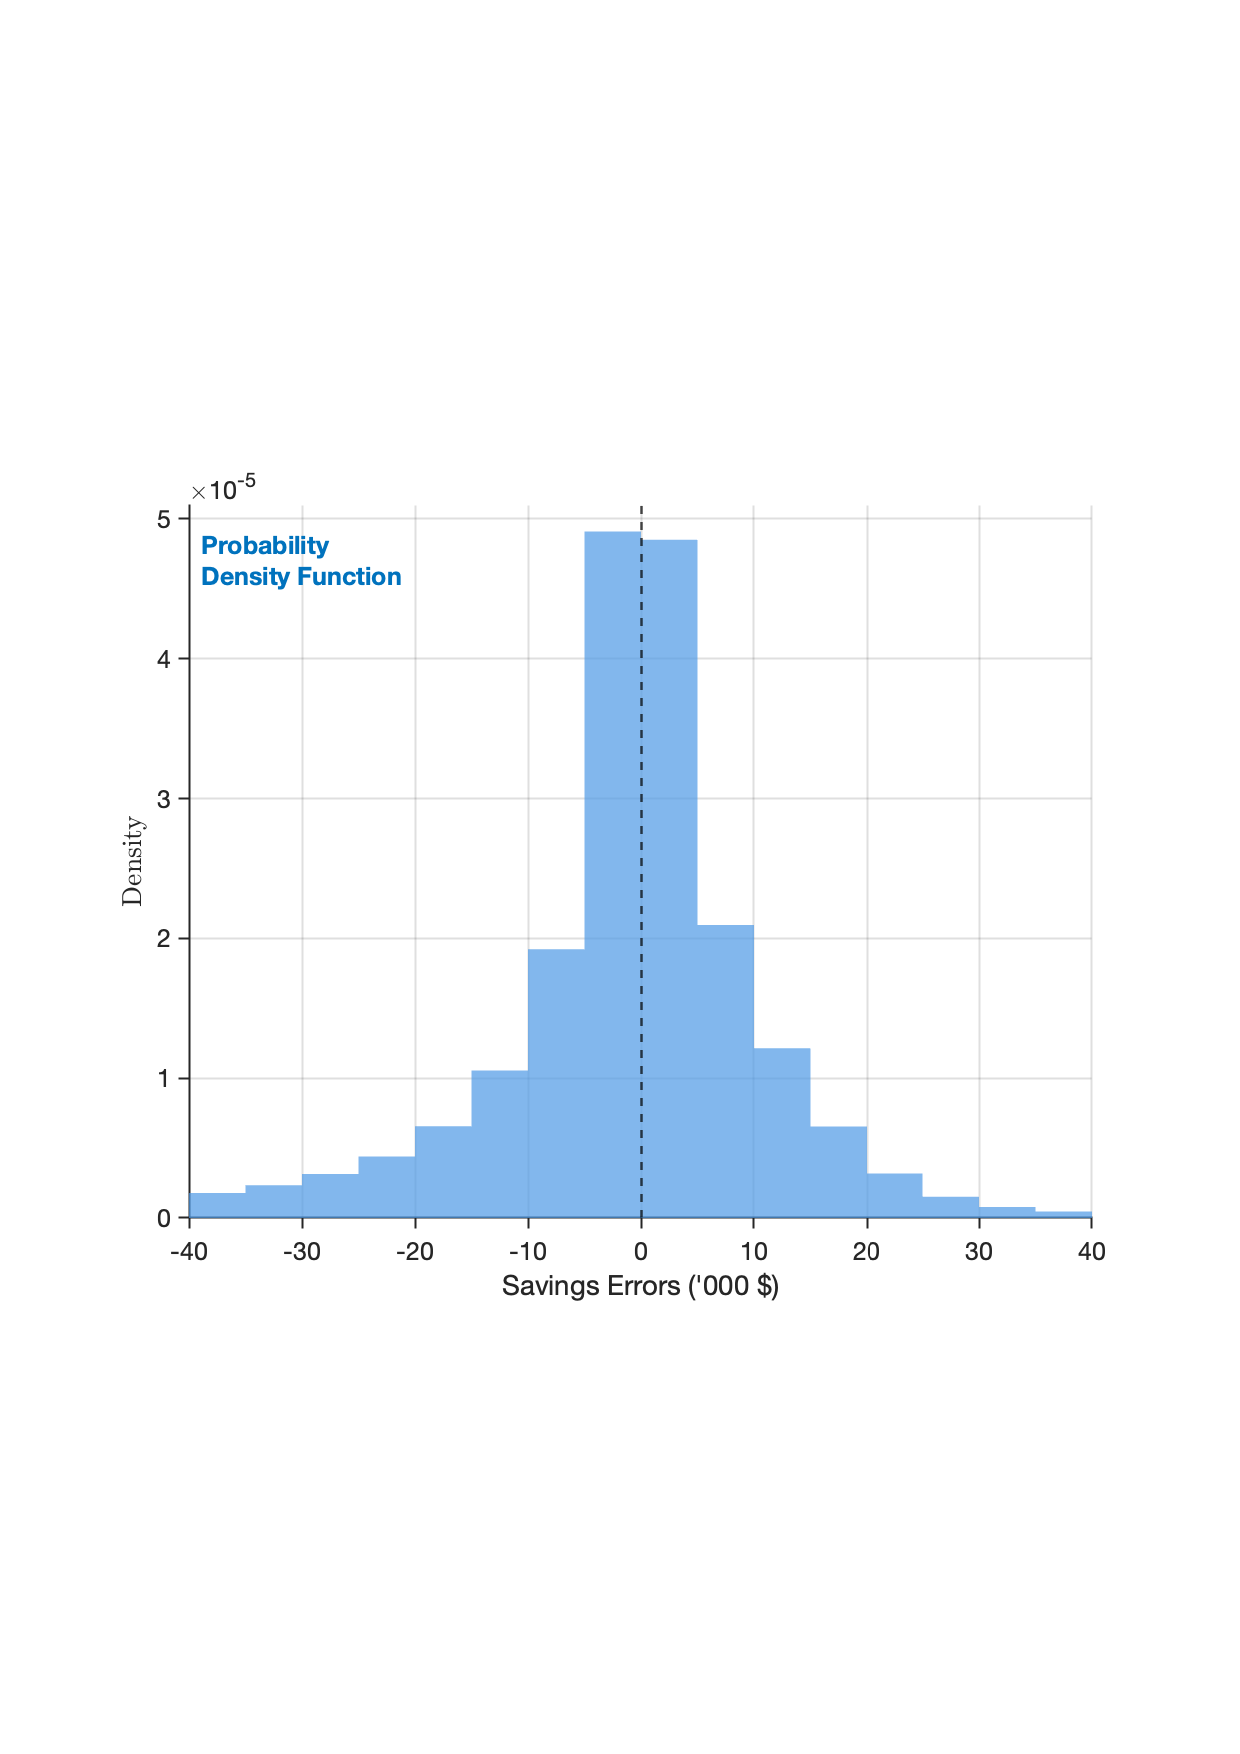
\includegraphics[width=\linewidth,trim=29 160 29 224,clip]{_input/figure_3a.pdf}
% \includegraphics[width=\linewidth,trim=29 160 29 224,clip]{_input/savings_errors.pdf}
\end{subfigure}\hfill
\begin{subfigure}[t]{0.48\textwidth}
  \centering
  \caption{Informed vs. Full Information}
 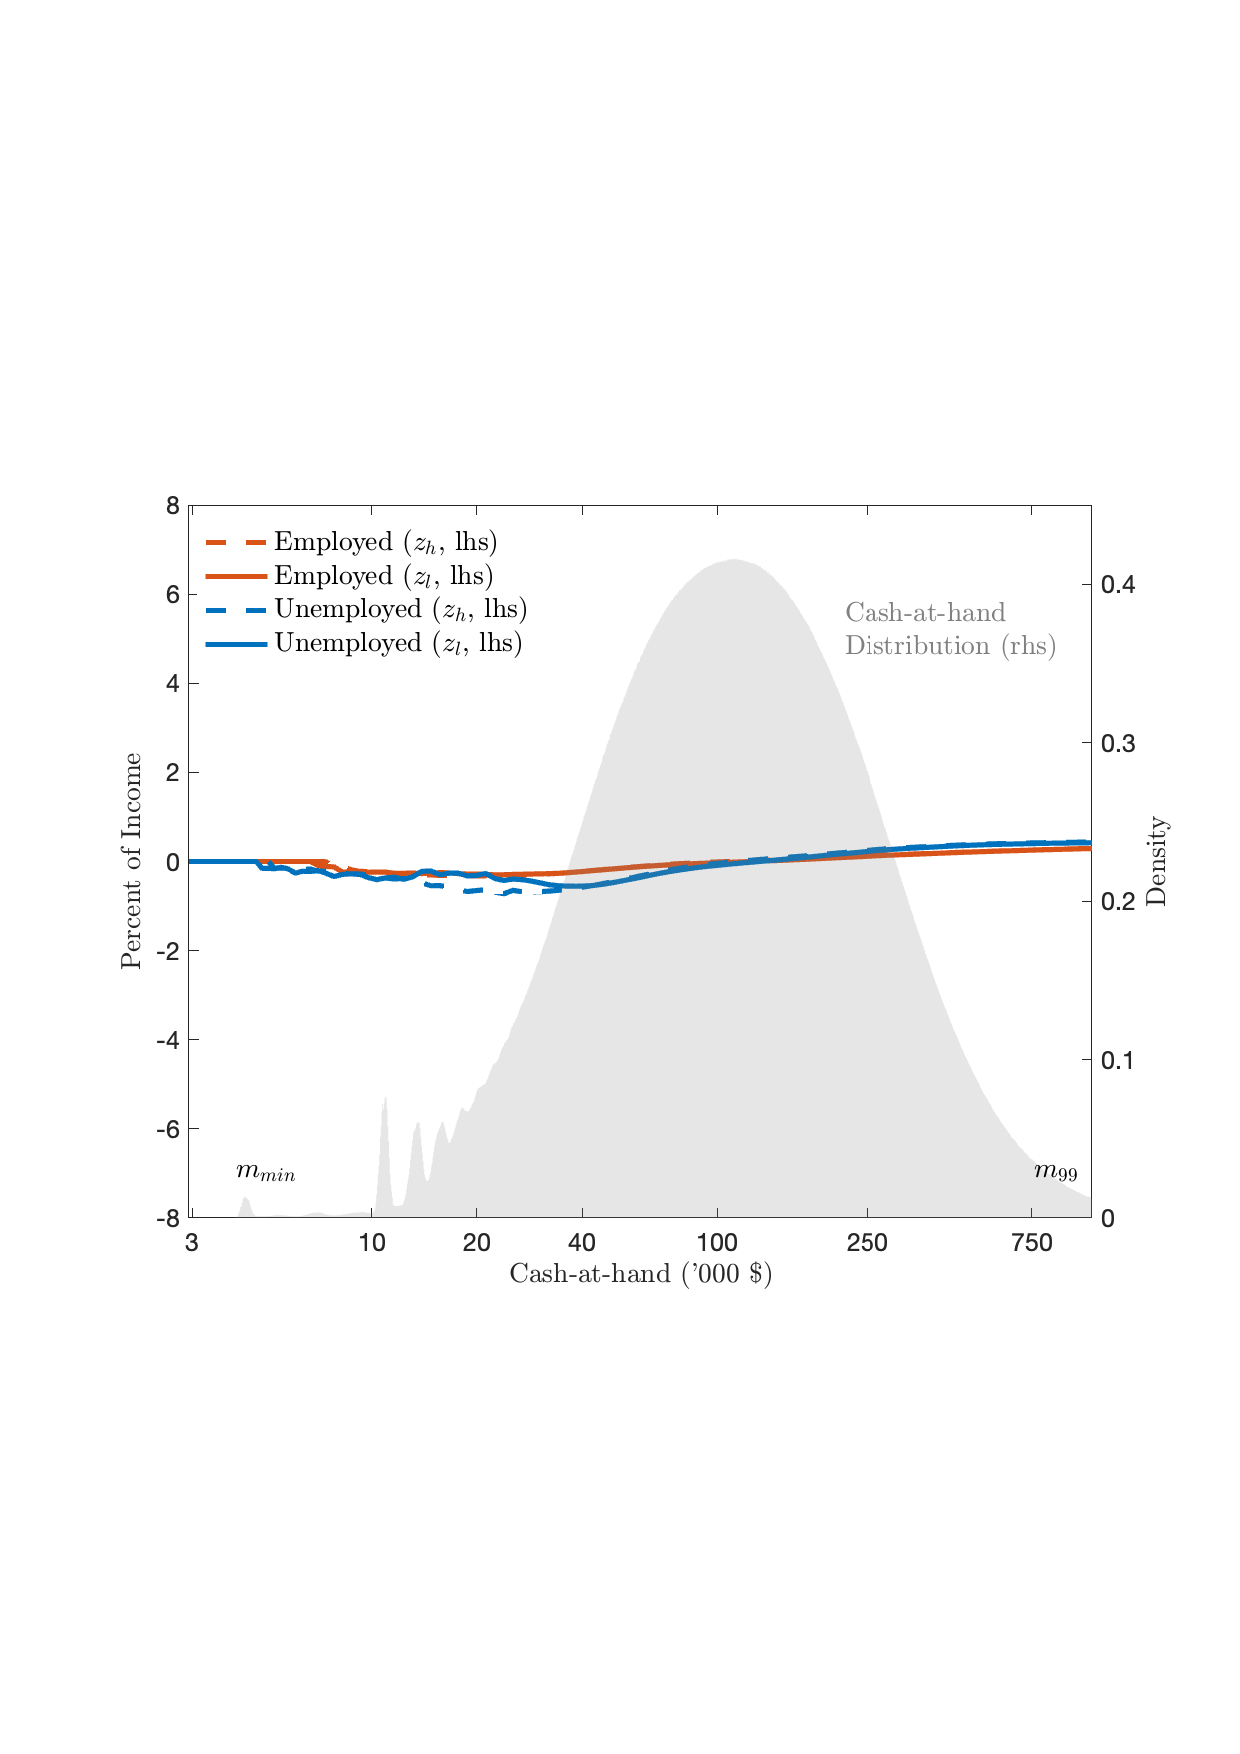
\includegraphics[width=\linewidth,trim=29 160 29 224,clip]{_input/figure_3b.pdf}
% \includegraphics[width=\linewidth,trim=29 160 29 224,clip]{_input/savingsfullinformation.pdf}
\end{subfigure}

\vspace{-0.47cm}
\footnotesize

%\justifying
\noindent                {\protect\footnotesize \textit{Note:}  The figure compares  savings choices in the benchmark economy to those from the full-information  economy. Panel (a) shows the distribution of savings differences   using the same sequence of aggregate and idiosyncratic shocks.  Panel (b) plots the differences between the savings choice of "an informed household", who has just acquired information about $z$, in our benchmark ecoonmy and the savings choice of a household in the full-information economy as a percent of household income.  We plot this difference in a recession (solid lines, $z=z_l$) and a boom (dashed lines, $z=z_h$) for both an unemployed (in blue) and employed (in red) household, and overlay the distribution of cash-at-hand in the benchmark economy in gray. The figure also depictes the minimum of cash-at-hand ($m_{min}$) and its 99th percentile value ($m_{99}$). We plot savings differences as a function of cash-at-hand and use 2020 values of U.S. household income to convert into USD (\$) amounts. 
}
\end{figure}
\vspace{0.29cm}

\noindent\textbf{Comparison to Full-information.} Panel (a) in Figure
\ref{fig:3-savings-choices} plots the distribution of differences
in savings choices between the benchmark (heterogeneous incomplete-information)
HetExp economy and the economy in which all households exogenously
acquire information every period. We refer to this counterfactual
economy as the ``full-information economy''; it corresponds to the
workhorse full-information (Krusell-Smith) analog of our benchmark
economy.\footnote{Notice that we assume households still pay the resource and utility
cost of information acquisition in the full-information economy. Section
\ref{sub-sect-ext:cost} compares our results to the case in which
households do not pay these costs.{\footnotesize{} We re-calibrate the
discount factor to target the same $K/Y-$ratio as in our benchmark
economy and use the same sequence of aggregate and idiosyncratic shocks
in all model simulations. }} For comparison, on average, only around 10 percent of households
choose to acquire information in any given period in our benchmark
economy.\footnote{{\footnotesize The probabilities of information acquisition in the
benchmark economy are 0.122 and 0.097 for the unemployed and employed,
respectively. The average rate of unemployment is 7.6 percent.}}\textbf{ }We plot differences in quarterly savings choices based on
a simulated panel of households with identical idiosyncratic and aggregate
shocks across the two economies. Differences in savings choices are
often considerable\textemdash approx. 20\% of them exceed \$20,000
in absolute value. Clearly, such large differences have the potential
to matter for macroeconomic outcomes, and arise due to a combination
of the presence of incomplete information and its implications for
the dynamics of the economy. 

Panel (b) in Figure \ref{fig:3-savings-choices} starts to break down
the drivers of these differences by showing that they are \emph{not}
\emph{driven by the behavior of informed households}. It does so by
comparing the savings choices of a household who has just acquired
information in our benchmark model and a household in the full-information
version of the model. We plot differences in savings choices (``benchmark
informed minus full-information'') as a function of a household's
cash-at-hand and assume both households have the same expectation
about capital. The figure further conditions on the same perceived
law-of-motion (from the benchmark economy), which embodies the aggregate
dynamics of the economy. Any differences in savings choices thus result
from informed households in the benchmark economy \emph{anticipating
being uninformed in the future}. The resulting differences are small\textemdash often
less than 1\% of income\textemdash and do not vary much with either
the individual employment state (employed or unemployed) or the aggregate
state of the economy (boom $z_{h}$ or bust $z_{l}$). The large differences
in Panel (a) clearly do not arise from differences in informed households'
savings choices.

\begin{figure}[t!]

\caption{Savings Choices, Information, and Wealth}
\label{fig:4-savings-choices}

\begin{subfigure}[t]{0.48\textwidth}
  \centering
  \caption{Informed vs. Uninformed}
    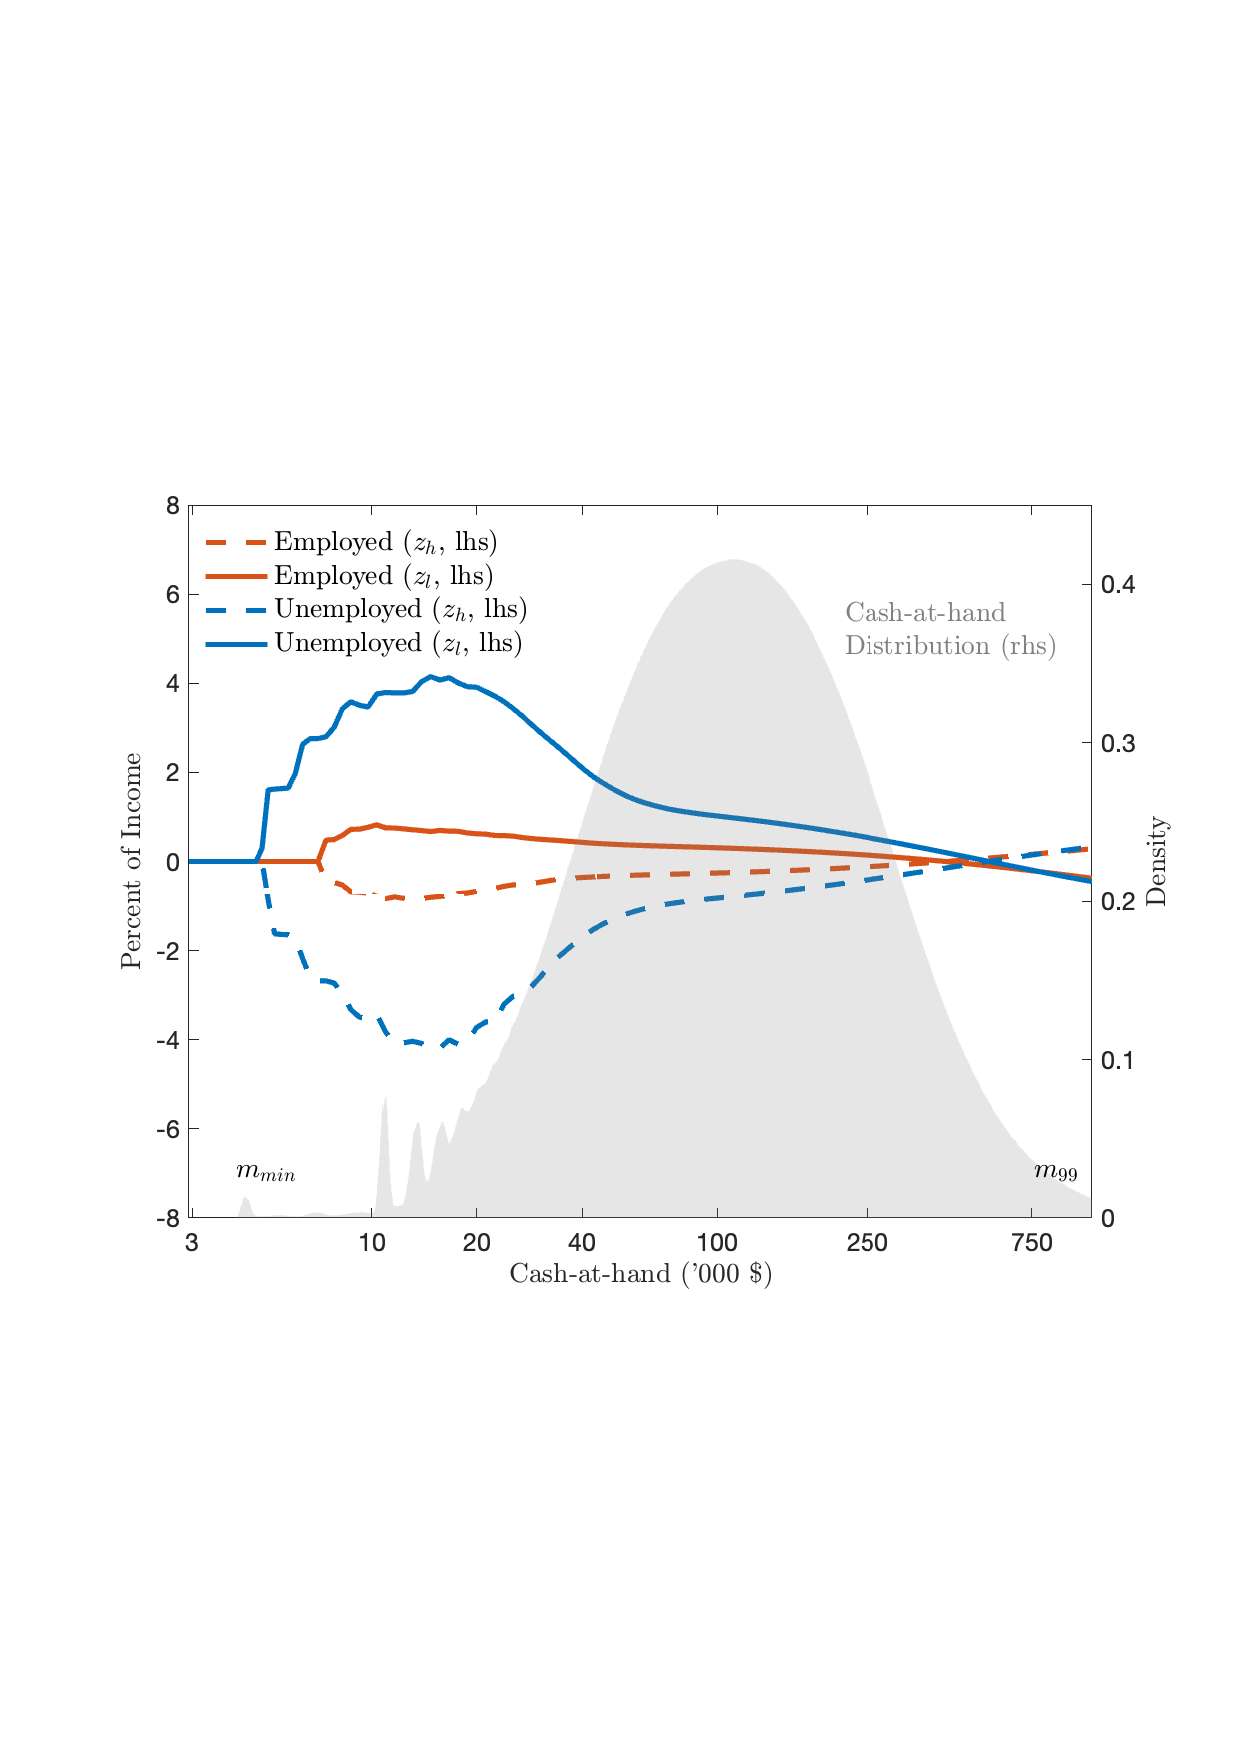
\includegraphics[width=\linewidth,trim=29 160 29 224,clip]{_input/figure_4a.pdf}
% \includegraphics[width=\linewidth,trim=29 160 29 224,clip]{_input/savingsinformeduninformed.pdf}
\end{subfigure}\hfill
\begin{subfigure}[t]{0.48\textwidth}
  \centering
  \caption{Informed $\pm \sigma(K_t)$ vs. Uninformed}
  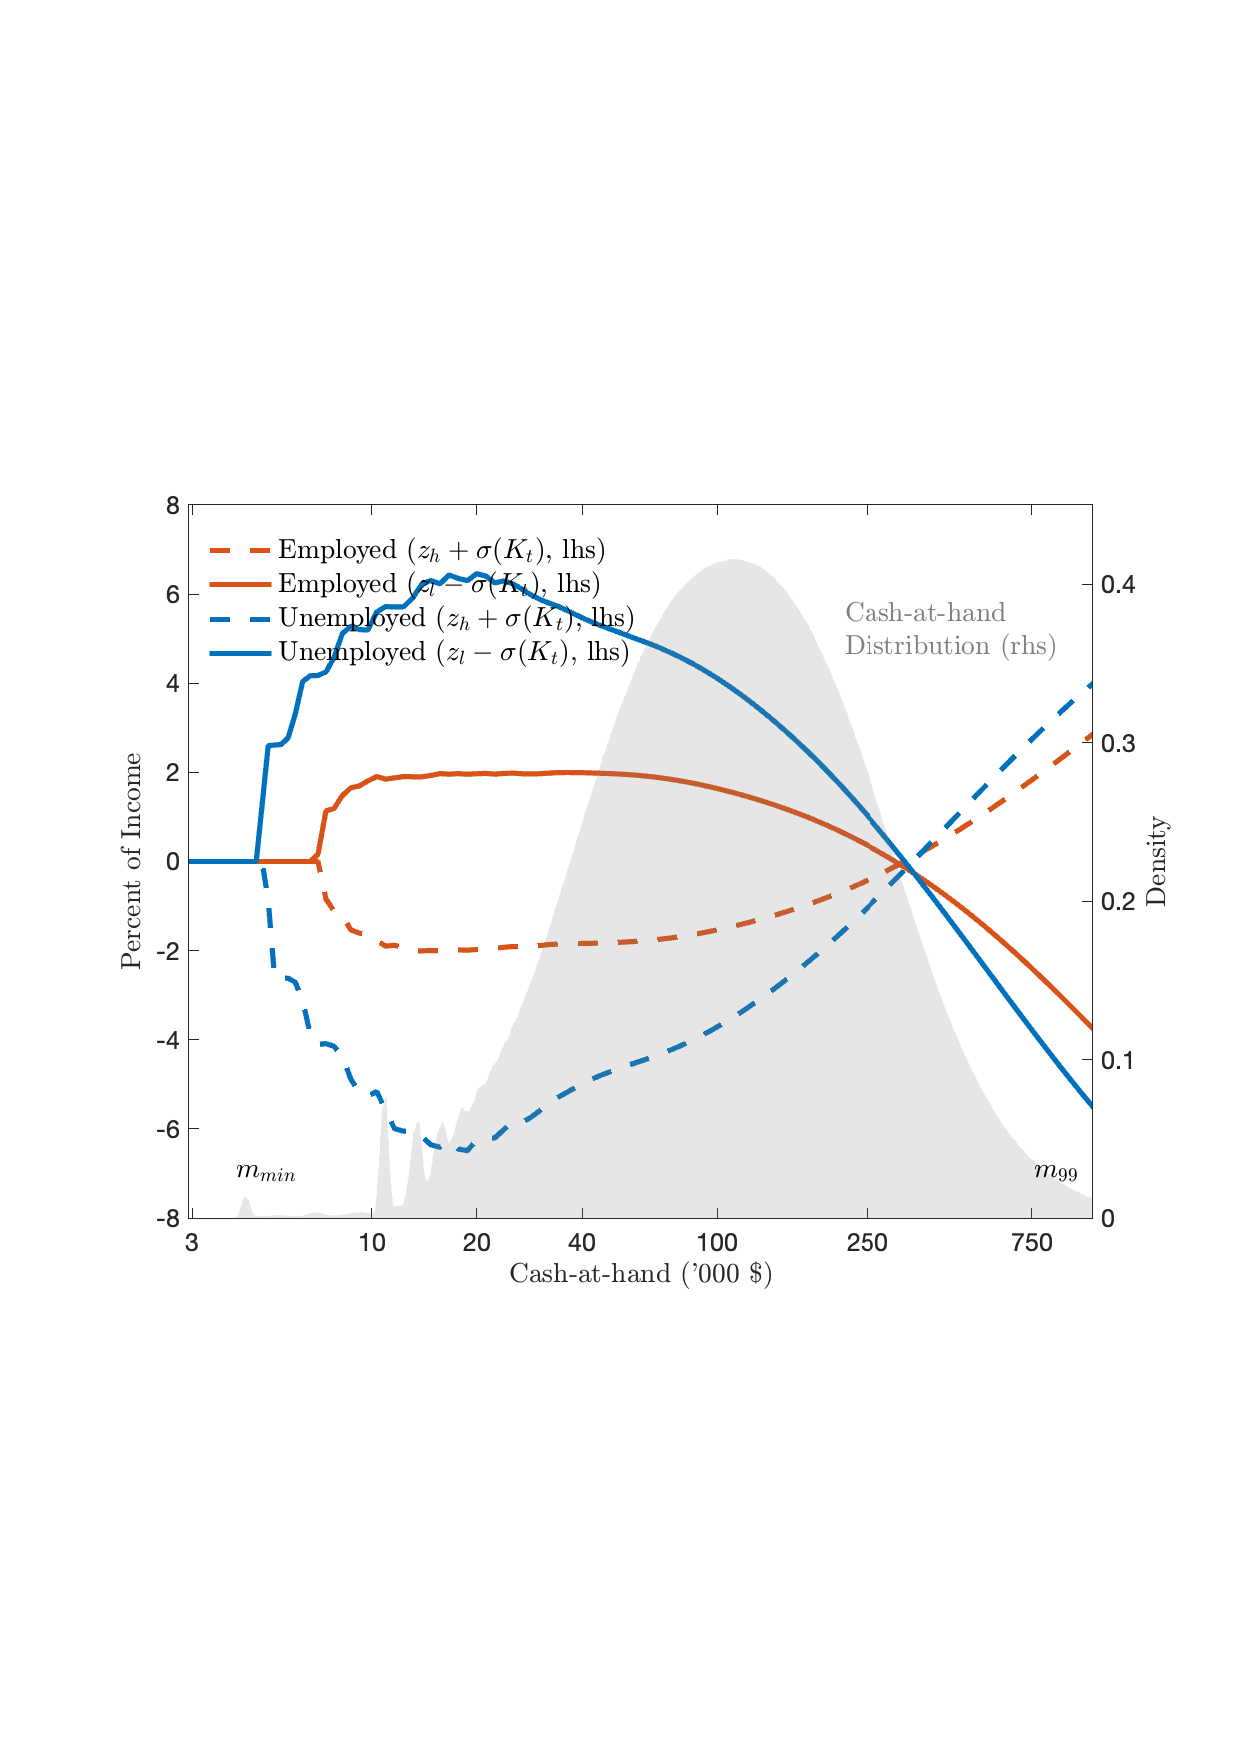
\includegraphics[width=\linewidth,trim=29 160 29 224,clip]{_input/figure_4b.pdf}
% \includegraphics[width=\linewidth,trim=29 160 29 224,clip]{_input/savingsinformeduninformedcapital.pdf}
\end{subfigure}

\vspace{-0.47cm}
\footnotesize

%\justifying
\noindent                {\protect\footnotesize \textit{Note:}  The figure  plots the difference between the savings choice of ``an informed household'', who has just acquired information about $z$,  and ``an uninformed household''
in our benchmark economy as a percent of household income. An uninformed household has a 50-50 prior over productivity $z$. We plot this difference in a recession (solid lines, $z=z_l$) and a boom (dashed lines, $z=z_h$) for both an unemployed (in blue) and employed (in red) household, and overlay the distribution of cash-at-hand in the benchmark economy in gray. Panel (a) plots the difference evaluated  at the mean prior for capital,  while Panel (b) instead evaluates the savings choice of the informed household at a prior over the capital stock that is 1 standard deviation higher (lower) than the mean in a boom (bust). We plot savings differences as a function of cash-at-hand and use  2020 values of U.S. household income to convert values into USD (\$) amounts.
}
\end{figure}

\vspace{0.29cm}

\noindent\textbf{Comparison of Informed to Uninformed. }Instead,
what drives the often substantial differences \emph{is the different
savings behavior of uninformed households}. We contrast these to informed
households' savings choices in Figure \ref{fig:4-savings-choices},
where we plot savings differences (``informed minus uninformed'')
in the benchmark economy as a function of a household's cash-at-hand.
Panel (a) assumes both households share the same expectation of the
capital stock, while Panel (b) internalizes that an informed household's
expectation of capital will also be different. Combined, the two panels
show large differences in savings\textemdash up to around 6\% of income\textemdash across
much of the cash-at-hand distribution, especially for unemployed households
and after one accounts for how information also alters household expectations
of capital. The presence of incomplete information matters for the
bulk of households.

Crucially, Figure \ref{fig:4-savings-choices} documents substantial
variation in savings differences across the cash-at-hand distribution.
\emph{Below around the 85th percentile, uninformed households save
more procyclicall}y\emph{ than informed ones}.\textcolor{orange}{{}
}While informed households save more in recessions ($z_{l}$) and
less in booms ($z_{h}$), uninformed households do the opposite; they
save comparatively less in recessions and more in booms. However,
unlike this majority of households, above the 90th percentile the
pattern instead reverses: \emph{Uninformed rich households save more
in recessions and less in booms; their savings are}\textcolor{orange}{{}
}\emph{are instead more} \emph{countercyclical.} Taken together, this
shows how the wealth distribution can shape the overall cyclicality
of savings. We return in Section \ref{subsec:aggregate-implications}
to how the net-effect of these countervailing forces amplifies business
cycles.\vspace{0.29cm}

\noindent\emph{Information about Productivity:}\textbf{ }To understand
this varying cyclicality, start with Panel (a) in Figure \ref{fig:4-savings-choices}
that shows the savings differences caused by information about productivity
alone. The poorest households optimally reduce capital holdings to
zero independent of the state of the economy. As such, information
does not change their savings behavior. Savings rates of informed
households, by contrast, differ strongly from those of the uninformed
households at low-but-positive levels of cash-at-hand, where the non-linearity
of the savings policy function is pronounced near the kink at the
borrowing constraint. Information about productivity helps such households
better predict the probability of employment and future wages, and
thus future labor income, which is the main determinant of future
consumption for low-wealth households. Informed households, as a consequence,
save more in recessions and less in booms. This difference between
informed and uninformed savings is especially pronounced for unemployed
households, whose job-finding rate differs strongly across booms and
busts. 

As cash-at-hand increases, the difference between informed and uninformed
savings initially declines. In this region, errors about future labor-market
prospects and capital returns push savings in opposite directions.
Optimistic expectations about the job-finding rate in a bust, for
example, reduces precautionary savings, while expecting a higher return
on capital raises savings through intertemporal substitution.\textcolor{orange}{{}
}As one moves towards the middle of the wealth distribution, these
effects partially offset each other, lowering savings differences
between informed and uninformed households.\footnote{The moderate persistence of productivity shocks entails only ever
weak income effects. This decline is further reinforced by the savings
function becoming increasingly linear.} At even higher wealth levels\textemdash above around the 90th percentile\textemdash the
savings differences eventually flip sign, as financial assets comprise
the bulk of household resources. Variations in returns here dominate
household savings choices, leading to increasing savings differences,
as intertemporal substitution makes informed households save more
in booms and less in recessions. \vspace{0.29cm}

\noindent\emph{Information about Capital:}\textbf{ }While knowing
the current productivity state is important, acquiring information
also causes households to perceive the economy's endogenous dynamics
more accurately\textemdash particularly the evolution of the capital
stock. Recall that in Panel (a) of Figure \ref{fig:4-savings-choices}
informed and uninformed households have the same expectation of capital.
Any perceived differences in wages and rates of return from being
informed stem only from perceived differences in productivity and
hence employment prospects. With incomplete information, however,
uninformed households also perceive less accurately the dynamics of
capital (that rises in booms and falls in recessions). Their expectations
about future capital, returns and wages, are less cyclical and biased
towards the unconditional mean. We illustrate how such mean-biased
capital expectations change savings behavior in Panel (b) of Figure
\ref{fig:4-savings-choices}.

Compared to Panel (a), having mean-biased capital expectations increases
the magnitude of savings mistakes that the vast majority of households
make. The additional effect is especially pronounced for low-wealth
households and households above the 90th percentile, whose savings
mistakes are amplified by a factor between 1.5 and 4.0. These savings
mistakes are explained by errors in households' expectations of future
wages and returns, crucial for low- and high-wealth households' savings
choices, respectively. Both now combine errors due to (i) mistaken
\emph{exogenous components} of labor income and returns (i.e., productivity
and employment transitions); and (ii) a mistaken \emph{endogenous
component} (i.e., capital accumulation). Since a higher capital stock
in booms, for example, provides an additional, persistent boost to
future labor income through higher wages, informed savings by the
poor are reduced by more relative to the savings of the uninformed\textemdash both
components compound each other. Similarly, income effects from reduced
returns at a higher aggregate capital stock boost savings of the informed
rich further relative to those of the uninformed.\footnote{Note the compounding effects of information about productivity and
the capital stock on rich households' informed savings: Higher returns
during moderately persistent productivity booms have weak income effects,
and thus increase savings through a substitution effect (Panel a of
Figure \ref{fig:4-savings-choices}). Diminishing returns from highly
persistent increases in the capital stock have strong income effects,
further boosting savings as capital accumulates (Panel b of Figure
\ref{fig:4-savings-choices}).}

\medskip

Combined, Figures \ref{fig:3-savings-choices} and \ref{fig:4-savings-choices}
show that an absence of information about exogenous and endogenous
components substantially alters household savings, with the direction
and magnitude of distortions varying across the wealth distribution.
These individual-level distortions have the potential to significantly
affect macroeconomic outcomes, depending on which households are uninformed
in equilibrium. We next explore how the above forces interact to shape
households' information choices. This will cast further light on the
wealth-expectations nexus.

\subsection{Household Information Choices\label{subsec:information-choice}}

Information choices are most easily described by the probability of
acquiring information. Figure \ref{fig-3-information-prob} plots
this probability as a function of a household's state variables\textemdash cash-at-hand
and the prior over productivity\textemdash separately for the employed
and unemployed, and for a low and a high prior over the capital stock.
Combined, the results in Figure \ref{fig-3-information-prob} showcase
the rich heterogeneity that exists in incentives to acquire information.
Unsurprisingly, households with less informative prior expectations
(closer to one half) are more likely to acquire information for all
wealth levels, except those at the borrowing constraint.

\begin{figure}
\caption{Information Acquisition Probabilities}
\label{fig-3-information-prob}\vspace{0.38cm}
\begin{centering}
\hspace{0.90cm}Panel (a): Unemployed, Low Prior $K_{t}$\hspace{2.30cm}Panel
(b): Employed, Low Prior $K_{t}$\\\hspace{-0.92cm}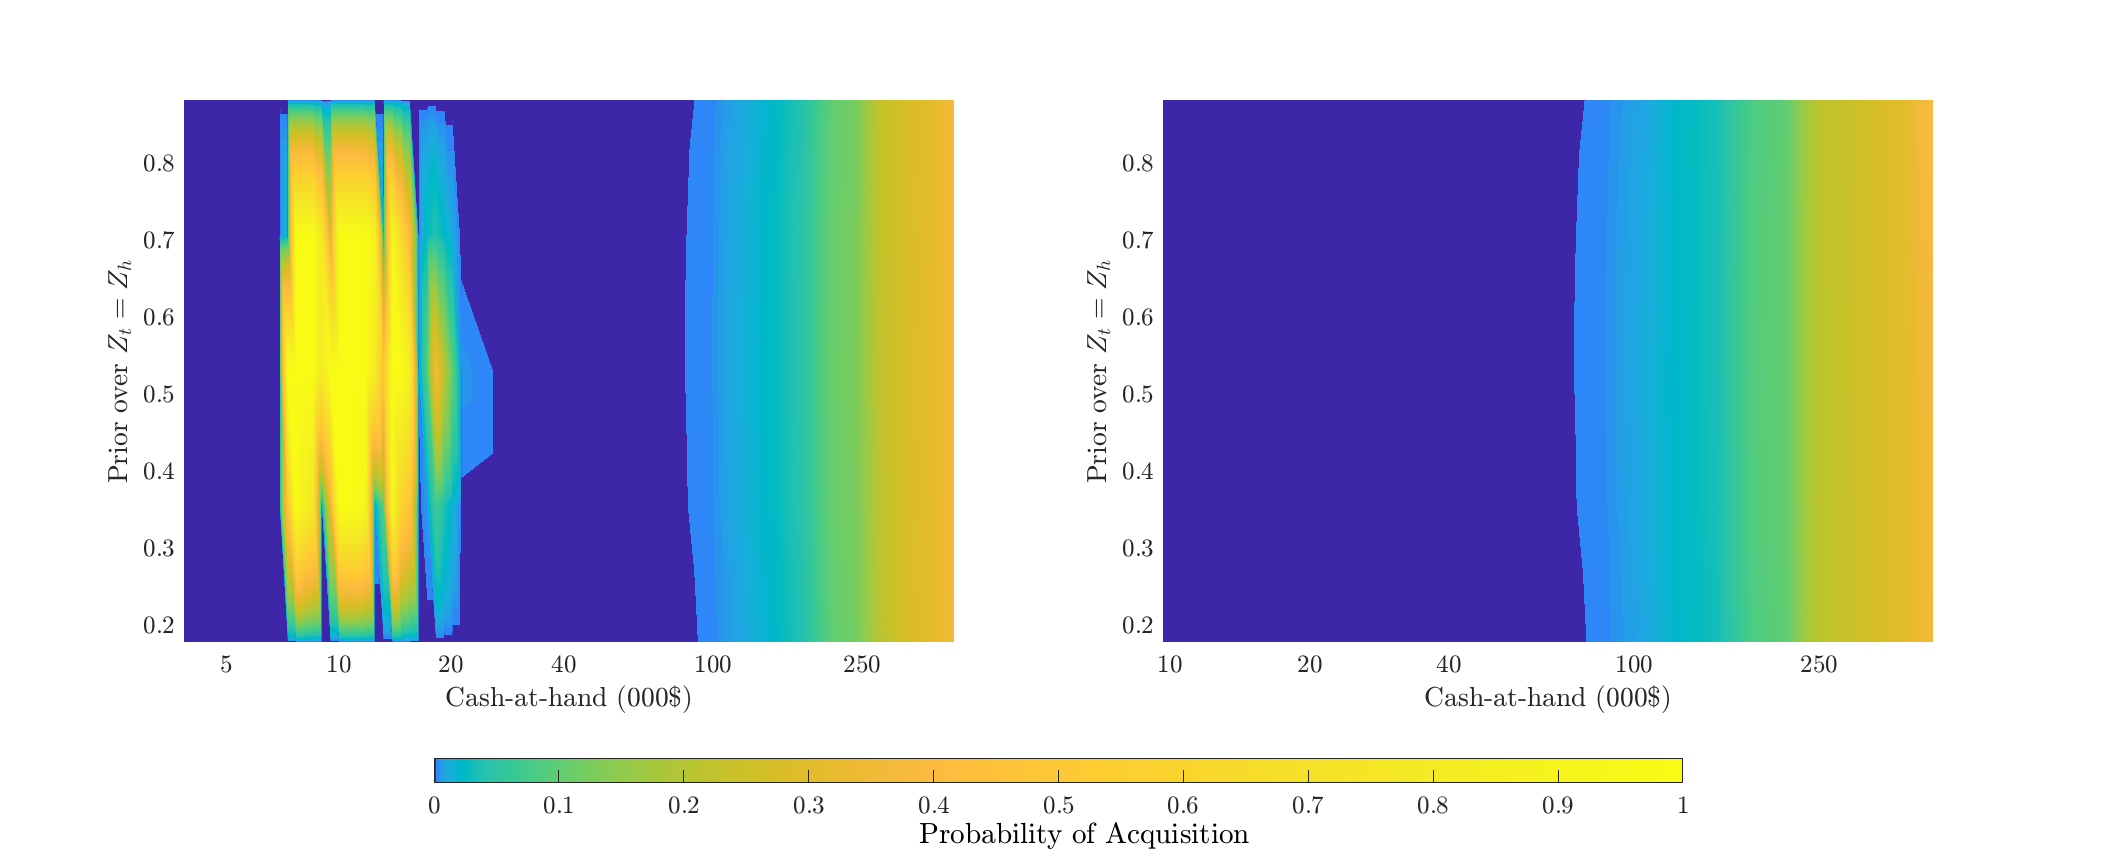
\includegraphics[viewport=43bp 0bp 1000bp 360bp,clip,scale=0.54]{_input/figure_5ab}\vspace{0.38cm}
\par\end{centering}
\begin{centering}
\hspace{0.90cm}Panel (c): Unemployed, High Prior $K_{t}$\hspace{2.05cm}Panel
(d): Employed, High Prior $K_{t}$\\\hspace{-0.92cm}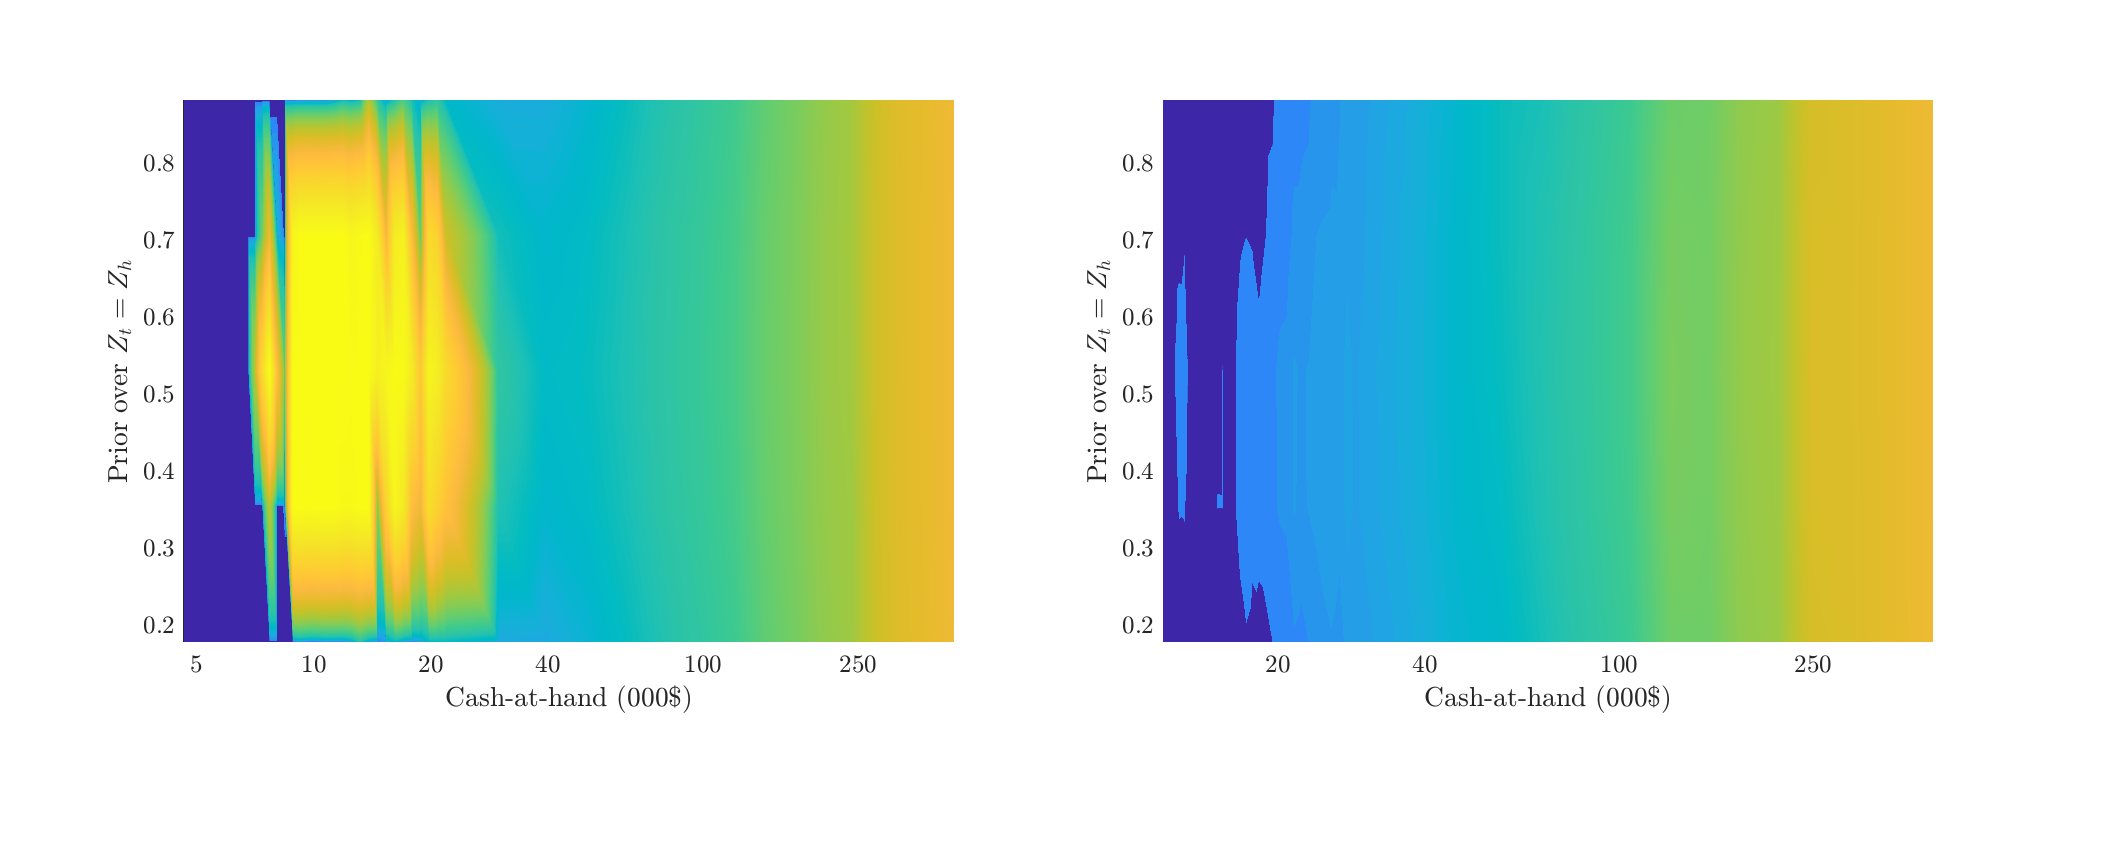
\includegraphics[viewport=43bp 35bp 1000bp 360bp,clip,scale=0.54]{_input/figure_5cd}
\par\end{centering}
{\footnotesize\emph{Note}}{\footnotesize : The figure plots the probability
of information acquisition (from 0 to 1) for different values of the
prior belief that current productivity $z_{t}$ is high and for different
values of household cash-at-hand. The figure uses our baseline calibration
to depict the probabilities and evaluates them at a ``low'' (i.e.,
25\% below the mean) and ``high'' (i.e. 25\% above the mean) prior
over the aggregate capital stock $K_{t}$. The left-hand (right-hand)
panels show the probabilities for an unemployment (employed) household.
We use 2020 values of U.S. household income to convert cash-at-hand
in our model to USD (\$) amounts.}{\footnotesize\par}
\end{figure}

\emph{Employed} \emph{households}\textemdash the savers in the economy\textemdash are
less likely to acquire information, especially at low levels of wealth.
Because separation rates are only mildly cyclical (5.0 percent in
recessions and 3.5 percent in booms), their optimal savings change
comparatively little across boom-bust states (Figure \ref{fig:4-savings-choices}).
With low unemployment risk and a moderate persistence of boom-busts,
they are further unlikely to hit the borrowing constraint soon. Thus,
they expect to continue to accumulate assets over time, so that the
average savings error from remaining uninformed is relatively small,
as discussed in the previous section. The option to acquire information
after a future job loss further lowers the value of doing so today.
As wealth rises, however, the benefit of predicting returns on increasing
financial wealth rises and the cost of acquiring information relative
to wealth falls, increasing the probability of information acquisition.
Indeed, households with more than \$300,000 in cash-at-hand acquire
information close to 50 percent of the time (Panel (b) and (d) in
Figure \ref{fig-3-information-prob}). This compares to an overall
average rate of information acquisition of 10 percent. 

Now, consider instead \emph{unemployed households}. The unemployed
are dissavers, as they attempt to smooth consumption. At low enough
values of cash-at-hand, they consume their resources and end up at
the borrowing constraint. Thus, at sufficiently low values, unemployed
households almost never acquire information. These households are
at the borrowing constraint for all states that realize tomorrow,
and hence have no benefit from acquiring information today (Figure
\ref{fig:4-savings-choices}). However, at slightly higher values
of cash-at-hand, unemployed households start to acquire information
with high probability\textemdash to avoid large savings mistakes from
not knowing the state of the economy (Figure \ref{fig:4-savings-choices}).
Savings mistakes from being uninformed are costly near the borrowing
constraint where\textcolor{orange}{{} }the curvature of both the utility
function and policy functions is high. In this range of the wealth
distribution, unemployed households thus almost uniformly  acquire
information (Panel (a) and (c) in Figure \ref{fig-3-information-prob}).\footnote{The same incentives raise information-acquisition probabilities of
uninformed employed households, who face a smaller but positive probability
of becoming unemployed, at moderate levels of cash-at-hand, as seen
in Panel (d) in Figure \ref{fig-3-information-prob}.} 

As wealth rises further, marginal utility eventually falls, and the
value of information initially declines. The household is no longer
at risk of imminently hitting the constraint, and expectation errors
about the labor market and capital returns have opposing effects on
savings, lowering savings differences due to information (Figure \ref{fig:4-savings-choices}).
This temporarily lowers the value of information. The value of information,
nevertheless, then slowly starts to rise again with wealth for the
same reasons as discussed for the case of the employed.

Finally, notice that households with low-levels of wealth are, on
balance, more likely to acquire information when their prior about
the current capital stock is high (Panel (c) and (d) in Figure \ref{fig-3-information-prob}).
This is because higher wages implied by abundant capital increase
the dispersion of incomes across employment states. This increases
the value of accurately predicting employment prospects, and thus
the probability of information acquisition.

\subsection{Accuracy of Expectations\label{subsec:results-accuracy}}

We have described how wealth and employment status affect a household\textquoteright s
decision to acquire information, and how a household\textquoteright s
savings decision is in turn affected by the accuracy of its information.
Before we turn to the macroeconomic consequences of the two-sided
interaction between household heterogeneity and information choice,
we study how these forces interact to shape the accuracy of household
expectations across the wealth distribution. This will also allow
us to confront our model with the empirical evidence discussed in
Section \ref{sec:motivating-evidence}.

\begin{figure}[t]
\caption{Accuracy of Forecasts: Model vs. Data}
\label{fig-5-accuracy-u}\vspace{0.22cm}
\begin{centering}
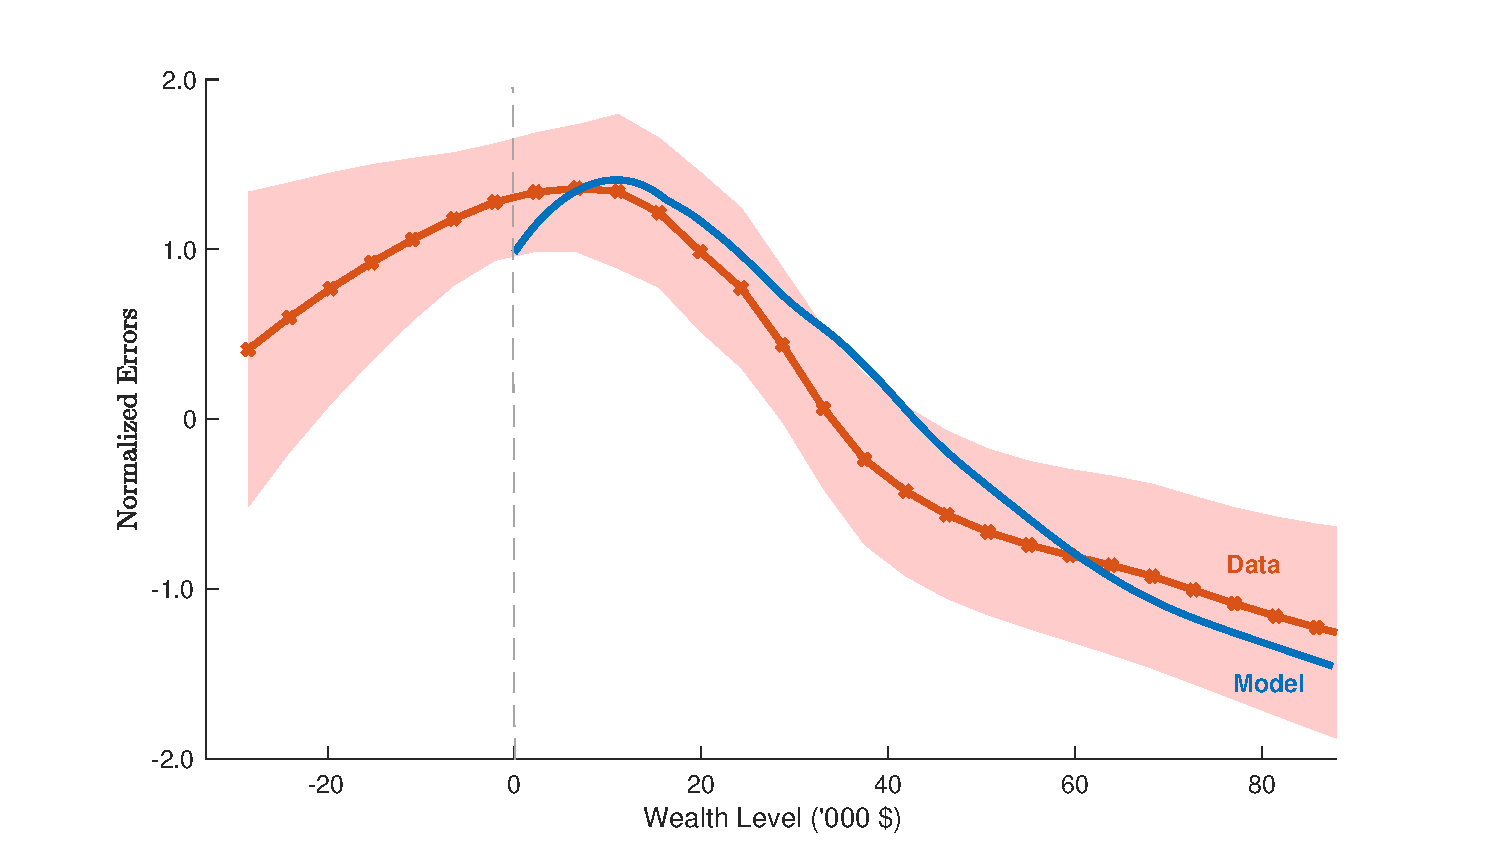
\includegraphics[viewport=25bp 0bp 1000bp 400bp,clip,scale=0.74]{_input/figure_6}
\par\end{centering}
{\footnotesize\emph{Note}}{\footnotesize : The figure shows the estimated
relationship between (the absolute value of) normalized errors of
the one-year ahead probability of the unemployment rate increasing
and household wealth. We plot this relationship both in the SCE data
and in the calibrated model (see also Section \ref{sec:motivating-evidence}).
We use a local polynomial regression (the LOESS regression) to estimate
the non-linear relationship between the accuracy of household expectations
and household wealth. Error bands correspond to one-standard deviation
confidence bounds. We use 2020 values of quarterly U.S. household
income to convert values in the data and in the model to \$ (USD)
amounts.}{\footnotesize\par}
\end{figure}

Figure \ref{fig-5-accuracy-u} shows how households\textquoteright{}
information acquisition probabilities in equilibrium translate into
a systematic relationship between the accuracy of household expectations
and their wealth level. Because the model matches the mean and standard
deviation of absolute errors, Figure \ref{fig-5-accuracy-u} plots
normalized errors in both the model and in the data (Figure \ref{fig-5-accuracy-u-2}
shows errors relative to the top quintile and extends the horizontal
axis). For compatibility with the SCE data, we plot errors as a function
of household wealth $k_{i}$ instead of cash-at-hand $m_{i}$. Although
our model cannot speak to the positive slope that exists in the data
for households with negative wealth\textemdash recall that we assume
a simple no-borrowing limit $k_{i}^{\prime}\geq0$ for households\textemdash the
model generates an inverse-u shape, which on balance resembles that
in the survey data.

The inverse-u shape in the model is a result of two opposing forces:
First, the upward sloping part  is driven by the unemployed. The poorer
households in the model are, on average, the unemployed, who at low
levels of wealth acquire information with high probability. As those
households find jobs, their wealth increases but they also stop acquiring
information, leading to the observable decline in  accuracy at low
levels of wealth. Second, as wealth increases, the probability of
acquiring information eventually becomes monotonic in wealth (Figure
\ref{fig-3-information-prob}). As wealth rises, the benefits of information
about its return increases and the relative cost falls\textemdash both
of which increase a household's information acquisition probability
and thus accuracy. We conclude that the model, on balance, successfully
replicates the salient features of the empirical wealth-expectations
relationship, making it a suitable laboratory to explore the effects
of expectation heterogeneity on the macroeconomy.

\subsection{Aggregate Implications\label{subsec:aggregate-implications}}

Our analysis so far has centered on the savings and information choices
of an individual household. In this subsection, we document how the
heterogeneity in savings and information choices depicted in Figures
\ref{fig:4-savings-choices} and \ref{fig-3-information-prob} accumulate
to amplify business-cycle fluctuations.

In Table \ref{tab:business-cycle-moments}, we contrast the dynamics
of our benchmark economy with those that arise in the full-information
economy, where all households exogenously acquire information every
period. Recall that, on average, only around 10 percent of households
choose to acquire information in any given period under our baseline
calibration. We also compare the dynamics from our model with those
that arise from an economy in which all households face the same (exogenous)
10 percent probability of information acquisition in every period
à la \citet{mankiw2002sticky}. In a slight abuse of terminology,
we refer to this economy as the ``exogenous-information economy''.\footnote{Notice that the full-information economy is merely an exogenous-information
economy with the probability of information acquisition fixed at 1.
We keep the ``full-information'{}'' and ``exogenous-information''
labels in what follows to clarify that any comparison between the
two focuses on the \emph{incompleteness} of information. A comparison
between our benchmark economy and the exogenous-information economy,
by contrast, focuses on the consequences of \emph{heterogeneity} in
information.}\textcolor{orange}{{} }In both cases, we assume households pay the resource
and utility cost of information upon acquisition, and recalibrate
the discount factor to target the same capital-to-output ratio.\textcolor{orange}{{}
}Section \ref{sub-sect-ext:cost} compares our results to the case
where households do not pay these costs. Table \ref{app-tab:bc-moments}
further compares the business-cycle dynamics to those in the U.S.\footnote{Compared to the data (Table \ref{app-tab:bc-moments}), our model
features the same deficiencies synonymous with workhorse RBC or \citet{KS98}
economies: Investment is too volatile, consumption too smooth, and
output is, as a result of employment and investment dynamics, too
volatile. We abstract from these deficiencies in what follows below,
as our focus is squarely on the consequences of the wealth-expectation
nexus.}

\begin{table}[t]
\caption{Business Cycle Moments}

\label{tab:business-cycle-moments}\textcolor{black}{\vspace{-0.29cm}}

\textcolor{black}{\def\sym#1{\ifmmode^{#1}\else\(^{#1}\)\fi}

%\begin{tabular*}{\textwidth}{@{\extracolsep{\fill} } l c c c c c c}
\begin{tabular*}{\textwidth}{l C{1.97cm} C{1.97cm} C{1.97cm} C{1.97cm} C{1.97cm} C{1.97cm}}
\toprule \toprule\\[-1.8ex]
& \multicolumn{5}{c}{Panel (a): Level of Moments}\\
& $\sigma(K)$ & $\sigma(Y)$ & $\sigma(I)$ & $\sigma(C)$ &$\text{Cor}(C,Y)$ \\
\cline{2-6} \\[-1.8ex]
Benchmark  Model                  & 5.05 & 3.38 & 11.98 & 1.25 & 0.70 \\
[1em] Exogenous Information  & 4.19 & 3.22 & 11.56 & 1.19 & 0.67  \\
[1em] Full Information              & 3.07 & 3.04 & 10.54 & 1.19 & 0.72  \\
\hline
&&&\\
& \multicolumn{5}{c}{Panel (b): Percent  Difference w.r.t. Full Information} \\ 
& $\sigma(K)$ & $\sigma(Y)$ & $\sigma(I)$ & $\sigma(C)$ & $\text{Cor}(C,Y)$  \\
\cline{2-6}\\[-1.8ex]
Benchmark Model                    & 64.28 & 11.04 & 13.63 & 5.11 & -3.07\\ 
[1em]  Exogenous Information & 36.46 & 5.84 & 9.65 & 0.31 & -7.24\\ 
\bottomrule
\bottomrule
\end{tabular*}
}

\vspace{0.22cm}

{\footnotesize\emph{Note}}{\footnotesize : The table shows the standard
deviation $\sigma\left(\cdot\right)$ of the logarithms of economy-wide
capital ($K$), output ($Y)$, investment ($I$), and consumption
($C)$. In addition, the table shows the correlation between log.
consumption and output, $Cor(C,Y)$. The table computes these moments
in the calibrated economy (``Benchmark Model''), the associated
full-information economy (``Full Information''), as well as in a
model with an exogenously specified probability of acquiring information
(``Exogenous Information''). The probabilities of information acquisition
in the benchmark model are 0.122 and 0.097, respectively, for the
unemployed and employed. This probability is set equal to 0.10 in
the exogenous information case.}{\footnotesize\par}
\end{table}
Relative to the full-information case, fluctuations in all aggregate
variables are substantially more pronounced in our benchmark economy.
The standard deviation of capital is around 2/3 higher, and output
and consumption are, as a result, 5-11 percent more volatile than
in the full-information economy. These stark differences are caused
by the increased procyclicalty and persistence of capital, driven
by heterogeneous incomplete information.

As discussed in Section \ref{subsec:savings-information-nexus}, the
central difference between the savings choices in the benchmark economy
and its full-information counterpart is the different savings behavior
of \emph{uninformed households}. Households who choose \emph{not}
to acquire information\textemdash who comprise 90 percent of the population\textemdash have
expectations that are tilted towards the long-run average of the economy.
In booms, such households systematically underpredict productivity
and the capital stock, and hence future labor income, and vice versa
in recessions.\footnote{We should note, however, that a hypothetical household that acquires
information in every period would have an accurate estimate of the
true capital stock and make negligible forecast errors (Appendix \ref{app:model-fit}).} Consequently, households below the 85th percentile save more in booms
and less in recessions than if they had full information\textemdash their
savings are more procyclical (Figure \ref{fig:4-savings-choices}).
Wealthy households above 90th percentile, by contrast, make the opposite
mistake, but because these households acquire information more frequently
and control less of the capital stock (Figure \ref{fig:4-savings-choices}
and \ref{fig-3-information-prob}), they do not not offset the procyclical
forces from the majority. In equilibrium, the economy thus systematically
``overaccumulates'' capital in booms and ``underaccumulates''
in recessions, leading to much larger fluctuations in output and investment
than under full-information.

Figure \ref{fig:IRFs} illustrates the weakened mean-reversion and
amplification; it does so by plotting the economy\textquoteright s
response to a negative productivity shock (a transition from $z_{h}$
to $z_{l}$). Consistent with Table \ref{tab:business-cycle-moments},
the impulse responses are substantially larger and more persistent
in the benchmark economy. Panel (b) shows that capital decreases in
all cases and that even after several years the shock has yet to die
out; however, importantly, the speed of recovery is substantially
slower in our benchmark economy, due to the increased procyclicality
of savings. There is \emph{substantially more} \emph{internal propagation}.
Panel (d) shows the investment response behind this difference. Panel
(c) mirrors these results and shows that output, as a consequence,
falls by similar amounts on impact but that the recovery is substantially
more protracted in the benchmark economy. Because of heterogeneous
incomplete information, business cycles are amplified and more protracted\textemdash and
the IRFs directly illustrate the mechanism.

Compared to the exogenous-information case, where all households have
the same probability of acquiring information, the endogeneity of
information that is a feature of our benchmark economy further amplifies
the increase in aggregate volatility (Table \ref{tab:business-cycle-moments};
Figure \ref{fig:IRFs}). This occurs because middle-wealth households
who combine to hold most of the capital stock acquire information
with less than average frequency (Figure \textcolor{orange}{\ref{fig-3-information-prob}}).
This further dampens the mean-reversion of capital in our benchmark
economy relative to an economy in which all households have the \emph{same
probability} of acquiring information. The \emph{heterogeneity}\emph{
in information choices} amplifies the consequences of incomplete information.

\begin{figure}[t!]
    \begin{center}
		%\centering
		\caption{Impulse Response Functions}
    \label{fig:IRFs}
    \begin{subfigure}{0.49\textwidth}
        \centering
        \caption{Productivity}
        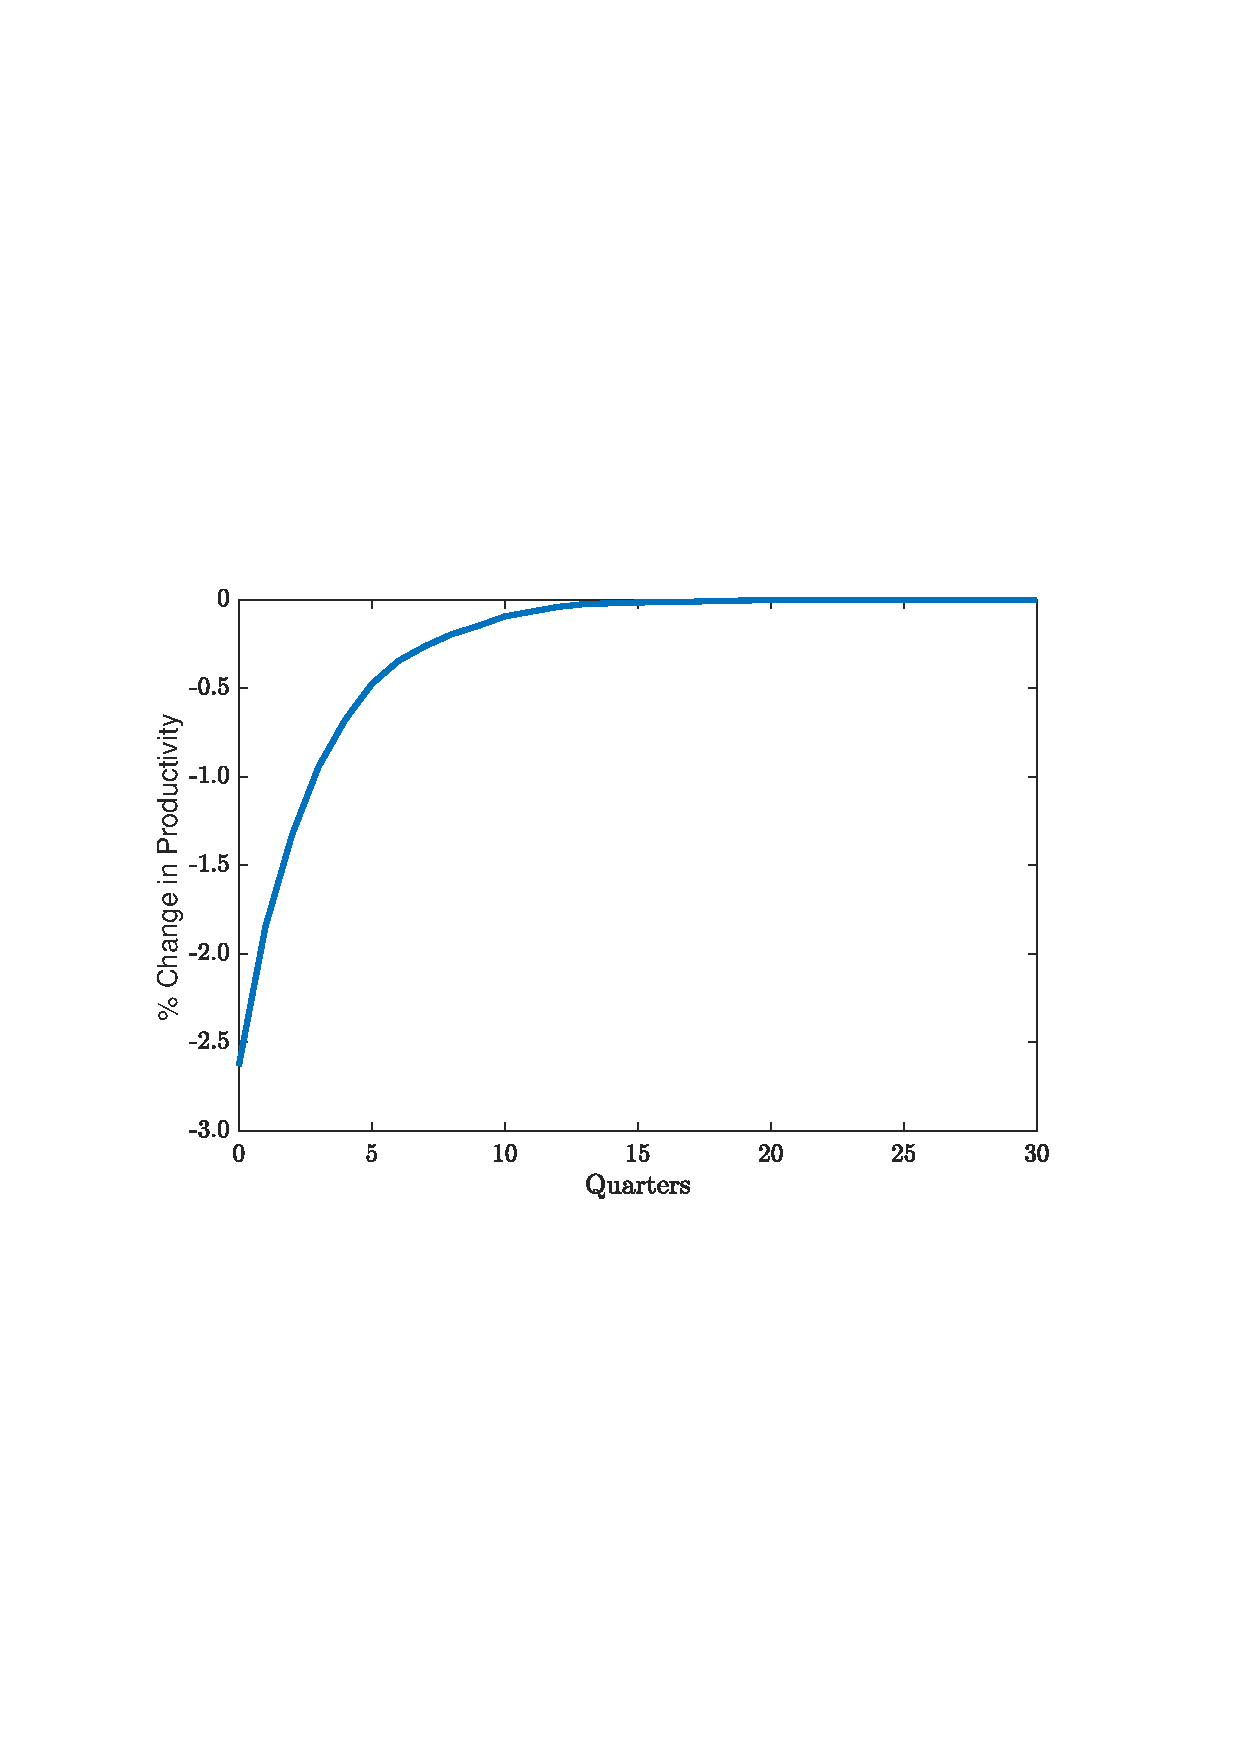
\includegraphics[width=\linewidth,trim=60 250 60 280,clip]{_input/figure_IRF_prod2.pdf}
        %\label{fig:a}
    \end{subfigure}
    \hfill
    \begin{subfigure}{0.49\textwidth}
        \centering
        \caption{Capital}
        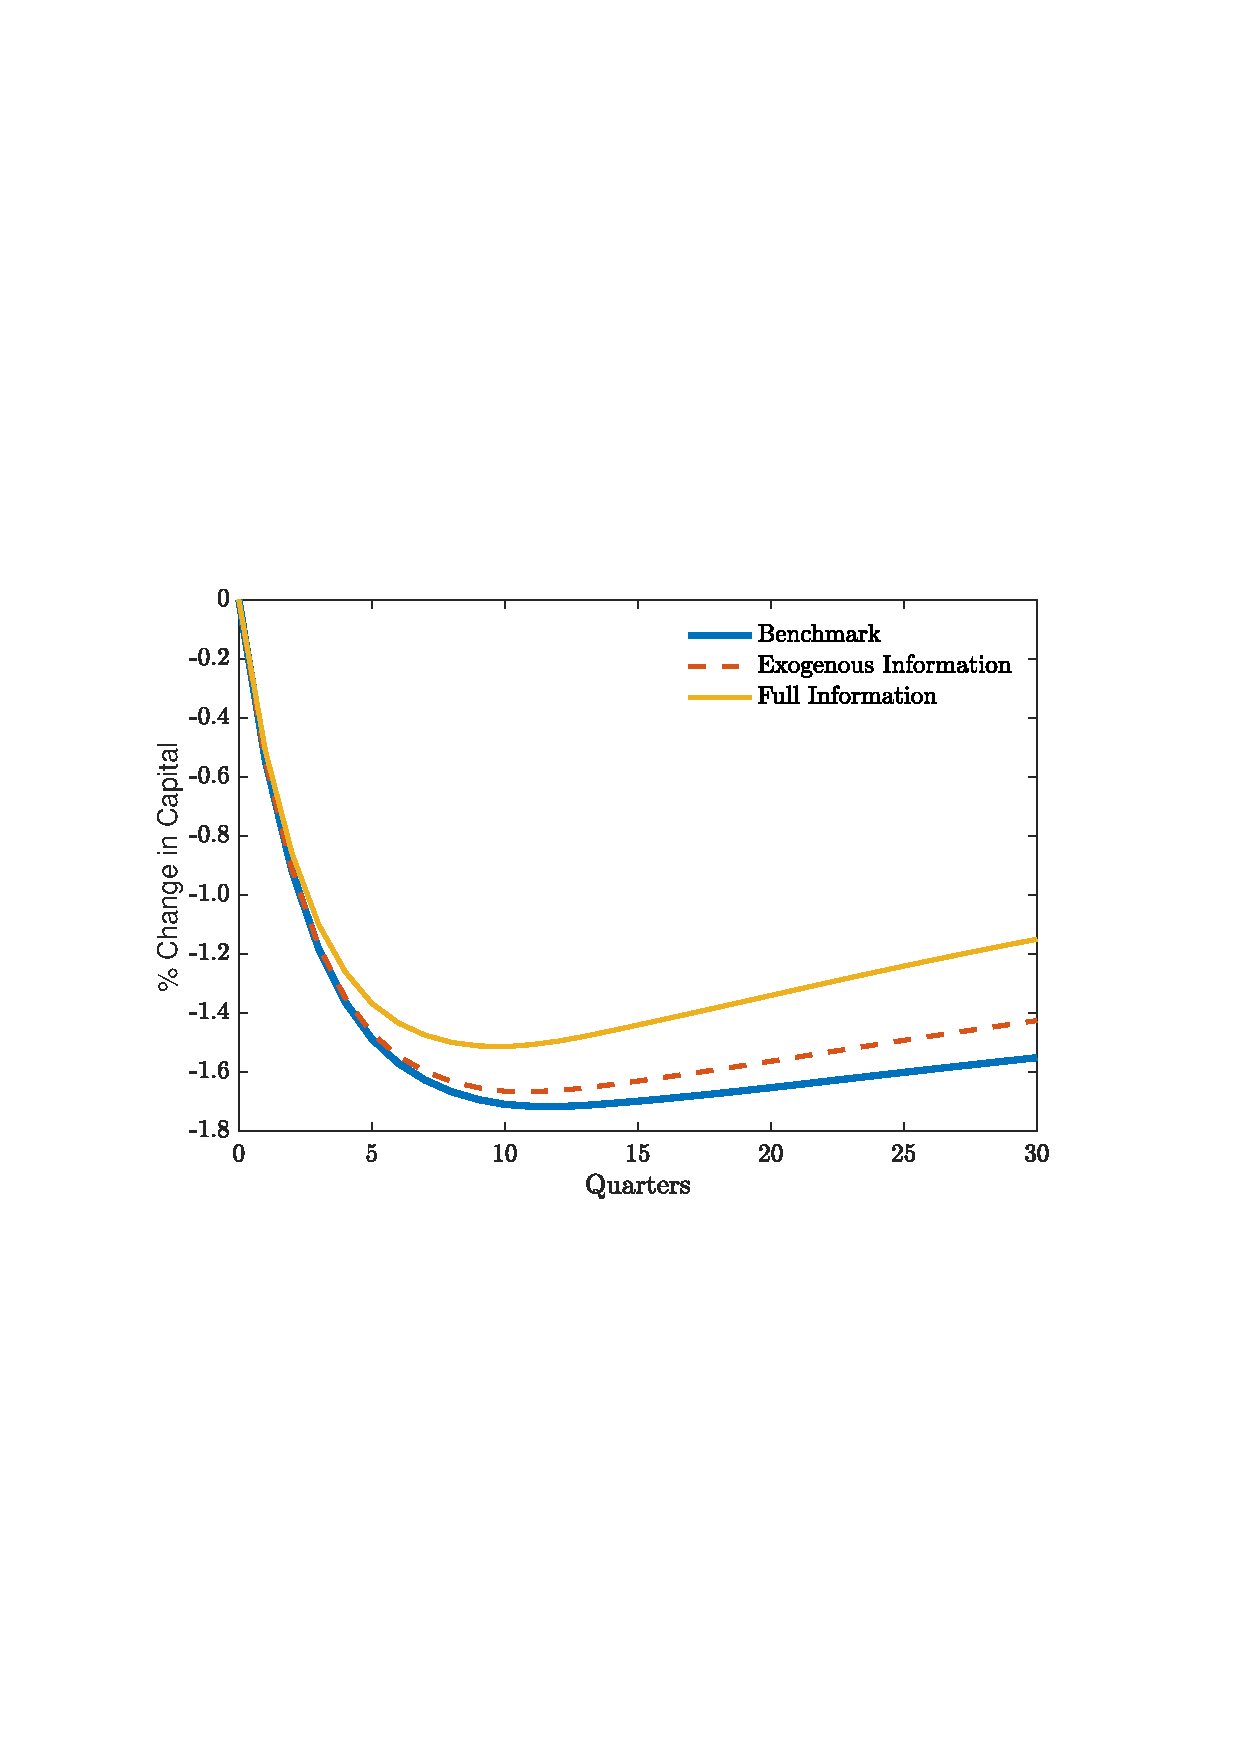
\includegraphics[width=\linewidth,trim=60 250 60 280,clip]{_input/figure_IRF_k2.pdf}
        %\label{fig:c}
    \end{subfigure}
		\hfill
    \begin{subfigure}{0.49\textwidth}
        \centering
        \caption{Output}
        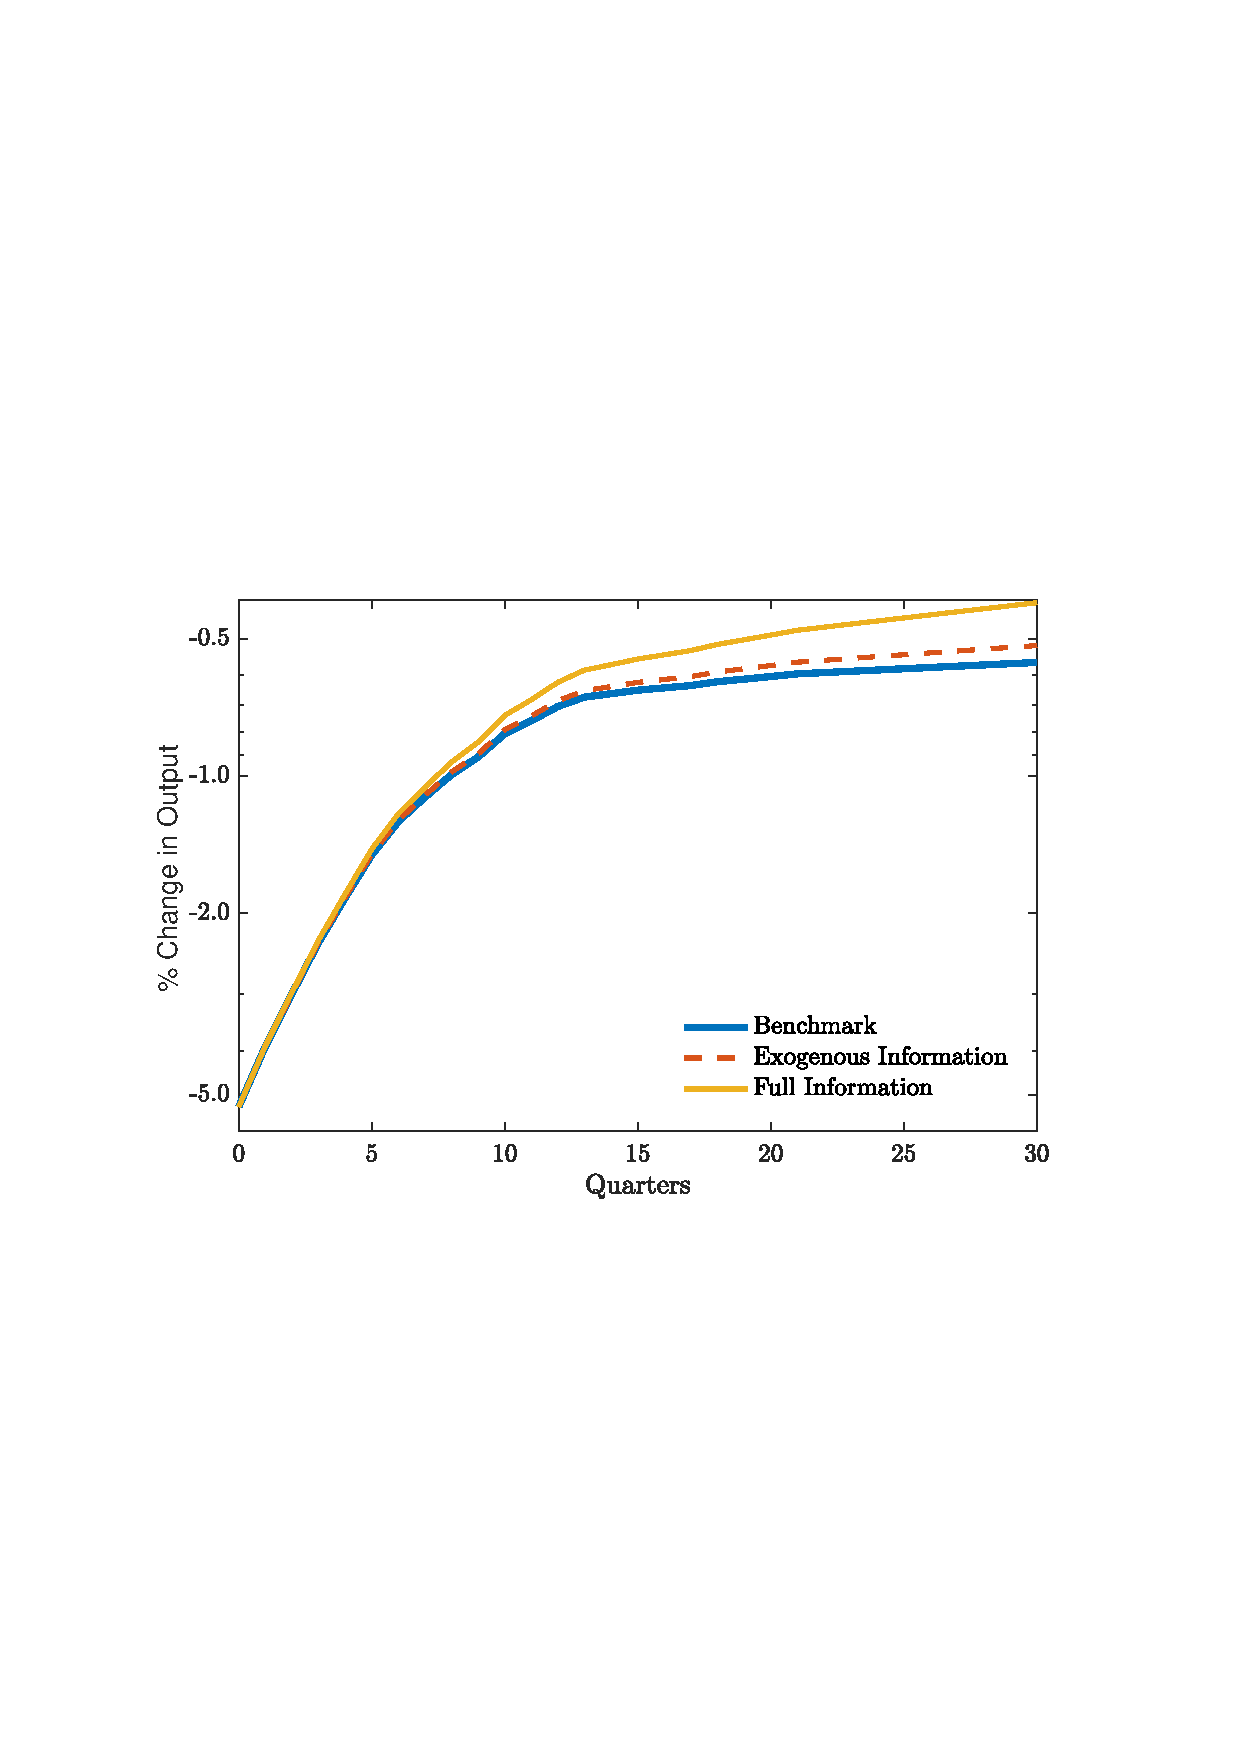
\includegraphics[width=\linewidth,trim=60 250 60 280,clip]{_input/figure_IRF_y2.pdf}
        %\label{fig:c}
    \end{subfigure}
    \hfill
    \begin{subfigure}{0.49\textwidth}
        \centering
        \caption{Investment}
        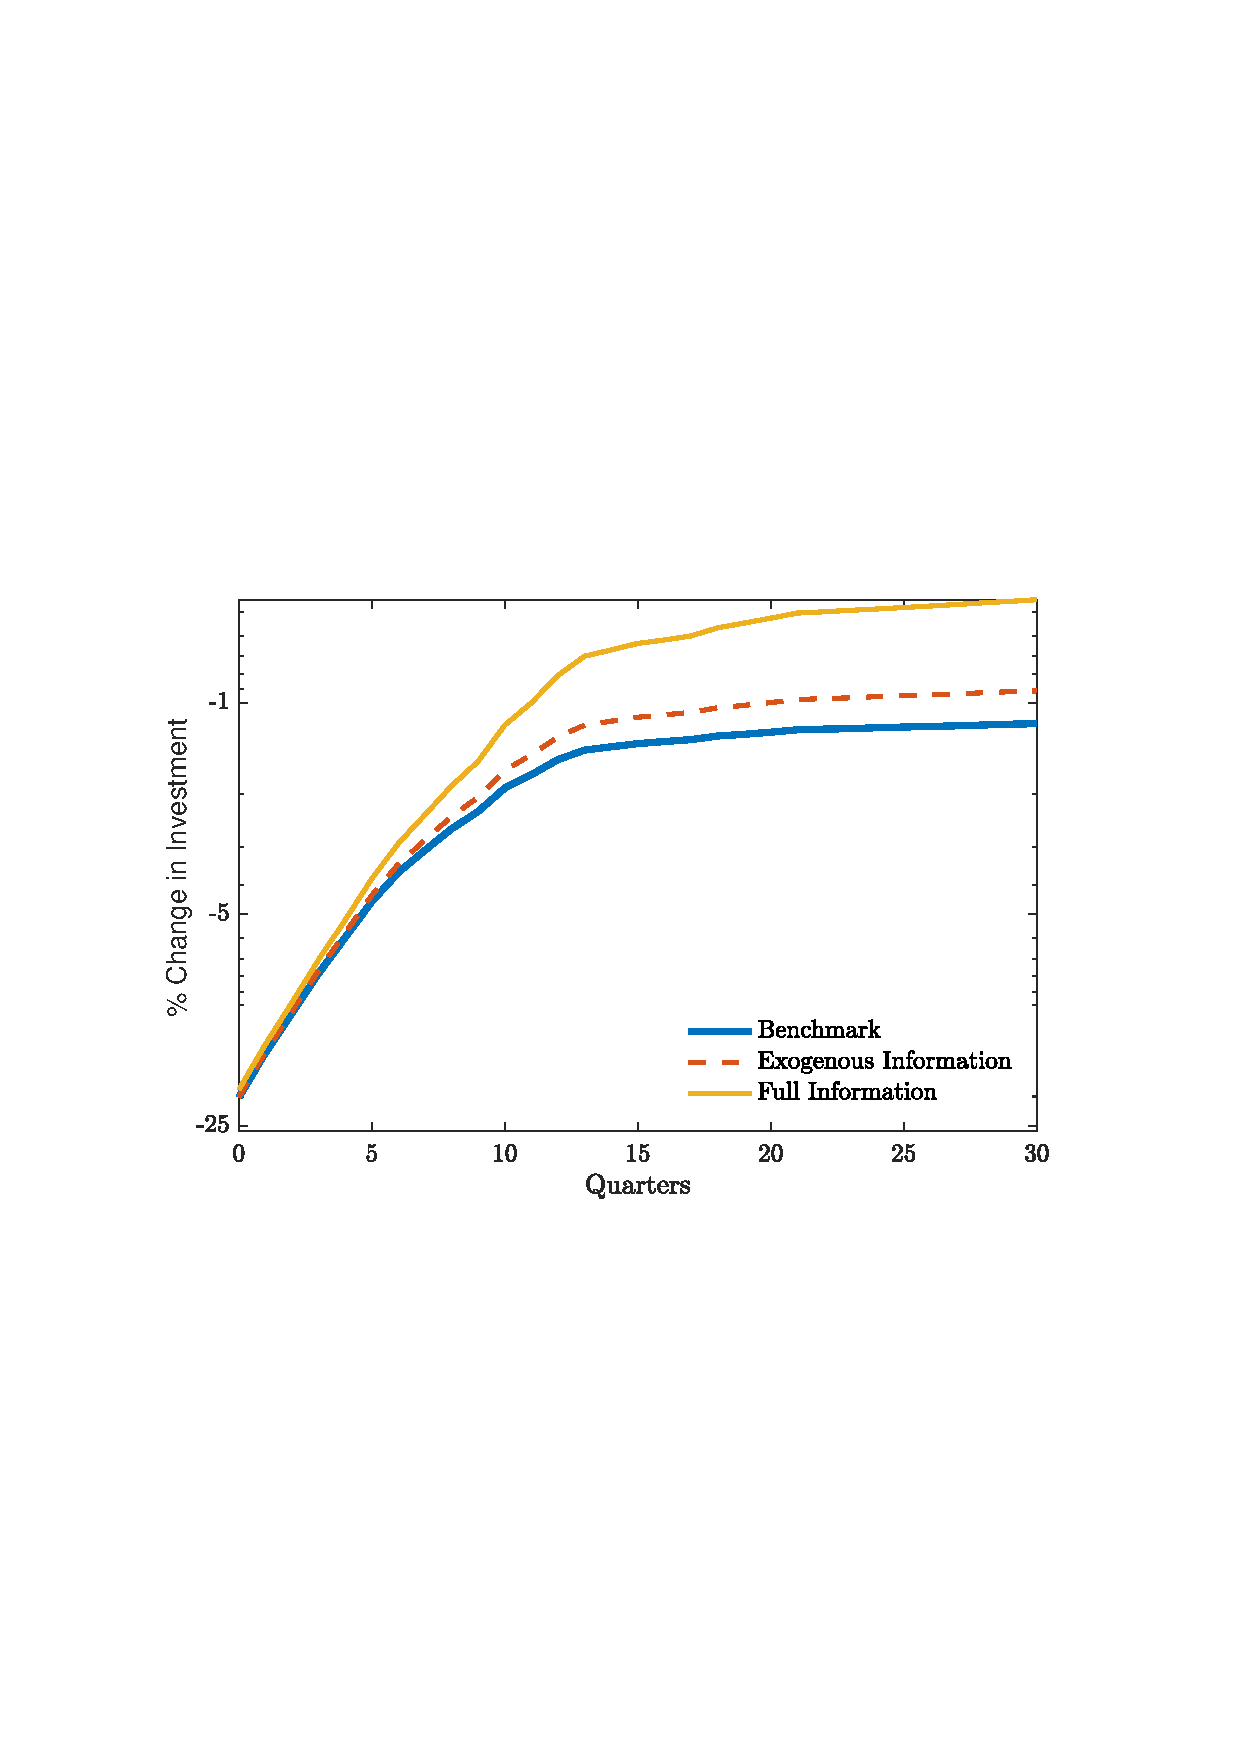
\includegraphics[width=\linewidth,trim=60 250 60 280,clip]{_input/figure_IRF_inv2.pdf}
        %\label{fig:b}
    \end{subfigure}		    
		\end{center}
		\vspace{-0.39cm}
		\footnotesize
                {\protect\footnotesize \textit{Note:}
                  The figure shows impulse response functions to a negative productivity shock (transitioning from $z_h$ to $z_l$). Panels (b)-(d) show the responses of capital $K_t$, output $Y_t$, and investment $I_t$, respectively, while Panel (a) shows the underlying shock to the economy (productivity $z_t$). The horizontal axis refers to quarters after the initial shock, $t$. We plot the dynamics of our benchmark economy (solid blue line), the exogenous-information economy (dashed red line), and the full-information economy (solid yellow line).}
\end{figure}

Finally, Appendix \ref{app-tab:mean-biased-capital} illustrates the
non-linear relationship between aggregate volatility and the accuracy
of expectations about capital. Recall that a main driver of savings
differences caused by incomplete information was the resulting lack
of information about capital (Figure \ref{fig:4-savings-choices}).
To do so, we compare the business-cycle dynamics of the benchmark
economy with those from two additional economies, where households
\emph{exogenously} learn the current capital stock with a fixed probability
every period, in addition to their \emph{endogenous} decision to acquire
information about productivity. Our results document strong non-linearities
in the effects of incomplete information: In the case in which household
learn capital every period\textemdash and thus for which only \emph{static
effects }of incomplete information about productivity exists\textemdash the
volatility of capital increases by around 5 percent relative to the
full-information case. By contrast, if households learn capital every
10 quarters, this difference is more than 2.5 as large\textemdash while,
in our benchmark model, where households are never exogenously told
about the capital stock, volatilities increase by close to a factor
of 4. Our results, thus, highlight the important role of dynamic information
accumulation about the capital stock, and the strong non-linearities
inherent in the business-cycle effects of mean-biased capital expectations.

We conclude that the presence of heterogeneous information serves
as an amplifying force\textemdash it induces weaker mean-reversion
of the capital stock relative to the full-information case. This amplification
acts as a powerful propagation mechanism, making the economy respond
more to shocks than standard full-information models would otherwise
predict.\footnote{These dynamics elucidate a more general feature of our framework:
Information acquisition choices are \emph{strategic substitutes. }The
individual benefits of information rise with the volatility of the
capital stock. But, when the average share of information in the economy
increases, the volatility of the capital stock falls, and so does
the incentive to acquire information. In previous work, \citet{BKKS_2},
we show how this may imply non-existence of homogeneous-information
(representative-agent) equilibria in neoclassical economies.}

\subsection{Amplification and the Wealth Distribution \label{subsec:Amplification-and-the}}

In the previous section, we showed that heterogeneous information
amplifies business cycles. The strength of resulting amplification
yet depends centrally on the shape of the wealth distribution. Because
uninformed savings are more procyclical for the bottom 80 percent
of the wealth distribution but countercyclical for the rich, the distribution
of capital holdings determines the strength of the amplification.
The more of the capital stock that is held by households whose uninformed
savings are more procyclical, the larger the amplification. 

Table \ref{tab:moments} addresses the empirical validity of our
results. The table shows the wealth distribution in the data and in
our benchmark economy, as well as the associated consumption expenditure
shares, the flip-side of savings. Although there are well-known issues
related to the lack of skewness in wealth with the Aiyagari-Bewley-Huggett-Imrohoroglu
class of models that we depart from (see Section \ref{sub-sect-ext:cost}),
on balance, the benchmark model does well at capturing the salient
dimensions of the joint distribution of consumption and wealth. 
\begin{table}[t]
\textcolor{black}{\caption{Selected Variables by Wealth: Data vs Model (\% share of)}
\label{tab:moments}}

\textcolor{black}{\vspace{-0.22cm}}

\textcolor{black}{\def\sym#1{\ifmmode^{#1}\else\(^{#1}\)\fi}

\centering
\begin{tabular*}{0.98\textwidth}{@{\extracolsep{\fill}}lrrrrrrrr@{}}
\toprule \toprule
 & \multicolumn{4}{c}{Benchmark Model} & \multicolumn{4}{c}{Entrepreneur Model} \\
\cmidrule(lr){2-5}\cmidrule(lr){6-9}
& \multicolumn{2}{c}{Wealth} & \multicolumn{2}{c}{Expend.} & \multicolumn{2}{c}{Wealth} & \multicolumn{2}{c}{Expend.} \\
\cmidrule(lr){2-3}\cmidrule(lr){4-5}\cmidrule(lr){6-7}\cmidrule(lr){8-9}
NW & Data & Mod & Data & Mod & Data & Mod & Data & Mod \\
\midrule
$D1$ & -0.8 & 0.9 & 6.9 & 7.6 & -0.8 & -0.2 & 6.9 &  7.4\\
$D2$ &  0.0 & 2.1 & 4.3 & 8.3 & 0.0  &  0.5 & 4.3 &  7.8\\
$Q2$ & 1.1  & 7.4 & 13.7 & 17.5 & 1.1 & 2.8 & 13.7 &  16.0\\
$Q3$ & 5.2 & 12.9 & 17.8 & 18.7 & 5.2 & 5.5 & 17.8 & 16.7\\
$Q4$ & 14.6 & 22.0 & 22.5 & 20.6 & 14.6 & 10.5 & 22.5 & 17.9 \\
$Q5$ & 79.9 & 54.8 & 34.7 & 27.3 & 79.9 & 80.8 & 34.7 & 34.2\\
\bottomrule \bottomrule
\end{tabular*}

\vspace{0.22cm}}

\footnotesize{\textit{Note:} The table shows the distribution of wealth and expenditures from the U.S. Panel Study of Income Dynamics (\citealp{data_psid}). The wealth shares in the SCE (2014-2022) are similar to those in the PSID. }
\end{table}

The table shows that a sizable share of consumption occurs for households
for which the presence of incomplete information has bite. In the
benchmark model, 52\% of consumption expenditures are made by households
in the bottom 60\% of wealth, whose uninformed savings are more procyclical.
Another 27\% occur for households above the 80th percentile, where
countercyclical forces operate for the wealthiest. A substantial share
of consumption expenditures thus occur for households in the region
of the distribution for which the presence of incomplete information
has bite on their consumption-savings choices (Figure \ref{fig:4-savings-choices}). 

Crucially, the net effect\textemdash business-cycle amplification\textemdash here
arises because (i) households with little or moderate wealth, whose
uninformed savings are more procyclical, control a large share of
consumption-savings; and (ii) rich households acquire information
frequently enough to neutralize most of their potential dampening
effect. This insight has important implications: In Section \ref{subsec:Matching-the-Wealth},
we document that even when we extend our model framework to better
match wealth concentration at the top, business-cycle amplification
remains the dominant feature, as the poor and middle class still control
substantial resources and acquire information infrequently. We conclude
that the amplification documented in Section \ref{subsec:aggregate-implications}
provides a suitable first-pass guide to the business-cycle consequences
of heterogeneous information. 

\subsection{Distributional Implications\label{subsec:Distributional-Implications}}

We next turn to the distributional implications of heterogeneous incomplete
information. The wealth distribution does not only affect the consequences
of heterogeneous information but is itself also affected by its presence.
Figure \ref{fig-6-dist-change} and Table \ref{tab:inequality-moments}
compare the wealth distribution in our calibrated benchmark economy\textemdash averaged
across a long simulation\textemdash with those from the equivalent
full-information and exogenous-information economies.

\begin{figure}
\caption{Information and the Wealth Distribution}
\label{fig-6-dist-change}\vspace{0.00cm}\vspace{0.00cm}\hspace{-1cm}
\begin{centering}
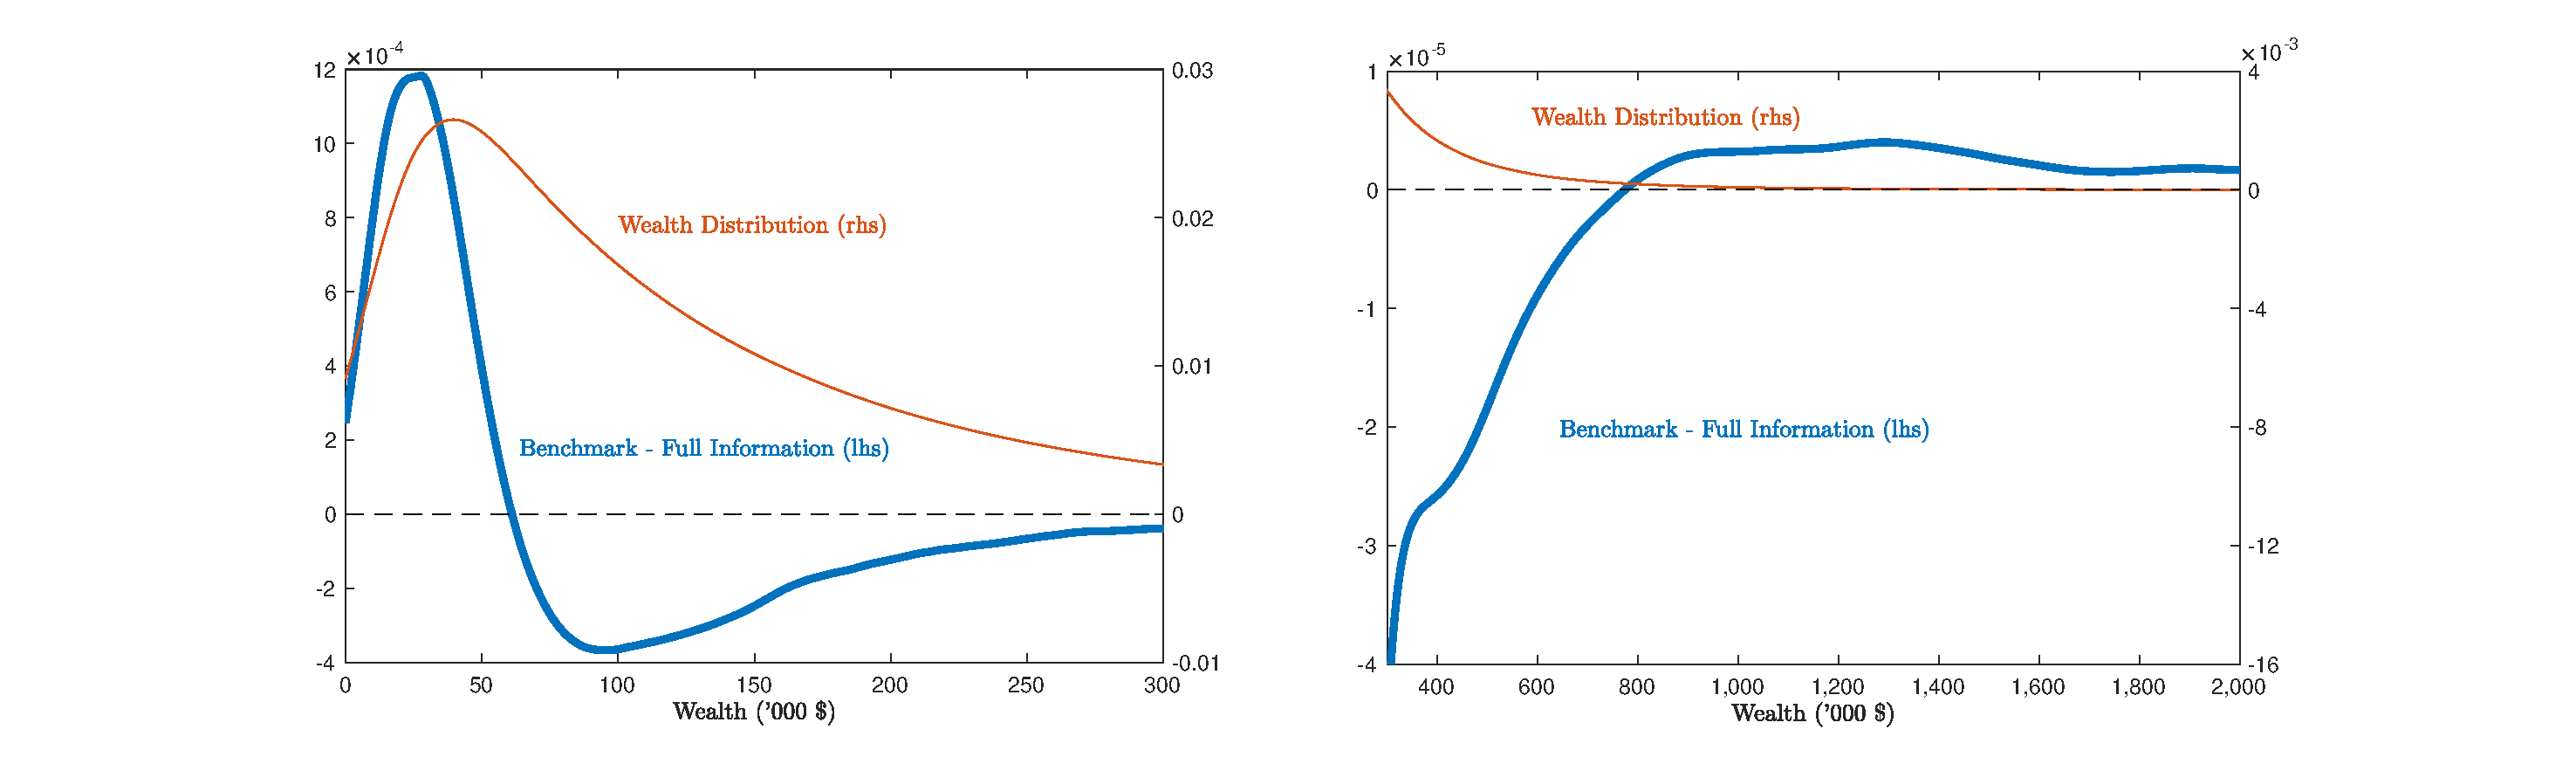
\includegraphics[viewport=150bp 0bp 1350bp 400bp,clip,scale=0.45]{_input/figure_8}
\par\end{centering}
\hspace{0.35cm} Panel (a): Distribution Differences (I/II)\hspace{1.55cm}
Panel (b): Distribution Differences (II/II)\vspace{0.29cm}

{\footnotesize\emph{Note}}{\footnotesize : The figure shows differences
in the wealth distribution relative to the full-information economy
(left-hand side axis) and plots the underlying wealth distribution
in the benchmark economy (right-hand side axis). The horizontal axis
is household wealth (capital levels) in USD '000 (\$). We use 2020
values of U.S. household income to convert values in the model to
\$ amounts. Probability density functions are estimated from a simulated
panel of households, using a kernel density estimator with the Epanechnikov
kernel.}{\footnotesize\par}
\end{figure}
\begin{table}[t]
\caption{Wealth Distribution}

\label{tab:inequality-moments}
\begin{centering}
\textcolor{black}{\def\sym#1{\ifmmode^{#1}\else\(^{#1}\)\fi}

\begin{tabular*}{0.99\textwidth}{{l C{1.97cm} C{1.97cm} C{1.97cm} C{1.97cm} C{1.97cm}}}
\toprule \toprule\\[-1.8ex]
& \multicolumn{5}{c}{Panel (a): Level of Moments}\\
&  Gini G& $90/10$ & $99/1$ & $90/50$ &$\text{Cor}(K,Y )$ \\
\cline{2-6} \\[-1.8ex]
Benchmark Model                   & 0.51 & 14.53 & 345.3 & 3.51 & 0.62\\ 
[1em] Exogenous Information & 0.51 & 14.51 & 339.3 & 3.45 & 0.56\\ 
[1em] Full  Information            & 0.50 & 14.15 & 327.8 & 3.39 & 0.49\\ 
\hline
&&&\\
& \multicolumn{5}{c}{Panel (b): Percent  Difference w.r.t. Full Information} \\ 
&  Gini G & $90/10$ & $99/1$ & $90/50$  &$\text{Cor}(K, Y)$ \\
\cline{2-6}\\[-1.8ex]
Benchmark Model & 1.72 & 2.74 & 5.35 & 3.75 & 24.67\\ 
[1em] Exogenous Information & 1.17 & 2.57 & 3.51 & 1.79 & 14.39\\ 
\bottomrule
\bottomrule
\end{tabular*}
}
\par\end{centering}
\vspace{0.22cm}

{\footnotesize\emph{Note}}{\footnotesize : The table shows the mean
of the logarithm of capital ($K$), the Gini coefficient of the capital
distribution ($G)$, as well as the 90/10, 99/1, and 90/50 percentile
ratios of the wealth distribution. In addition, the table shows the
correlation between the logarithm of capital and log. output ($Y)$
($\text{Cor}(K,Y)$). The table computes these moments in the calibrated
model (``Benchmark Model''), the associated full-information economy
(``Full Information''), as well as in the model with an exogenously
specified probability of acquiring information (``Exogenous Information'').
The probabilities of information acquisition in the benchmark model
are, on average, 0.122 and 0.097, respectively, for the unemployed
and employed. This probability is set equal to 0.10 in the exogenous-information
case for all households and for all moments in time.}{\footnotesize\par}
\end{table}

The introduction of heterogeneous incomplete information increases
wealth dispersion relative to the full-information case\textemdash with
more mass placed at the bottom and at the top of the wealth distribution
(Panel (a) and (b) in Figure \ref{fig-6-dist-change}). Conversely,
there are fewer households with intermediate wealth levels (between
\$65,000-750,000). Consistent with the widening of the wealth distribution,
all measures of inequality (Gini coefficient, the 90/10-ratio, as
well as the 99/1-ratio) increase modestly between 2-5 percent (Table
\ref{tab:inequality-moments}). Finally, comparing instead to the
exogenous-information case, the widening of the wealth distribution
is also somewhat amplified: Households\textquoteright{} endogenous
information choices increase the widening of the wealth distribution,
especially near the top.\footnote{The introduction of heterogeneous information also causes the dynamics
of inequality to change, increasing its volatility over time. We analyze
the dynamics of inequality in depth in Appendix \ref{subsec:inequality-dynamics}.}

Underlying these modest overall increases in inequality are\emph{
substantially larger but offsetting} gross effects. In Appendix \ref{app-sub-sec:wealth-decomp},
we decompose the overall change in the wealth distribution into three
separate forces: (i) the presence of incomplete information; (ii)
the heterogeneity that exists in information choices; and (iii) the
change in the equilibrium law of motion. Combined, these three forces
capture the partial and general equilibrium channels by which heterogeneous
incomplete information itself alters the wealth distribution.

The main driver of the overall increase in inequality is the presence
of \emph{incomplete information}. Uninformed households make savings
errors that, while individually rational, introduce dispersion in
wealth accumulation. The more procyclical savings of low-to-medium
wealth uninformed households\textemdash combined with the more countercyclical
savings of rich uninformed households\textemdash amplify inequality:
Poor uninformed households save less precisely when returns are high,
while wealthy households are unable to effectively run down wealth
to increase consumption. In effect, the presence of incomplete information
increases the ``randomness'' of savings choices across the wealth
distribution. This parallels the mechanism in \citet{piketty2003income},
who show that random savings rates combined with linear policy functions
can generate Pareto tails in the wealth distribution. In our framework,
however, this randomness is micro-founded through rational information
choice rather than assumed exogenously.\footnote{That said, because the magnitude of the errors are comparatively small
relative to what is needed, in the benchmark model this force is not
sufficiently potent to generate a thick Pareto tail of wealth (cf.
Section \ref{subsec:Matching-the-Wealth}).}

While the presence of incomplete information widens the distribution,
the other two forces dampen the increase. First, the \emph{heterogeneity
in information choices} allows the most exposed households\textemdash the
poor unemployed and the wealthy\textemdash to acquire information
at higher rates, reducing their savings errors, all else equal. Second,
the \emph{weakened mean-reversion of capital} (apparent in the change
in the equilibrium law of motion) increases the persistence of wages
and returns, strengthening income effects that compress the distribution.
On balance, we find that the former effect quantitatively dominates
the latter, leading to a modest overall increase in inequality (Table
\ref{tab:inequality-moments}). The combined effects of heterogeneous
information are subtle\textemdash and, crucially, affect different
parts of the distribution differentially.\footnote{Notice that while heterogeneity in information acquisition by itself
decreases inequality, our benchmark economy features more inequality
than its exogenous information counterpart (Table \ref{tab:inequality-moments}).
This is due to the weaker general equilibrium dynamics in our benchmark
model with heterogeneous information.}

\subsection{Matching the Wealth Distribution\label{subsec:Matching-the-Wealth} }

A prominent issue with the Aiyagari-Bewley-Huggett-Imrohoroglu class
of models that we depart from is that it does not generate realistic
wealth heterogeneity: The data display significantly more skewness
than the models. Although the presence of stochastic death helps match
the lower-tail of the wealth distribution, the concentration of wealth
among the richest is likewise too small in our benchmark framework.
The Gini coefficient is as a result too low: On the basis of the 2022
SCF, the Gini coefficient on wealth in the U.S. is around 0.80. In
the benchmark model, by contrast, the equivalent number is only 0.51.
The presence of heterogeneous information, as argued above, modestly
increases wealth concentration among the rich\textemdash and thus
the Gini coefficient\textemdash but does not do so by enough to match
the data.

One of the main purposes of our line of research is to extend heterogeneous-agent
frameworks to simultaneously allow for heterogeneity in wealth and
expectations. It therefore seems important to ensure that the forces
we highlight extend to models that roughly match the observed wealth
distribution\textemdash especially given how the amplification that
we document depends on it. To analyze such an environment, Appendix
\ref{app-subsec-wealthy} follows \citet{bayer2024shocks} and extends
our baseline framework with a CES-structure for final production and
a share of entrepreneurs in the population, who do not work but earn
all pure rents in the economy. We set the share of entrepreneurs to
1 percent and the elasticity of substitution to target the top 10
percent wealth share. We also allow households to borrow (up to $k_{\min}<0$),
so as to match the negative wealth share held by the bottom of the
distribution; and follow \citet{bayer2024shocks} and set the transition
matrix governing switches between worker and entrepreneur states to
the estimated values in \citet{guvenen2014risky}. Finally, we recalibrate
the information cost parameters to target the same forecast error
moments as our benchmark framework. Table \ref{tab:moments} shows
that the extended model matches closely the wealth distribution in
the data.\footnote{While the model better matches the Gini coefficient on wealth, it
is, however, not able to match the Pareto tail of wealth in the data,
as the wealth distribution merely inherits the tail of entrepreneurial
earnings (\citealp{benhabib2018skewed}). We also modestly increase
$\mu$ to 0.45, to better target recent U.S. values.}

Figure \ref{fig:app-1-unemployment-errors} compares the accuracy
of unemployment forecasts across the wealth distribution with that
in the benchmark model. Although the inverse u-shaped relationship
is slightly shallower compared to that in the benchmark model, the
overall strength of the relationship is similar to before. Consistent
with this similarity, Table \ref{tab:robust} and \ref{app-tab:extended-model-moments}
show that the presence of heterogeneous information once more amplifies
business cycles: The standard deviation of capital and output, for
example, increases by 71 percent and 9 percent, respectively. This
compares to 64 percent and 11 percent, respectively, in the benchmark
model. This resemblance is not obvious ex ante. With more wealth concentrated
at the top, one might expect wealthy uninformed households' countercyclical
savings to \emph{dampen} rather than \emph{amplify} fluctuations.
Table \ref{tab:moments} helps explain why this does not occur. Despite
greater concentration, the bottom 60 percent still account for a substantial
share of consumption expenditures (and exhibit the strongest procyclical
bias when uninformed). Additionally, wealthy households still acquire
information at high rates, and the extended model further introduces
negative-wealth households whose procyclical uninformed savings counters
those from wealthy entrepreneurs.

Finally, Table \ref{tab:robust} and \ref{app-tab:extended-model-moments}
show that, as in our benchmark framework, the presence of incomplete
information once more widens the wealth distribution, especially the
right tail, while the modified general equilibrium dynamics, all else
equal, dampens the increase. The presence of heterogeneous incomplete
information, as such, causes the Gini to increase by 8.6 percent.\footnote{One noteworthy difference between our benchmark framework and the
entrepreneur extension is that, while in the former case heterogeneity
in information choices dampened the overall increase inequality, in
the latter case it contributes to the widening of the wealth distribution
(Table \ref{app-tab:wealth-dist-decomposition-entrepreneur}). This
once more shows that the details of who acquires information matters
for inequality.}\textcolor{orange}{{} }The increased randomness in savings choices caused
by incomplete information operates on a more skewed distribution,
amplifying the dispersion of wealth at both tails.

Overall, we conclude that the consequences of heterogeneous incomplete
information that we highlighted above extend to a framework which
better matches the top and bottom of the wealth distribution. Clearly,
the addition of another source of heterogeneity\textemdash whether
households are workers or entrepreneurs\textemdash further complicates
the already intricate consequences of heterogeneous incomplete information.
Yet, the overall consequences that we find are qualitatively and quantitatively
similar and akin to those in our benchmark framework.

\subsection{Discussions and Robustness}

Before ending with a policy exercise that targets the wealth-expectation
nexus, we briefly turn to several alternative versions of our benchmark
framework. The overall aim is to demonstrate that our main findings\textemdash amplified
business cycles and modest increases in inequality\textemdash are
robust to alternative assumptions about information costs and the
cyclicality of taxes. We recalibrate all alternative models to target
the same capital-output ratio and (where appropriate) average errors
as our benchmark model. Table \ref{tab:robust} summarizes the results.

\begin{table}[t]
\caption{Summary of Robustness Exercises}

\textcolor{black}{\label{tab:robust}\vspace{-0.22cm}}

\begin{centering}

\textcolor{black}{\def\sym#1{\ifmmode^{#1}\else\(^{#1}\)\fi}

\begin{tabular*}{0.98\textwidth}{l C{2.00cm} C{2.00cm} C{2.00cm} C{2.40cm}}
\toprule \toprule
\\[-6pt]
& \multicolumn{4}{c}{Panel (a):  Difference \% to Alternative Model} \\[3pt]
 & $\sigma(K)$ & $\sigma(Y)$ & Gini & Reference \\
\midrule 
Full Information w/o  Costs & $-0.02$ & $-0.00$ & $-0.28$ & Tables~\ref{tab:business-cycle-moments-angelvsdemon},~\ref{tab:inequality-moments-angelvsdemon} \\
Exo. Information w/o Costs  & $-0.04$ & $-0.01$ & $-0.28$ & Tables~\ref{tab:business-cycle-moments-angelvsdemon},~\ref{tab:inequality-moments-angelvsdemon} \\
Scaled Utility Cost        & $-1.77$ & $-0.52$ & $-0.19$ & Table~\ref{app-tab:monetary-cost-endo-1} \\
No Resource Cost        & $-18.49$ & $-5.10$ & $-1.48$ & Table~\ref{app-tab:monetary-cost-endo} \\
%Internalized $K$ Uncertainty & 28.8 & 4.9  & 4.3 & Table~\ref{app-tab:sigK-model-moments} \\
\\[-6pt]
\midrule
\\[-6pt]
& \multicolumn{4}{c}{Panel (b): Difference \% to Full Information Model} \\[3pt]
 & $\sigma(K)$ & $\sigma(Y)$ & Gini & Reference \\
\midrule
Benchmark Model          & 64.3 & 11.0 & 1.7 & Tables~\ref{tab:business-cycle-moments},~\ref{tab:inequality-moments} \\
Acyclical Taxes               & 66.1 & 7.7  & 1.9 & Tables~\ref{tab:business-cycle-moments-acyc},~\ref{tab:inequality-moments-acyc} \\
Entrepreneur Model         & 71.0 & 9.0  & 8.6 & Table~\ref{app-tab:extended-model-moments} \\
\bottomrule \bottomrule
\end{tabular*}
}

\end{centering}

\vspace{0.38cm}

{\footnotesize\emph{Note}}{\footnotesize : Panel (a) reports the difference
in moments relative to the relevant alternative economy, isolating
the effect of each assumption; Panel (b) instead shows the change
relative to a specifications full-information counterpart. $\sigma(K)$
and $\sigma(Y)$ denote the standard deviations of the log. of capital
$K$ and output $Y$, respectively. ``W/o Costs'' refers to the alternative
economies in which information is freely available (Appendix \ref{app-subsec-resource-cost-information}). }{\footnotesize\par}
\end{table}


\paragraph*{Angels and Demons:\label{sub-sect-ext:cost}}

The frameworks considered so far with a fixed probability of information
acquisition keep the costs of information acquisition from the benchmark
model unchanged. Thus, while households have no choice about information
acquisition in these alternative models, they still have to pay the
resource and utility cost of information upon becoming informed. This
focuses any comparison between the different models on the \emph{endogeneity}
and \emph{incompleteness} of information itself\textemdash rather
than the size of costs associated with it. We relax this assumption
in Appendix \ref{app-subsec-resource-cost-information}, where we
instead make information freely (but randomly) available. We note
that the exogenous-information economy without information costs is
similar to the ``Mankiw-Reis''-style economy studied in \citet{auclert2020micro}
and \citet{carroll2020sticky}. Table \ref{tab:business-cycle-moments-angelvsdemon}
and \ref{tab:inequality-moments-angelvsdemon} show that key moments
change little irrespective of whether the given information is from
a ``Calvo-Angel'' or a ``Calvo-Demon''.\footnote{An anonymous referee provided the labeling for these alternative economies:
When we make information freely available in the alternative frameworks
with an (exogenously) pre-specified probability of information acquisition
it is as-if households are touched by a ``Calvo-Angel'' upon becoming
informed. By contrast, in the alternative frameworks that we studied
above, where households still have to pay the costs of information
upon becoming informed, it is as-if households are instead touched
by a ``Calvo-Demon''.} Business cycle moments are next to unaffected: The maximum difference
is less than a quarter of 1 percent (Table \ref{tab:business-cycle-moments-angelvsdemon}).
Inequality measures are slightly more affected, because the absence
of a resource cost affects the disposable income of the poor (Table
\ref{tab:inequality-moments-angelvsdemon}). Nevertheless, the maximum
difference in inequality measures is still below 1 percent. We conclude
that assumptions about the information costs themselves matter little
for the above comparisons between our benchmark economy and the alternative
informational environments.

\paragraph*{Homotheticity of Information Costs:\label{sub-sect-ext:cost-2} }

Our benchmark model features both a resource cost $\eta$ and a utility
cost $\kappa$ of information acquisition. Appendix \ref{app-subsec-c2-1}
explores the consequences that the non-homotheticity embedded in both
have for our results. First, making the utility cost homothetic\textemdash by
scaling it with the utility value of cash-at-hand\textemdash has only
negligible effects. Figure \ref{fig:app-unemployment-errors-scaled-ucost}
shows that the relationship between the accuracy of unemployment expectations
and wealth is nearly identical to that in the benchmark model\textemdash with
only a small increase in the size of the inverse u-shape noticeable.
Consistent with these findings, Table \ref{app-tab:monetary-cost-endo-1}
shows that the business-cycle and inequality statistics also do not
depend much on the non-homotheticity of the utility cost. The maximum
difference between our benchmark model and the moments of the model
with the scaled utility cost is less than 2 percent. By contrast,
the resource cost matters more. Removing it entirely dampens both
the amplification and the increase in inequality (Table \ref{app-tab:monetary-cost-endo})
documented above, and\textemdash importantly\textemdash eliminates
the inverse u-shaped relationship between accuracy and wealth in the
model (Figure \ref{fig:app-unemployment-errors-mon-cost}). Although
the information policy function still shows non-monotonicities similar
to those in the benchmark model, the resource cost, though small (roughly
0.1 percent\textcolor{violet}{{} }of average quarterly earnings), acts
as a barrier for wealth-poor households' information acquisition.
We conclude that the non-homotheticity embedded in the resource cost
of information is an important feature for matching the survey data\textemdash and
for the consequences of heterogeneous information highlighted above\textemdash unlike
the non-homotheticity implied by the utility cost.

\paragraph*{Cyclicality of Taxes:}

Following \citet{KS98} and others, our baseline framework assumes
a balanced government budget in every period (Section \ref{subsec:Government-Policy}).
Because the labor endowment falls and government outlays for unemployment
insurance rise in recessions, a balanced budget, however, implies
\emph{countercyclical tax rates}. To analyze the importance of these
for our results, Appendix \ref{app-sub-sec:acycl-taxes} studies an
alternative tax scheme in which the government perfectly smoothes
taxes through an implicit insurance scheme with (unmodelled) financial
intermediaries from the rest of the world. This follows the approach
taken in \citet{mitman2015optimal}, among others. In particular,
the government charges a constant tax rate $\tau^{\star}$ such that
the present value of labor-income taxes equals that of unemployment-benefit
payments when appropriately discounted.\footnote{The exact formula for the constant tax rate is $\tau=\mathbb{P}[z=z_{l}]\frac{\mu u_{l}}{u_{l}\mu+(1-u_{l})}+\mathbb{\mathbb{P}}[z=z_{h}]\frac{\mu u_{h}}{u_{h}\mu+(1-u_{h})}$,
where $\mathbb{\mathbb{P}}[z=z_{l}]$and $\mathbb{P}[z=z_{h}]$ are
the unconditional probabilities of a bust and a boom, respectively.} As expected, aggregate volatility is lower with acyclical taxes (Table
\ref{tab:robust} and \ref{tab:business-cycle-moments-acyc}); however,
crucially, relative to the full-information case, the increase that
arises due to heterogeneous incomplete information is similar to before.
The standard deviation of output, for example, increases by 8 percent
compared to 11 percent previously. While the equilibrium level of
inequality is similarly slightly smaller, the increase that arises
is, if anything, now somewhat larger\textemdash with a similar decomposition
of the overall increase to that from before. The 99/1-ratio, for example,
now rises by 7 percent versus 5 percent previously (Table \ref{tab:inequality-moments-acyc}).
We conclude that our main business-cycle and inequality implications
are robust to changes in assumptions about the cyclicality of income
taxes.

\medskip

Across all extensions, a consistent pattern emerges: Heterogeneous
information amplifies business-cycle volatility and modestly increases
inequality. The specific magnitudes vary\textemdash the resource cost
of information matters more for matching the empirical expectation
patterns, while the cyclicality of taxes and the homotheticity of
utility costs less\textemdash but the core mechanisms persist. Whether
households face cyclical or constant taxes, or operate in economies
with utility or resource costs for information, the fundamental two-way
relationship between wealth and information systematically alters
macroeconomic dynamics. Combined with the entrepreneur extension,
this robustness strengthens confidence that our conclusions reflect
genuine features of the wealth-expectation nexus rather than artifacts
of particular modeling choices.\textcolor{orange}{{} }The next section
shows how the interplay between information choice, (pre-cautionary)
savings, and the aggregate economy similarly modifies the effects
of a simple economic policy that targets inequality but has unintended
consequences due to the wealth-expectation nexus.

\section{Macroeconomic Policies and the Wealth-Expectations Nexus\label{sec:policy-experiment}}

The previous section documented the macroeconomic consequences of
the wealth-expectation nexus. Our findings raise a natural question:
Do macroeconomic policies have important additional effects through
the wealth\textendash expectation link? We close the paper by illustrating
the potential for such consequences using a simple policy experiment
that directly affects a group with high information acquisition rates.
Specifically, we consider a 10 percentage points increase in the replacement
rate from unemployment $\mu$ (from 40 to 50 percent of wages).\footnote{We abstract from any micro or macro effects on search effort or vacancy
posting \citep[see, e.g.,][]{karahan2025micro,hagedorn2013unemployment}.} The unemployed poor are the second category of households (along
with the rich) that we identified as acquiring information at higher
rates than the average (Section \ref{subsec:information-choice}).
Table \ref{tab:re-rate-moments} and Figure \ref{fig-6-dist-change-reprate}
in the Appendix report the macroeconomic consequences.

The increase in unemployment benefits\textemdash combined with the
increase in labor-income taxes required to finance them\textemdash reduces
the income risk from unemployment, and thus both the incentive to
accumulate precautionary savings and to acquire information about
the current state of the economy. As such, the immediate effect of
the rise in benefits is to reduce aggregate savings by 1.5 percent.
When the replacement rate is increased, the unemployed especially
reduce both their savings and their rate of information acquisition,
the latter by close to 13 percent.\footnote{Since there are fewer unemployed than employed households, the average
probability of information acquisition across all households falls
by almost 3 percentage points.} This reduction in information acquisition decreases the accuracy
of expectations, dampens the mean-reversion of capital by increasing
the procyclicality of savings by the poor, and thus increases the
overall volatility of output (by 3.5 percent). In contrast, in the
full-information case, the volatility of output hardly changes (rises
only by 0.4 percent). Only the benchmark (endogenous-information)
economy generates substantial additional business-cycle amplification
through the information channel (Table \ref{tab:re-rate-moments}
and Appendix \ref{app-sec:Counterfactual-Policy-Experiment}).

The effect of the increase in unemployment benefits on inequality
is similarly surprising: The Gini coefficient on wealth rises by 5.7
percent due to the increase in unemployment benefits, nearly twice
the increase under full information. The savings and information behavior
of the rich\textemdash for whom post-tax labor or replacement incomes
account only for a small share of total wealth\textemdash is nearly
unaffected \emph{directly} by the change in policy. Yet, because the
reduced precautionary savings by the poor increases returns to capital,
it increases the average savings of the rich. As the reduction in
information acquisition is further concentrated among the poor, their
reduction in savings is worsened by their inability to save when future
returns are high. The poor make larger errors precisely when opportunities
for wealth accumulation are greatest. This explains why the rise in
inequality documented in Table \ref{tab:re-rate-moments} and Figure
\ref{fig-6-dist-change-reprate} is substantially more pronounced
in the benchmark economy compared to the economies with full and (to
a lesser extent) exogenous information.
\begin{table}
\caption{Quantitative Effects of Increased Unemployment Benefits}

\label{tab:re-rate-moments}\textcolor{black}{\vspace{-0.22cm}}

\textcolor{black}{\def\sym#1{\ifmmode^{#1}\else\(^{#1}\)\fi}

\begin{tabular*}{\textwidth}{@{\extracolsep{\fill}} lcccccccc }
\toprule
\toprule
& $\mu(K)$ & $\sigma(Y) $ & Gini (G)  & $ 90/10 $ & $99/1$ & $90/50$ & $\text{Info U.}$ & $\text{Info E.}$\\
\midrule
Benchmark Model & -1.63 & 3.52 & 5.66 & 24.85 & 44.53 & 7.50 & -12.63 & -1.77\\ 
[1em] Exogenous Information & -1.32 & 1.06 & 4.66 & 23.73 & 40.24 & 6.48 & . & . \\ 
[1em] Full  Information & -0.99 & 0.36 & 3.25 & 22.47 & 33.86 & 4.71 & . & .\\ 
\bottomrule
\bottomrule
\end{tabular*}
}

\vspace{0.22cm}

{\footnotesize\emph{Note}}{\footnotesize : The table shows the effects
of a ten percentage-point increase in the replacement rate on moments
of the average cross-sectional capital distribution and the logarithm
of economy-wide output in percent. $\mu(K)$ denotes the mean of the
capital stock, while $\sigma(Y)$ denotes the standard deviation of
(log-)economy-wide output. The table computes the moments for the
both benchmark economy (``Benchmark Model'') and the associated
full-information and exogenous-information economies (``Full Information''
and ``Exogenous Information'', respectively). The final two columns
measure the percent difference in the average number of households
who acquire information. We compute this probability separately for
the employed and unemployed.}{\footnotesize\par}
\end{table}

The same results carry over to the extended environment of Section
\ref{subsec:Matching-the-Wealth}, which more closely matches the
wealth distribution (Appendix \ref{app-subsec-wealthy} and \ref{app-sec:Counterfactual-Policy-Experiment}).
An increase in unemployment benefits (i) \emph{increases} the volatility
of output, albeit slightly less so than in the benchmark model, due
to less wealth being held by the poor; and (ii) \emph{increases} inequality
by\emph{ more} after one accounts for households' endogenous information
choices. A policy designed to strengthen the safety net for the unemployed,
in essence, inadvertently reduces their incentive to be informed,
leading them to make larger savings errors that ultimately increase
inequality.

\medskip

While we above have abstained from making welfare statements about
the policy that we analyze, our positive findings indicate that policymakers
should proceed cautiously when evaluating the consequences of tax
and transfer policies. The effects on households\textquoteright{}
information choices may lead to implications that run counter to the
stated objectives\textemdash for example, their implications on wealth
inequality. For the case of an increase in unemployment benefits,
the endogeneity of household information choices acts to increase
inequality relative to standard full-information environments. More
generally, the above policy experiment illustrates that macroeconomic
policies may have important additional effects through changes in
the distribution of expectations: By changing the wealth distribution,
and hence distribution of agents\textquoteright{} information, macroeconomic
policies fundamentally alter an economy\textquoteright s responsiveness
to shocks. These additional effects, absent from standard full-information
environments, may be quantitatively important\textemdash both from
a positive and a normative perspective.

\section{Conclusion\label{sec:final-remarks}}

The frontier of macroeconomics continues to incorporate salient dimensions
of household and firm heterogeneity to provide a more complete and
accurate description of the macroeconomy. In this paper, we have illustrated
how the interaction between two important dimensions of household
heterogeneity\textemdash heterogeneity in expectations and heterogeneity
in wealth\textemdash gives rise to new qualitative and quantitative
insights about macroeconomic dynamics and the effects of macroeconomic
policies. In particular, we have demonstrated how the wealth-expectation
nexus increases the endogenous propagation of shocks and partially
accounts for the lack of inequality in standard frameworks with incomplete
markets. We have showed how the wealth-expectation nexus further fundamentally
alters the predictions of government policies such as unemployment
benefits\textemdash and in unexpected ways.

Our findings have important implications for both the heterogeneous-agent
macro literature and the literature on models with dispersed information.
For the former, our policy experiments provide a ``Lucas-style''
criticism (\citealp{lucas1976econometric}) to policy analysis in
incomplete-markets models: Any policy that has a substantial impact
on the wealth distribution will systematically affect household information
choices and their expectations, with associated consequences for macroeconomics
dynamics and the cross-section.\footnote{In this sense, our results provide a Lucas-style criticism (\citealp{lucas1976econometric})
of Lucas' own comments about the response of an economy with incomplete
information to shocks; that ``It seems safe and, for my purposes,
sensible to abstract here from the fact that in reality this situation
can be slightly mitigated by the purchase of additional information\textquotedblright{}
(p. 1121, \citealp{lucas1975equilibrium}). } For the latter, studying the consequence of dispersed information
in models with linear policy rules misses the important two-way interaction
between the distribution of agent wealth and the non-linearity of
the value of additional information. Our framework provides a laboratory
to push both strands of the literature forward to explore new questions
in macroeconomics.

Our analysis has been positive in nature but raises interesting normative
questions. In particular, information choices have obvious externalities
in our environment through the implied change in the dynamic properties
of prices and quantities. Does this mean policymakers should subsidize
information or alter the manner in which they condition their policy
instruments? Should such subsidies or policy instruments target a
particular subset of the population? And how close do market-based
or institutional solutions, which collect information on behalf of
households and distribute it to them, come to the constrained efficient
allocation? We leave these exciting questions for future research.

\newpage

% Data citations: the JPE requires every dataset used in the paper to appear
% in the reference list. Those cited in the text resolve on their own; the
% remainder are forced into the bibliography here.
\nocite{data_sce,data_spf,data_psid,data_cps,
        data_fred_cpiaucsl,data_fred_cpilfesl,data_fred_csushpinsa,
        data_fred_unrate,data_fred_prs85006023,data_fred_ce16ov,
        data_fred_cnp16ov,data_fred_fedfunds,data_fred_gdpc1,
        data_fred_a939rx0q048sbea,data_fred_a794rx0q048sbea,
        data_fred_nfirsaxdcusq,data_fred_rknanpusa666nrug}

\bibliographystyle{chicago}
\bibliography{literature}

\newpage


\appendix
\begin{center}
\section*{\Large{{\fontfamily{concmath}\selectfont  \textbf{Online Appendix for \\
``Expectation and Wealth Heterogeneity in the Macroeconomy}''}}}


\bigskip

Tobias Broer \quad Alexandre Kohlhas \quad Kurt Mitman \quad Kathrin Schlafmann \\

\bigskip

May 2026
\end{center}
\vspace{-0.29cm}
\appendixwithtoc

\section{Motivating Evidence\label{sec:appendix-a}}

\renewcommand\theequation{A\arabic{equation}} \setcounter{equation}{0}
\setcounter{subsection}{0}

\counterwithin{table}{section}

\counterwithin{figure}{section} 

\subsection{Additional Estimates}

\begin{table}[H]
\caption{Unemployment Expectations Across the Wealth Distribution}
\label{tab:a1-unemployment-errors}\textcolor{black}{\vspace{-0.22cm}}

\textcolor{black}{\def\sym#1{\ifmmode^{#1}\else\(^{#1}\)\fi}

\begin{tabular*}{\textwidth}{@{\extracolsep{\fill}} l c c c}
\hline\hline
& \multicolumn{3}{c}{\emph{Absolute Error}}\\
& (1)  & (2)  & (3) \\
\hline
Wealth Percentile (0-10)                  &  -0.009                  & 0.063\sym{***}   & 0.060\sym{***}\\
                                                         & (0.020)                  &(0.017)                & (0.017) \\
Wealth Percentile (10-20)                &  0.045\sym{**}      & 0.088\sym{***}   & 0.082\sym{***} \\
                                                         & (0.020)                  &  (0.018)              &  (0.017)  \\                                                               
Wealth Percentile (20-40)                & 0.064\sym{***}      & 0.089\sym{***}   & 0.084\sym{***} \\
                                                         &  (0.016)                 &(0.013)                &  (0.013)  \\                                                               
Wealth Percentile (40-60)                & 0.050\sym{***}      & 0.029\sym{**}     & 0.026\sym{**} \\
                                                         &  (0.015)                 & (0.012)               &  (0.012)  \\                                                                                                                              
Wealth Percentile (60-80)                & 0.003                    & 0.023\sym{*}      & 0.020\\
                                                        &  (0.015)                 &  (0.012)              &  (0.012)  \\
Wealth Percentile (80-100)              & --              & --               & --  \\
                                                               &                 &                  &     \\
\hline
Male                                                       & --              & -0.004                              & -0.004     \\
                                                               &                 &  (0.008)                            &   (0.008)  \\
 Education                                     & --             &   -0.072\sym{***}              & -0.072\sym{***}\\
                                                                &                &   (0.010)                           & (0.010) \\          
 Non-participation                           & --             &   0.019\sym{*}                  & 0.020\sym{*}\\
                                                                &                &   (0.011)                           & (0.011) \\       
 Age                                               & --             &   0.013\sym{***}               & 0.013\sym{***}\\
                                                                &                &   (0.002)                           & (0.002) \\     
 Age$^2$                                        & --             &   -0.0001\sym{***}               & -0.0001\sym{***}\\
                                                                &                &   (0.00002)                           & (0.00002) \\  
\hline
Time Fixed Effects                                  & $\times$             & \checkmark      &  \checkmark\\
[1em]  Pre-2020Q1                                  & $\times$              & $\times$      &  \checkmark \\
\hline
Observations  & 40,998    & 37,163  &  36,408 \\
F Statistic       & 6.12      & 409.58  & 355.06  \\
$R^2$            & 0.01        & 0.44  & 0.40  \\
\hline
\hline
\end{tabular*}
}

\vspace{0.22cm}

{\footnotesize\emph{Note}}{\footnotesize : Column (1) shows estimates
from a regression of the absolute value of individual unemployment
errors on the wealth bucket (decile/quintile) that the individual
respondent belongs to. Estimates are relative to the wealthiest households,
those in the 80-100 percentile of the wealth distribution. Column
(2) adds controls to the regression specification: the age, education
(college or not), labor market status, and sex of the respondent,
as well as time fixed effects. Column (3) shows estimates ``pre-covid'';
that is, before January 2020. Robust standard errors in parentheses.
Sample: 2013M10-2020M3. $*$ p<.1, $**$ p<.05, $***$ p<.01}{\footnotesize\par}
\end{table}

\begin{table}
\caption{Test for the Monotonicity of Regression Coefficients}

\label{tab:monotinicty-test}\textcolor{black}{\vspace{-0.22cm}}

\textcolor{black}{\def\sym#1{\ifmmode^{#1}\else\(^{#1}\)\fi}

\begin{tabular*}{\textwidth}{@{\extracolsep{\fill}} l c c }
\hline\hline\\[-1.8ex]
& \multicolumn{2}{c}{Unemployment Forecasts}\\
 &  Left-hand side   & Right-hand side  \\
\cline{2-3}
Figure 1    (Panel a and b)                                                   &  0.01   & 0.32      \\
[1em] Figure 1 (Panel c and d)                                        & <0.01  &  <0.01 \\
&& \\
& \multicolumn{2}{c}{Inflation Forecasts}\\
 &  Panel a (lhs)  & Panel a (rhs)  \\
 \cline{2-3}
Figure 2                      			         & >0.99 & 0.01 \\
&& \\
& \multicolumn{2}{c}{House Price Forecasts}\\
 &  Panel a (lhs)  & Panel a (rhs)  \\
 \cline{2-3}
Figure 2                      				& 0.09 & 0.03\\
&&\\
\hline
\hline
\end{tabular*}
}

\vspace{0.22cm}

{\footnotesize\emph{Note}}{\footnotesize : The table reports p-values
from the Likelihood Ratio test by \citet{silvapulle2005constrained}
of monotonically declining regression coefficients ($H_{0}:\text{monotonic decline}$)
against the alternative ($H_{A}:\text{non-monotinicty}$) using the
SCE data discussed in Section }{\footnotesize\textcolor{red}{2}}{\footnotesize .
Results are reported using 10,000 draws from a semi-nonparametric
Bollen-Stine bootstrap procedure. The figure and panel labels correspond
to those used in the main text.}{\footnotesize\par}
\end{table}

\begin{table}
\caption{Unemployment Expectations and Wealth Percentiles}

\label{tab:percentile-reg}\textcolor{black}{\vspace{-0.22cm}}
\begin{centering}
\textcolor{black}{\def\sym#1{\ifmmode^{#1}\else\(^{#1}\)\fi}

\begin{tabular*}{0.75\textwidth}{@{\extracolsep{\fill}} l c}

\\[-1.8ex]\hline 
\hline \\[-1.8ex] 
 & \multicolumn{1}{c}{\textit{Dependent variable:}} \\ 
\cline{2-2} 
\\[-1.8ex] & \textit{Absolute Error}  \\ 
\hline \\[-1.8ex] 
 Wealth Percentile & 0.113$^{*}$ \\ 
  & (0.069) \\ 
  & \\ 
 Wealth Percentile Squared & $-$0.162$^{**}$ \\ 
  & (0.067) \\ 
  & \\ 
 Constant & 1.237$^{***}$ \\ 
  & (0.015) \\ 
\hline \\[-1.8ex] 
Controls & $\checkmark$ \\
Observations & 40,998 \\ 
%Residual Std. Error & 1.015 (df = 40995) \\ 
F Statistic & 6.877$^{***}$ (df = 2; 40995) \\ 
\hline 
\hline 
\end{tabular*} 
}
\par\end{centering}
\vspace{0.22cm}

{\footnotesize\emph{Note}}{\footnotesize : The table shows estimates
from a regression of the absolute value of individual unemployment
errors on the wealth percentile that the individual respondent belongs
to, in addition to controls: the age, education (college or not),
labor market status, and sex of the respondent, as well as time fixed
effects. Robust standard errors in parentheses. Sample: 2013M10-2020M3.
\textasteriskcentered{} p<.1, \textasteriskcentered\textasteriskcentered{}
p<.05, \textasteriskcentered{} \textasteriskcentered{} \textasteriskcentered{}
p<.01}{\footnotesize\par}
\end{table}


\subsection{Data Construction\label{app:data}}

The SCE is a monthly internet survey of c. 1,300 ``household heads'',
defined as the person in a household who owns, is buying, or rents
the home. Subjects are chosen from the respondents to the Consumer
Confidence Survey (CCS), itself based on the universe of U.S. postal
addresses, to match demographic targets from the American Community
Survey, and remain in the survey for up to 12 months. The SCE core
module contains monthly information about households' expectations
about key macroeconomic and individual variables. Importantly, a yearly
module also asks the survey respondents for key financial variables,
including their financial wealth.\footnote{We match wealth observations with the household's monthly expectations
using the household's id variable. }

\subsubsection{Variable Definitions}

We focus on expectations of three variables: inflation, house prices,
and the unemployment rate. The former two ask respondents for their
best guess of a variable's outcome, in addition to the probability
of it falling into a number of bins. The exact questions are:
\begin{itemize}
\item Inflation:\\
``\emph{What do you expect the rate of (CPI) inflation to be over
the next 12 months? Please give your best guess}'', followed by \emph{``In
your view, what would you say is the percent chance that, over the
next 12 months the rate of inflation will be...} ''. 
\item House prices:\\
``\emph{By about what percent do you expect the average home price
to {[}increase/decrease{]}? Please give your best guess.}'', followed
by ``\emph{And in your view, what would you say is the percent chance
that, over the next 12 months, the average home price nationwide will...}''. 
\end{itemize}
We calculate forecast errors as the difference between individual
best estimates and the actual (12-month-ahead) outcomes of U.S. consumer
price index inflation and inflation in the S\&P Case-Shiller 20-City
Composite Home Price Index, respectively. We use the measures of interquartile
ranges of individual forecasts provided by the SCE.

For unemployment expectations, the survey does not ask for point forecasts
but instead elicits beliefs about the probability that the national
unemployment rate will rise:
\begin{itemize}
\item Unemployment: ``\emph{What do you think is the percent chance that
12 months from now the unemployment rate in the U.S. will be higher
than it is now?}''
\end{itemize}
To construct errors $\nu_{it}$ of individual unemployment forecasts
$P_{it}\left(u_{t+12}>u_{t}\right)$, we would ideally compare household
$i\in\left[0,1\right]$'s response to the true-but-unobserved probability
$P_{t}\left(u_{t+12}>u_{t}\right)$. Consistent with ample evidence
that professional forecasters provide more accurate predictions than
even those from modern statistical and economic models (\citealp{stark2010realistic};
\citealp{faust2013forecasting}; and \citealp{bhandari2019survey}),
we proxy the true probability by the consensus forecast from the SPF,
which we denote $P_{SPF,t}\left(u_{t+12}>u_{t}\right)$. In particular,
we calculate each forecaster's belief about the probability of rising
unemployment (using the probabilistic answers in the variable PRUNEMP),
and then average over forecasters. Finally, since the data was collected
during a time of steadily falling unemployment, we scale the difference
between a household's expectations and the consensus forecast of professional
forecasters by the average consensus forecast to make the measure
comparable to the model-implied probabilities that are calibrated
to a different time period. We also multiply our measure by 2 to make
it consistent with the ``Brier score''. We thus compute the errors
in unemployment forecasts as:
\begin{equation}
\nu_{it}=2\times\frac{P_{it}\left(u_{t+12}>u_{t}\right)-P_{SPF,t}\left(u_{t+12}>u_{t}\right)}{T^{-1}\sum_{t}P_{SPF,t}\left(u_{t+12}>u_{t}\right)},\label{eq:error-unempl}
\end{equation}
where the average is computed across all observations in our sample.

In addition to survey estimates, we use the following household characteristics:
sex, age, dummies that take values of one if the household head reports
to have a college degree or to participate in the labor market (in
the sense that she / he is either employed or unemployed), respectively.
We also use a measure of household net-financial wealth, which we
construct as the difference between a household's total financial
assets and non-mortgage debt.\footnote{The question about financial assets is ``\emph{Approximately what
is the total current value of your {[}and your spouse\textquoteright s/partner\textquoteright s{]}
savings and investments (such as checking and savings accounts, CDs,
stocks, bonds, mutual funds, Treasury bonds), excluding those in retirement
accounts}?''. The question about mortgage debt is \emph{``Approximately,
what is the total amount of outstanding loans against your home(s),
including all mortgages and home equity loans?\textquotedbl}, while
that for total debt is \emph{``Approximately, what is the total amount
of your {[}and your spouses/partners{]} current outstanding debt?}''.} We construct wealth deciles/quintiles based on the initial two years
of data (2013 and 2014). We deflate the resulting quantities by the
level of the U.S. consumer price index.

We do not perform any sample selection other than dropping households
whose median inflation expectations lie in the extreme bins (higher
than $+/-$12 percent) respectively.

\subsubsection{Summary Statistics}

\begin{table}
\caption{Macroeconomic Expectations in the SCE and SPF}

\label{tab:c1-summary-statistics }\textcolor{black}{\vspace{-0.22cm}}

\textcolor{black}{\def\sym#1{\ifmmode^{#1}\else\(^{#1}\)\fi}

\begin{tabular*}{\textwidth}{@{\extracolsep{\fill}} l c c c c}
\hline\hline
& \multicolumn{4}{c}{\emph{Panel a: Unemployment Rate}}\\
&  &  Median Forecast   & Std. Dev. of Forecast &   \\
\hline
SCE             &     & 39.00   & 22.87  & \\
[1em]SPF    &     & 32.13  & 21.89  & \\
\hline  
& & & &\\
& \multicolumn{4}{c}{\emph{Panel b: Inflation}}\\
& Median Abs. Error  &   Std. Dev. of Error & Median IQR & Std. Dev. of IQR   \\
\hline
SCE             &  1.61   & 2.93   & 2.00  & 4.48\\
[1em]SPF    &  0.51  &  0.82  & 0.50  & 0.34\\
\hline
\hline
\end{tabular*}
}

\vspace{0.22cm}

{\footnotesize\emph{Note}}{\footnotesize : The table shows moments
of the individual probability distributions from the Survey of Consumer
Expectations (SCE) and the Survey of Professional Forecasters (SPF).
Panel a shows the median and standard deviation of individual unemployment
forecasts. Panel b shows the median error of individual inflation
forecasts (column 2), the standard deviation of these errors (column
3), the median interquartile ranges derived from individual distributions
(column 4), and their standard deviation (column 5).}{\footnotesize\par}
\end{table}
Table \textcolor{red}{\ref{tab:c1-summary-statistics }} illustrates
that households\textquoteright{} 12-month unemployment and inflation
expectations from the SCE are on average \emph{less accurate} than
professional forecasts. Households attach on average a higher probability
to rising unemployment than professional forecasters, implying larger
forecast errors during a sample period where unemployment declined
steadily. We find a similar picture for CPI inflation: the median
of household point forecast errors are substantially larger for households
than for professional forecasters\textemdash equal to 1.6 and 0.5
percentage points (pp), respectively. Furthermore, Table\textbf{\textcolor{red}{{}
}}\textcolor{red}{\ref{tab:c1-summary-statistics }} demonstrates
that household expectations are also substantially \emph{more uncertain}
than professional forecasts. When elicited for their probability distribution
over possible inflation realizations, households report substantially
wider distributions. The median of the interquartile ranges of individual
forecast distributions is more than triple that of professional forecasters\textemdash 2.0pp
vs. 0.5pp, respectively. Finally, Table\textbf{\textcolor{red}{{} }}\textcolor{red}{\ref{tab:c1-summary-statistics }}
shows that household expectations are also substantially \emph{more}
\emph{heterogeneous} than SPF forecasts. Specifically, household unemployment
expectations and point forecasts for CPI inflation have a much higher
cross-sectional standard deviation than the forecasts of professionals.
The standard deviation of forecast errors for CPI inflation across
households is, for example, about three times larger than across professional
forecasters. 

\subsection{Forecasting VAR\label{app:forecasting-VAR}}

We use a standard quarterly forecasting VAR to compute forecasts of
the probability of a rising unemployment rate under the data-generating
measure. All time series are downloaded from FRED for the period 1960Q1\textendash{}
2019Q4: CPI inflation (CPIAUCSL, percentage change from a year ago),
real GDP (GDPC1, percentage change from a year ago), unemployment
rate (UNRATE), log hours worked per capita (average hours per worker
PRS85006023 multiplied by the employment-population ratio CE16OV/CNP16OV),
and the federal funds rate (FEDFUNDS). The VAR is estimated with two
lags and we use an AR(1)-Minnestota prior for all variables. These
choices for the VAR are similar to those made in\textbf{ }\citet{christiano2005nominal},
\citet{del2007fit}, \citet{christiano2010dsge},\textbf{ }and\textbf{
}\citet{christiano2016unemployment}. We sample 100,000 observations
at each moment in time from the posterior distribution, to estimate
the probability of a rising unemployment rate. We experimented with
increasing the number of lags used and including additional forecasting
variables (e.g., consumption of non-durables, wages, and capacity
utilization). This did not materially affect our results. 

\section{Calibration and Model Fit }

\subsection{Calibration Parameters\label{app:calibration-param}}

\begin{table}[H]\caption{Parameterization} \label{tab:parameters} 
\begin{center} 
\begin{small}
\begin{tabular}{lc} 
\hline \hline 
Parameter & Value\\
\hline
\emph{Externally calibrated parameters} & 
\\ \hspace{12pt}
\hspace{-10pt} Capital share (\textbf{$\alpha$}) & 0.36 \\ 
\hspace{12pt}Depreciation rate (\textbf{$\delta$}) & 0.025 \\ 
\hspace{12pt}Persistence of booms & 0.88 \\ 
\hspace{12pt}Persistence of busts & 0.82 \\ 
\hspace{12pt}Ratio of productivity between booms and bust ($z_h/z_l$) & 1.027\\ 
\hspace{12pt}Unemployment rate in booms & 0.06 \\ 
\hspace{12pt}Unemployment rate in busts & 0.10 \\ 
\hspace{12pt}Monthly job-finding rate in booms & 0.55 \\ 
\hspace{12pt}Monthly job-finding rate in busts & 0.45 \\ 
\hspace{12pt}Unemployment insurance replacement rate(\textbf{$\mu$}) & 0.40 \\ \emph{Internally calibrated parameters} & \\ 
\hspace{12pt}Discount factor (\textbf{$b $}) & 0.987 \\ 
\hspace{12pt}Death probability (\textbf{$1-\rho$}) & 0.0045 \\
\hspace{12pt}Relative risk aversion (\textbf{$\gamma$}) & 5.00 \\ 
\hspace{12pt}Resource cost of information (\textbf{$\eta$}) & 0.0028 \\ 
\hspace{12pt}Scale parameter of utility cost of information (\textbf{$\alpha^\kappa$}) & $1/15e^{-4}$ \\ \hline \hline     \end{tabular} \end{small} \end{center} \end{table} 


\subsection{Business Cycle Moments: Data Comparison\label{app:bc-moments}}

\begin{table}[H]
\caption{Comparison of Business Cycle Moments}

\textcolor{black}{\label{app-tab:bc-moments}\vspace{-0.22cm}}

\textcolor{black}{\def\sym#1{\ifmmode^{#1}\else\(^{#1}\)\fi}
\begin{tabular*}{\textwidth}{@{\extracolsep{\fill}} l c c c c c}
\hline\hline\\[-1.8ex]
& \multicolumn{5}{c}{Panel (a): U.S. Data (1947Q1-2024Q4)}\\
\hline 
Variable ($x$) &  $\sigma_x$  &  $\sigma_x/\sigma_y$ &  $\text{Corr}(x_t, x_{t-1})$ & $\text{Corr}(x_t, y_{t})$ & $\text{Corr}(x_t, y_{t-1})$ \\
\hline
Output ($y$)                   & 1.64  & 1.00 & 0.79  & 1.00  & 0.79\\
[1em] Investment 	   & 7.26 & 4.42  & 0.78 & 0.82  & 0.61 \\
[1em] Consumption.    & 1.39  & 0.85  & 0.72  & 0.79 & 0.54 \\
\hline
& \multicolumn{5}{c}{Panel (b): Benchmark Model }\\
\hline 
Variable ($x$) &  $\sigma_x$  &  $\sigma_x/\sigma_y$ &  $\text{Corr}(x_t, x_{t-1})$ & $\text{Corr}(x_t, y_{t})$ & $\text{Corr}(x_t, y_{t-1})$ \\
\hline
Output  ($y$)                &  3.38  & 1.00 & 0.83 & 1.00 & 0.83 \\ 
[1em] Investment         & 11.93  & 3.53 & 0.76 & 0.97 & 0.75 \\  
[1em] Consumption      & 1.25   & 0.37 & 1.00 & 0.70 & 0.72 \\ 
\hline
& \multicolumn{5}{c}{Panel (c): Full Information}\\
\hline 
Variable ($x$) &  $\sigma_x$  &  $\sigma_x/\sigma_y$ &  $\text{Corr}(x_t, x_{t-1})$ & $\text{Corr}(x_t, y_{t})$ & $\text{Corr}(x_t, y_{t-1})$ \\
\hline
Output  ($y$)                & 3.04 & 1.00 & 0.78 & 1.00 & 0.78 \\ 
[1em] Investment         & 10.52 & 3.46 & 0.72 & 0.97 & 0.70 \\  
[1em] Consumption      & 1.19 & 0.39 & 0.98 & 0.72 & 0.72 \\ 
\hline
\hline
\end{tabular*}
}

\vspace{0.22cm}

{\footnotesize\emph{Note}}{\footnotesize : The table reports the comparison
of business cycle moments in different versions of our baseline model
to that in the U.S. data. The data on output, consumption, and investment
come from FRED (code: $\texttt{{A939RX0Q048SBEA}},\texttt{{A939RX0Q048SBEA}},{NFIRSAXDCUSQ}$).
We cumulate capital from investment using a 2.5$\%$ depreciation
rate. All data variables are expressed in per capita terms and in
logs. The data are at a quarterly frequency, and all cyclical components
are extracted using an HP filter with \textgreek{\textlambda} = 1,600.}{\footnotesize\par}
\end{table}


\subsection{Time-series for Capital and Priors\label{app:model-fit}}

Incomplete information makes individual expectations about the current
capital stock move more slowly than the actual capital stock. In particular,
households who choose not to acquire information will have priors
about the capital stock that are more tilted towards the long-run
average level of aggregate capital. Hence, in booms, they will systematically
underpredict the capital stock (and overpredict the return $r$),
and vice-versa in recessions. Importantly, however, this sluggishness
is not a consequence of our maintained assumption that households
estimate the current capital stock only from the information they
acquire about productivity. In fact, for economies with full information,
\citet{DENHAAN20101} show that the history of shocks $z^{t}$ alone
allows for very accurate predictions about the future capital stock
$K_{t+h},\,h\geq1$. We verify that this holds also in our setup:
Figure \ref{fig-a2-time-series-capital-priors} depicts the time series
of the actual capital stock (blue line) and the prior expectation
of an individual that has an arbitrary belief about capital in period
0 but then acquires information in every period (red line). We also,
for comparison, plot the average prior expectation in our benchmark
economy (yellow line). An individual that always acquires information
would have prior expectations that closely track the realized value
(with a correlation above 0.95).\footnote{In the figure, we start the prior at an arbitrary value of 35, and
discard the initial 200 periods to calculate the correlation, to demonstrate
that the strong correlation does not depend on an accurate initial
point prior.}

\begin{figure}
\caption{Mean Capital $K_{t}$: Realization and Priors}
\label{fig-a2-time-series-capital-priors}\vspace{0.22cm}
\begin{centering}
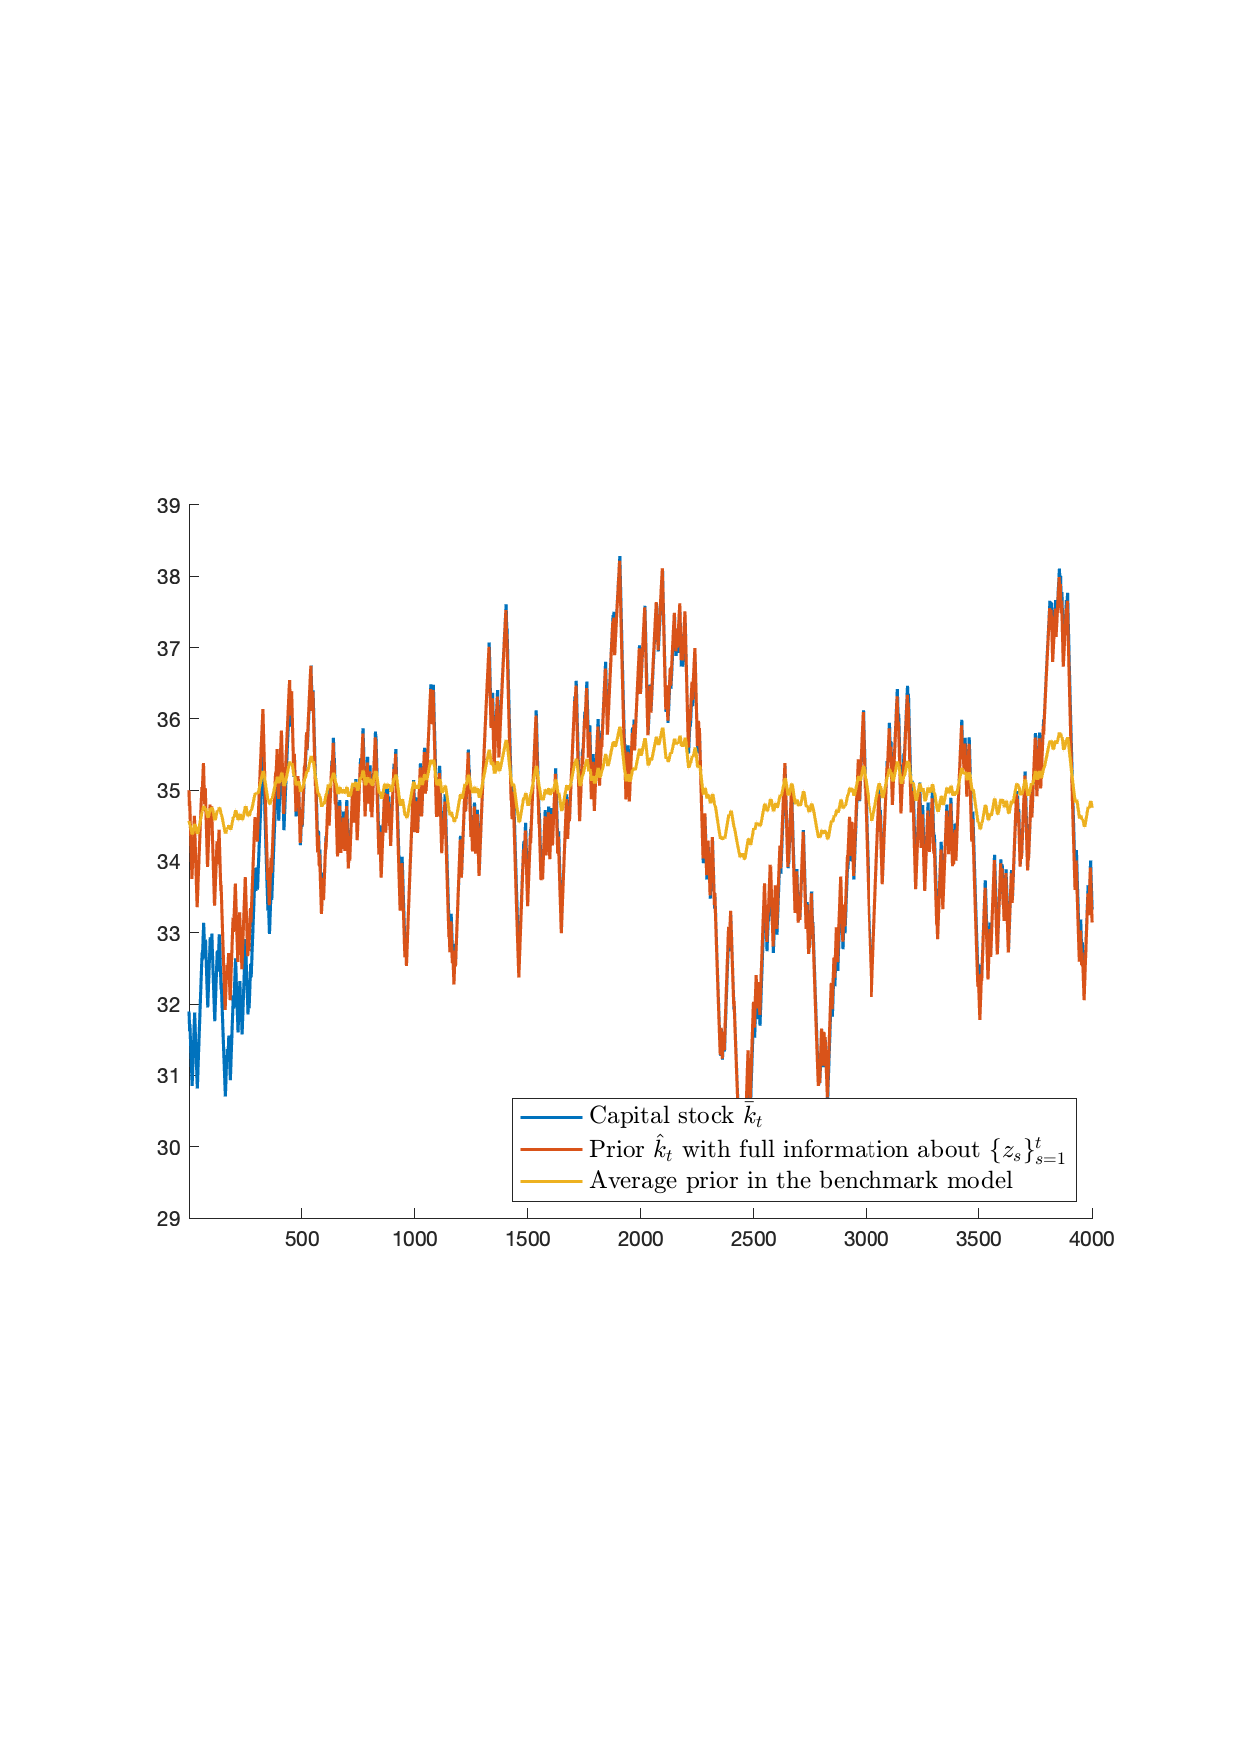
\includegraphics[viewport=-107bp 200bp 800bp 625bp,clip,scale=0.6]{_input/figure_b1}
\par\end{centering}
{\footnotesize\emph{Note}}{\footnotesize : Based on a simulation of
the calibrated benchmark model, the figure shows time series of the
mean (aggregate) capital stock $K_{t}=\bar{k}_{t}$ (blue line), the
prior expectation of current aggregate capital $\hat{K}_{t}=\hat{k}_{t}$
of households who acquire information about the current productivity
state every period (red line), and the average prior expectation in
the benchmark economy (yellow line). }{\footnotesize\par}
\end{figure}


\subsection{Extended Error-wealth Plot\label{app:model-fit-2}}

\begin{figure}[H]
\begin{centering}
\caption{Accuracy of Forecasts: Model vs. Data}
\label{fig-5-accuracy-u-2}\vspace{0.00cm}
\par\end{centering}
\begin{centering}
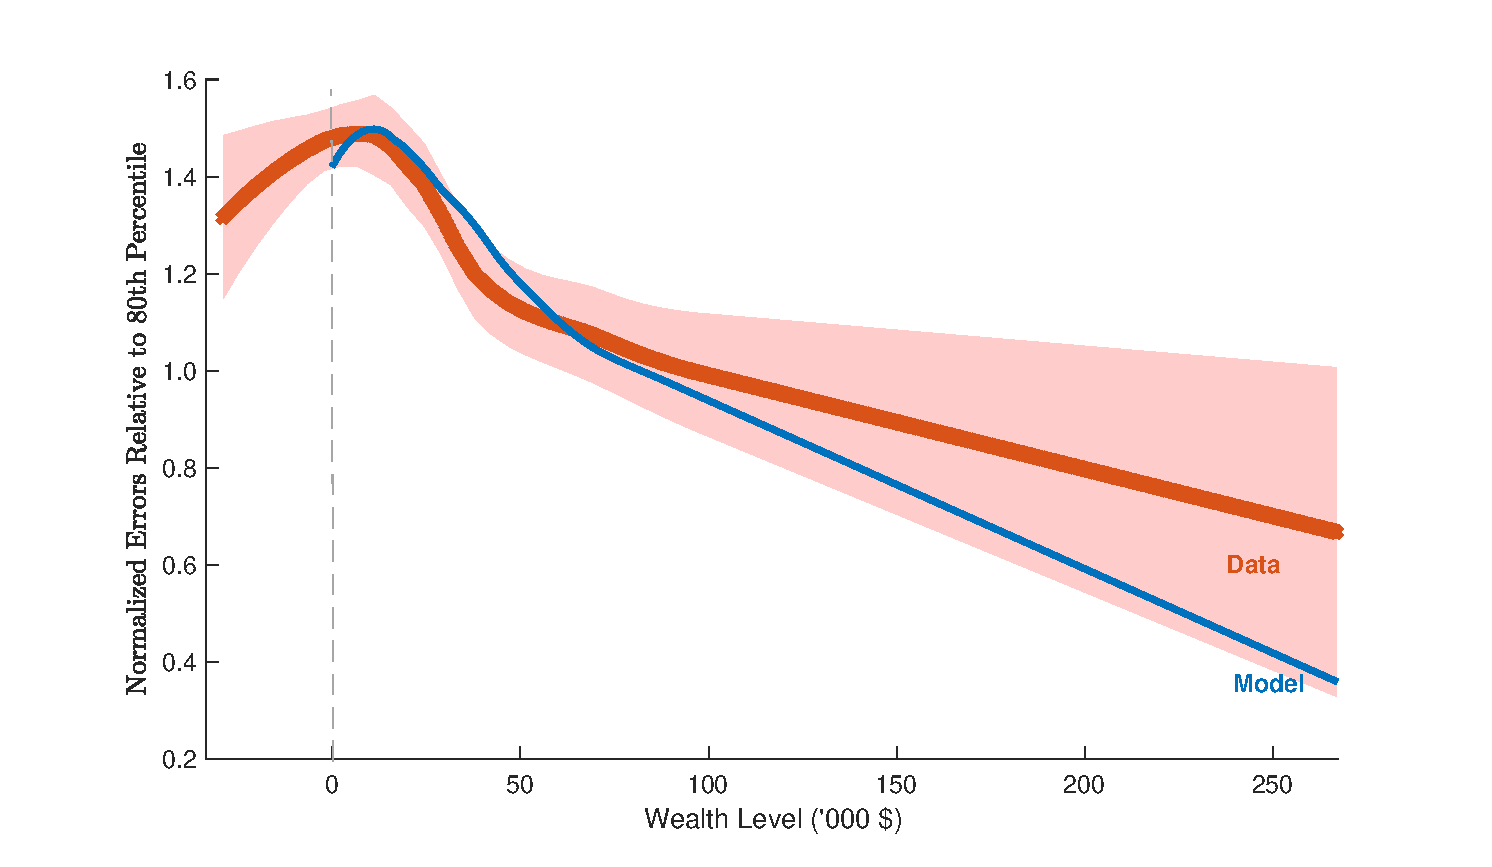
\includegraphics[viewport=-65bp 0bp 1000bp 400bp,clip,scale=0.58]{_input/figure_bii}
\par\end{centering}
{\footnotesize\emph{Note}}{\footnotesize : The figure shows the estimated
relationship between (the absolute value of) errors of the one-year
ahead probability of the unemployment rate increasing and household
wealth. We plot this relationship both in the SCE data and in the
calibrated model (see also Section \ref{sec:motivating-evidence}).
We use a local polynomial regression (the LOESS regression) to estimate
the non-linear relationship between the accuracy of household expectations
and household wealth. Error bands correspond to one-standard deviation
confidence bounds. We use 2020 values of quarterly U.S. household
income to convert values in the data and in the model to \$ (USD)
amounts.}{\footnotesize\par}
\end{figure}


\section{Extensions and Robustness}

\subsection{Mean-biased Capital Expectations\label{app-sub-sec:mean-bias}}

\begin{table}[H]
\caption{Mean-biased Capital Expectations\textemdash \% Relative to Full Information}

\label{app-tab:mean-biased-capital}

\textcolor{black}{\vspace{+0.39cm}}

\vspace{-0.22cm}
\begin{centering}
\textcolor{black}{\begin{tabular}{lccccc}
\toprule
\toprule
&\multicolumn{5}{c}{Panel (a): Business Cycle Moments}\\
& $\sigma(K)$ & $\sigma(Y)$ & $\sigma(I)$ & $\sigma(C)$ & $\text{Cor}(C,Y)$\\
\midrule
Endog. Info (P(learn K) = 1.0)) & 5.14 & 0.96 & 5.84 & -0.89 & -15.29 \\
[1em] Endog. Info (P(learn K) = 0.1)) & 11.07 & 1.80 & 7.86 & -1.49 & -18.06 \\
[1em] Benchmark Model & 64.28 & 11.04 & 13.63 & 5.11 & -3.07 \\
\midrule
& \multicolumn{5}{c}{}\\
&\multicolumn{5}{c}{Panel (b): Inequality Moments}\\
& $\text{Gini}(G)$ & $90/10$ & $99/1$ & $90/50$ & $\text{Cor}(K,Y)$\\
\midrule
Endog. Info (P(learn K) = 1.0)) & -0.40 & 1.36 & -1.30 & -0.14 & 2.93 \\
[1em] Endog. Info (P(learn K) = 0.1)) & -0.33 & 1.47 & -1.55 & 0.02 & 5.01 \\
[1em] Benchmark Model & 1.72 & 2.74 & 5.35 & 3.75 & 24.67 \\
\bottomrule
\bottomrule
\end{tabular}
}
\par\end{centering}
\vspace{0.22cm}

{\footnotesize\emph{Note}}{\footnotesize : The table shows model moments
in the calibrated model (``Benchmark Model''), as well as in models
in which households exogenously obtain information about the level
of the aggregate capital stock with a fixed probability $p\in[0,1]$
(``Endogenous Information (P(learn K)=$p$)''). The table reports
the percentage difference relative to the full-information version
for the same moments as those computed in Table \ref{tab:business-cycle-moments}
and Table \ref{tab:inequality-moments}.}{\footnotesize\par}
\end{table}


\subsection{Dynamics of the Wealth Distribution\label{subsec:inequality-dynamics}}

Section \ref{subsec:Distributional-Implications} studied the \emph{average}
\emph{consequences} of heterogeneous information for inequality. Table
\ref{tab:wealth-inequality-moments-dynamic} identifies the forces
that also make inequality volatile over time. It does so by comparing
the dynamics of different parts of the wealth distribution in the
benchmark economy to its full- and exogenous-information counterparts.
The main feature that stands out are the substantially larger swings
that occur in the benchmark economy. Relative to the case with full
information, the standard deviations of both the Gini coefficient
and, for example, the 99/50 percentile ratio are about 4\textendash 4.5
times higher in the benchmark economy\textemdash with inequality moments
that are, further, substantially larger than in the exogenous-information
case. 
\begin{table}
\caption{Dynamics of the Wealth Distribution}

\label{tab:wealth-inequality-moments-dynamic}\textcolor{black}{\vspace{-0.22cm}}

\textcolor{black}{\def\sym#1{\ifmmode^{#1}\else\(^{#1}\)\fi}

\begin{tabular*}{1.00\textwidth}{{l C{1.70cm} C{1.70cm} C{1.70cm} C{2.50cm} C{2.50cm}}}
\hline\hline\\[-1.8ex]
& $\sigma(\text{Gini})$ & $\sigma(\text{90/50})$ &  $\sigma(\text{99/50})$ & $\text{Cor}(\text{90th,} \text{10th})$ & $\text{Cor}(\text{99th,} \text{10th})$ \\ 
\hline 
Benchmark Model & 0.04 & 0.63 & 2.69 & 0.24 & -0.24\\ 
[1em] Exogenous Information & 0.03 & 0.42 & 1.92 & 0.40 & -0.20\\ 
[1em] Full  Information & 0.01 & 0.15 & 0.57 & 0.72 & 0.26\\ 
\hline
\hline
\end{tabular*}}

\vspace{0.22cm}

{\footnotesize\emph{Note}}{\footnotesize : Based on a long simulation
of the benchmark economy and the versions with exogenous and full
information, the table shows the standard deviations ($\sigma$) over
time of the Gini, the 90/50, and the 99/50 percentile ratios of the
wealth distribution ($k$), as well as the correlations ($\text{Cor})$
of, respectively, the 90th and 99th percentiles with the 10th percentile
of the wealth distribution.}{\footnotesize\par}
\end{table}

The key to understanding this increase in the volatility of wealth
dispersion lies, once more, in the impact that incomplete information
has on savings choices across the wealth distribution. With full information,
low-to-medium wealth households save less in booms, making their wealth
accumulation \emph{countercyclical}. The rich, by contrast, save more
when capital is high and returns low, but their overall wealth accumulation
remains \emph{countercyclical}\textemdash driven by countercyclical
returns to their stock of wealth. Taken together, the two imply that
the whole wealth distribution moves up and down in tandem, limiting
variations in inequality. 

The presence of incomplete information, by contrast, makes savings,
and thus wealth, at the bottom of the distribution \emph{more procyclical
(i.e. less} countercyclical\emph{)}, while\emph{ increasing} the countercyclicality
at the top of the wealth distribution. Both arise due to an increase
in savings errors that households make due to the presence of incomplete
information. Combined, the two explain the increased volatility of
inequality measures in Table \ref{tab:wealth-inequality-moments-dynamic}.
Finally, notice that\textemdash relative to the economies with \emph{exogenous
information}\textemdash the endogeneity of information in our benchmark
economy dampens the cyclicality of savings by medium-wealth households
(who have less-than-average information and own the bulk of the capital
stock) further. This, in turn, causes the volatility of wealth inequality
to be larger in our benchmark economy than in its exogenous-information
counterpart.\footnote{Because unemployment is countercyclical, individual earnings volatility
is generally higher in busts than in booms. As we mention above, this
increases the value of information for unemployed households, causing
their information acquisitions to be weakly countercyclical\textemdash more
information is bought by unemployed households in a bust. Overall,
however, information purchases are weakly procyclical, driven by the
behavior of the employed. This modulates the above discussed effects.}

\subsection{Decomposition of Changes in the Wealth Distribution\label{app-sub-sec:wealth-decomp}}

In this Appendix, we decompose the overall change in the wealth distribution
into three separate forces: (i) the change in the equilibrium law
of motion for capital; (ii) the presence of incomplete information;
and (iii) the heterogeneity that exists in information choices. Figure
\ref{fig-7-dist-composition} provides a breakdown of the overall
change into these three components.

\paragraph*{1. General Equilibrium:}

To isolate the general-equilibrium component, we conduct the following
experiment: We solve for household policy functions in the full-information
economy taking the benchmark economy\emph{'s} law of motion for capital,
$\tilde{H}(z,K)$, as given. We then simulate the economy with the
same sequence of shocks as in the full-information case and compare
the two wealth distributions. This experiment isolates the channel
by which the weakening of the mean-reversion of capital affects the
wealth distribution.\footnote{To be clear, households still optimize in this experiment and markets
clear in every period. Household expectations are simply inconsistent
with the true aggregate dynamics.}

Panel (b) in Figure \ref{fig-7-dist-composition} shows that the change
in the \emph{equilibrium law of motion for capital} in-and-of itself
\emph{dampens inequality}. All else equal, the weaker mean-reversion
in the benchmark economy causes a substantially more persistent law
of motion for capital, and thus increases the persistence of wages
and the rate of return on capital. This, in turn, causes stronger
income effects on savings, all else equal. Relative to the full-information
economy with its own  law of motion, a stronger correlation between
returns and savings at the bottom\textemdash and a lower correlation
at the top\textemdash of the distribution thus arises, reducing wealth
inequality. Recall that income effects reduce savings for low-to-medium
wealth households when the capital stock (and hence wages) are high,
while the opposite is the case for wealthy households as returns (and
hence financial income) decline with capital.\footnote{This mechanism is further amplified by the widening of the difference
between the income of employed and unemployed. The cross-sectional
dispersion of labor-market income increases with the volatility of
wages, and hence with the volatility of the capital stock. In equilibrium,
the difference between wages and unemployment benefits equal $(1-\mu)w_{t}=(1-\mu)(1-\alpha)z_{t}K_{t}^{\alpha}\bar{l}^{-\alpha}$,
whose average is increasing in the volatility of the capital stock
$K_{t}$. This, in turn, causes pre-cautionary savings to also increase,
especially near the bottom of the distribution, further reducing inequality.} General-equilibrium dynamics\textemdash through these mechanisms\textemdash partially
offset the widening of the wealth distribution.
\begin{figure}
\begin{centering}
\caption{Decomposition of Changes to the Wealth Distribution}
\label{fig-7-dist-composition}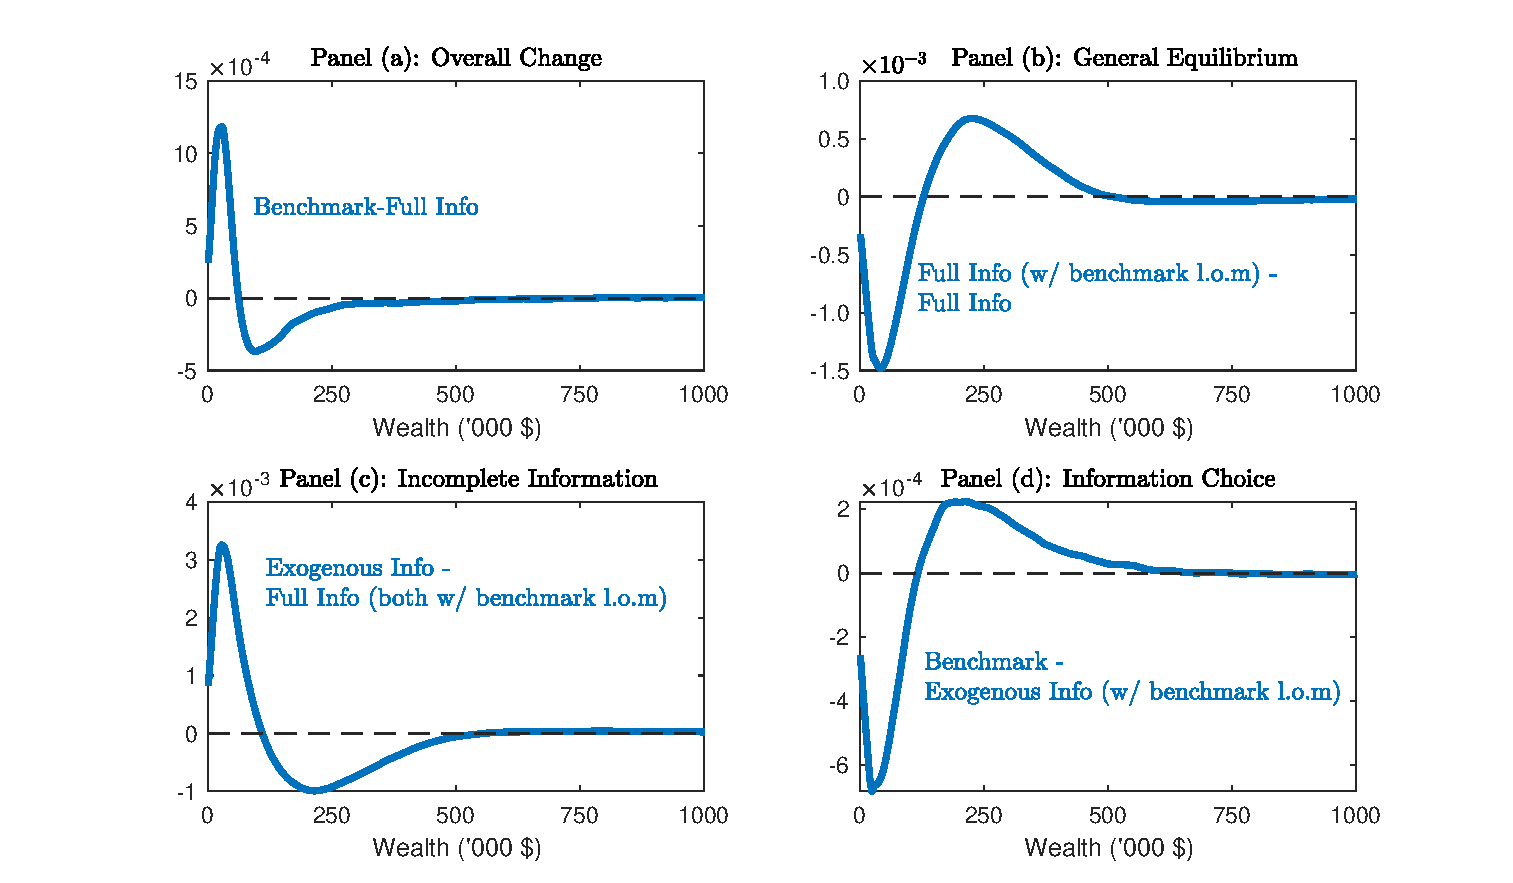
\includegraphics[viewport=56bp 0bp 945bp 420bp,scale=0.78]{_input/figure_c1}
\par\end{centering}
{\footnotesize\emph{Note}}{\footnotesize : The figure decomposes the
change in the average wealth distribution relative to the full-information
version of the benchmark economy (Panel (a)). Panel (b) shows the
difference in the average probability density function of the wealth
distribution between the full-information economy and the full-information
economy in which the law of motion for the capital stock equals that
in our benchmark economy. Panel (c) shows the difference between the
exogenous-information economy and the full-information economy, where
we equip both economies with a law of motion for the capital stock
equal to that in our benchmark economy. Finally, Panel (d) shows the
differences between our benchmark (endogenous-information) economy
and exogenous-information economy equipped with the law of motion
from our benchmark economy. The horizontal axis in all panels is household
wealth (capital levels) in '000 USD (\$). We use 2020 values of U.S.
household income to convert values in the model to \$ amounts. Probability
density functions are estimated from a simulated panel of household
capital holdings, using a kernel density estimator with the Epanechnikov
kernel.}{\footnotesize\par}
\end{figure}


\paragraph*{2. Incomplete Information:}

Our next experiment isolates the consequences that the\emph{ incompleteness}
\emph{of information} itself has on the wealth distribution. We solve
for the policy functions and simulate the distribution when households
have exogenously incomplete information but believe the law of motion
for capital is the one from the benchmark economy. By comparing the
distribution under this experiment to the previous one (full-information
with benchmark law of motion), we can quantify the effects of household
incomplete information on inequality. Panel (c) in Figure \ref{fig-7-dist-composition}
plots the difference between the two distributions.

The presence of incomplete information \emph{per se} explains the
lion's share of the widening of the wealth distribution. The dampened
correlation between savings and returns\textemdash caused by the incompleteness
of information\textemdash implies a widening of the wealth distribution
that is qualitatively similar but stronger than that in our benchmark
economy (Panel (a)). 

For low-to-medium wealth households, the presence of incomplete information
weakens the positive correlation that exists between returns and savings
in response to fluctuations in capital (Figure \ref{fig:4-savings-choices}).
This, in turn, reduces their average wealth accumulation. In effect,
these households make more ``mistakes'' with their savings choices\textemdash as
they are unable to effectively exploit periods of high returns on
capital\textemdash and end up poorer, as a result. 

The increased randomness by which households make savings choices,
by contrast, increases the share of wealthy households. These households'
informed savings policies, as mentioned in the main text, correlate
negatively with fluctuations in the return on capital (Figure \ref{fig:4-savings-choices}).
The presence of incomplete information thus increases the average
correlation between their savings and returns, increasing the average
wealth of high-wealth households. 

In essence, high-wealth households in our model\textemdash who also
feature close to linear policy functions, as they are far away from
the borrowing constraint\textemdash are akin to the households described
in \citet{piketty2003income}: The authors show that the combination
of exogenous random savings rates and linear policy functions can
generate Pareto tails in the wealth distribution. In our case, however,
the presence of incomplete information provides a microfoundation
for this type of ``random savings behavior'', as opposed to other
models that either assume exogenously stochastic savings rates or
random returns on savings.\footnote{That said, because the magnitude of the errors are comparatively small
relative to what is needed, in the benchmark model this force is not
sufficiently potent to generate a thick Pareto tail of wealth (cf.
Section \ref{subsec:Matching-the-Wealth}).}

\paragraph*{3. Information Choice:}

Our final decomposition compares the distribution from the previous
experiment (exogenous, incomplete information with benchmark law of
motion) with the benchmark distribution. This difference isolates
the effects that \emph{heterogeneous} \emph{information choices} have
on the wealth distribution. We plot differences in Panel (d) in Figure
\ref{fig-7-dist-composition}.

All else equal, the more informed households in our benchmark economy
are the poor, unemployed households and the rich households with substantial
amounts of wealth (Figure \ref{fig-3-information-prob}). These households,
who are better informed than their exogenous-information counterparts,
make fewer savings mistakes\textemdash they are, on average, better
able to exploit differences in rates of return on capital. As a result,
the existence of \emph{heterogeneous} \emph{information} causes fewer
wealth-poor (\$0-50,000) as well as wealth-rich (above \$750,000)
households. The decline in ``random savings'' caused by the presence
of additional information allows households near the bottom-end of
the wealth distribution to better correlate their savings with its
rate of return, allowing these households to better accumulate wealth.
By contrast, the decline in ``random savings'' of the wealthy drives
down their realized saving.

\paragraph*{Summary and Quantification:}

In sum, the presence of heterogeneous, incomplete information leads
to rich and complex changes in the wealth distribution. On the one
hand, the presence of incomplete information widens the wealth distribution
by leading to ``random savings behavior''. On the other hand, the
existence of heterogeneity in information choices, all else equal,
dampens this increase  by allowing the more exposed households\textemdash the
poor and the wealthy\textemdash to acquire information to make better
savings choices. This dampening effect is then further amplified by
the weakening of the mean-reversion of capital further lessening any
increase in inequality.\footnote{Notice that while heterogeneity in information acquisition by itself
decreases inequality, our benchmark economy features more inequality
than its exogenous information counterpart (Table \ref{tab:inequality-moments}).
This is due to the weaker general equilibrium dynamics in our benchmark
model with heterogeneous information.} On balance, we find that the former effect dominates, leading to
a modest overall increase in inequality (Table \ref{tab:inequality-moments}).
Table \ref{app-tab:wealth-dist-decomposition} decomposes the overall
increase in different summary measures of inequality (e.g., the Gini)
and shows that the \emph{modest net increase} in inequality is comprised
of \emph{large, offsetting gross effects}. The 2 percent increase
in the Gini is, for example, comprised of an 8 percent increase due
to incomplete information counteracted by 4 and 2 percent decreases,
respectively, due to general equilibrium dynamics and heterogeneity
in information choices. The combined effects of heterogeneous information
are subtle\textemdash and, crucially, affect different parts of the
distribution differentially.

\begin{table}[H]
\caption{Decomposition of Wealth Distribution Changes\textemdash \% Relative
to Full Information}

\label{app-tab:wealth-dist-decomposition}

\vspace{-0.01cm}
\begin{centering}
\textcolor{black}{\def\sym#1{\ifmmode^{#1}\else\(^{#1}\)\fi}

\begin{tabular*}{0.90\textwidth}{{l C{2.00cm} | C{2.00cm} C{2.00cm} C{2.25cm} C{2.00cm}}}
\hline\hline\\[-1.8ex]
&  Overall & GE  & Incomplete Info.  & Heterogenous Info. & Interaction\\
\cline{2-6} \\[-1.8ex]
Gini Statistic              &1.62  & -3.92  & 7.54  & -1.65	  &  -0.35 \\ 
[1em] $90/10-$ratio   & 2.72 & -2.91	& 7.31  & -1.40   &  -0.27 \\ 
[1em] $99/1-$ratio    & 5.04 &-13.90	& 20.65 &	-3.73  &   2.03 \\ 
%Gini Statistic              & 1.50 & -4.04   & 7.54  & -1.65 & -0.35 \\ 
%[1em] $90/10-$ratio  & 2.64 & -2.99   & 7.31  & -1.40 & -0.28 \\ 
%[1em] $99/1-$ratio    & 4.67 & -13.92 & 20.67 & -3.73 & 1.65 \\ 
\hline
\hline
\end{tabular*}
}
\par\end{centering}
\vspace{0.22cm}

{\footnotesize\emph{Note}}{\footnotesize : This table decomposes the
overall change in the wealth distribution (relative to the full-information
case) into the forces highlighted in Section \ref{subsec:Distributional-Implications}.
We focus, for concreteness, on the Gini, the 90/10-ratio, and the
99/1-ratio. Similar results hold for other summary inequality measures.}{\footnotesize\par}
\end{table}


\subsection{Acyclical Income Taxes\label{app-sub-sec:acycl-taxes}}
\begin{center}
\enlargethispage{2\baselineskip}
\begin{table}[H]
\caption{Business Cycle Moments\textemdash Acyclical Income Taxes}

\label{tab:business-cycle-moments-acyc}\textcolor{black}{\vspace{-0.22cm}}

\textcolor{black}{\def\sym#1{\ifmmode^{#1}\else\(^{#1}\)\fi}

\begin{tabular*}{\textwidth}{l C{1.70cm} C{1.70cm} C{1.70cm} C{1.70cm} C{1.70cm} C{1.70cm} C{1.70cm}}
\hline\hline\\[-1.8ex]
& \multicolumn{6}{c}{Panel (a): Level of Moments}\\
& $\sigma(K)$ & $\sigma(Y)$ & $\sigma(I)$ & $\sigma(C)$ &$\text{Cor}(C,Y)$&$\text{Cor}(I,Y)$ \\
\cline{2-7} \\[-1.8ex]
Benchmark Model & 3.98 & 3.15 & 9.33 & 0.98 & 0.64 & 0.99\\ 
[1em] Exogenous Information & 3.30 & 3.05 & 9.00 & 0.94 & 0.61 & 0.99\\ 
[1em] Full  Information & 2.39 & 2.93 & 8.14 & 0.94 & 0.69 & 0.98\\ 
\hline
&&&\\
& \multicolumn{6}{c}{Panel (b): Percent  Difference w.r.t. Full Information} \\ 
& $\sigma(K)$ & $\sigma(Y)$ & $\sigma(I)$ & $\sigma(C)$ & $\text{Cor}(C,Y)$ & $\text{Cor}(I,Y)$  \\
\cline{2-7}\\[-1.8ex]
Benchmark Model & 66.13 & 7.72 & 14.63 & 4.76 & -8.26 & 0.55\\ 
[1em] Exogenous Information & 37.92 & 4.13 & 10.55 & 0.01 & -11.85 & 0.30\\ 
\hline 
\hline
\end{tabular*}}

\vspace{0.22cm}

{\footnotesize\emph{Note}}{\footnotesize : This table shows the standard
deviation $\sigma$ of the logarithm of economy-wide capital ($K$),
output ($Y)$, investment ($I$), and consumption ($C)$. In addition,
the table shows the correlation between aggregate consumption, investment,
and output, respectively (e.g., $\text{Cor}(I,Y)$). The table depicts
these moments for the benchmark model (``Benchmark Model'') as well
as the two comparison models with full and exogenous information (``Full
Information'' and ``Exogenous Information'', respectively).}{\footnotesize\par}
\end{table}
\begin{table}[H]
\caption{Inequality Moments\textemdash Acyclical Income Taxes}

\label{tab:inequality-moments-acyc}\textcolor{black}{\vspace{-0.22cm}}

\begin{centering}
\begin{centering}
\textcolor{black}{\def\sym#1{\ifmmode^{#1}\else\(^{#1}\)\fi}
{\centering
\begin{tabular*}{\textwidth}{@{\extracolsep{\fill}} l c c c c c}
\hline\hline\\[-1.8ex]
& \multicolumn{5}{c}{Panel (a): Level of Moments}\\
 & Gini G& $90/10$ & $99/1$ & $90/50$  &$\text{Cor}(K,Y )$ \\
\cline{2-6} \\[-1.8ex]
Benchmark Model & 0.51 & 14.48 & 337.33 & 3.47 & 0.54\\ 
[1em] Exogenous Information & 0.51 & 14.45 & 331.79 & 3.42 & 0.49\\ 
[1em] Full  Information & 0.50 & 14.08 & 320.20 & 3.36 & 0.43\\ 
\hline
&&&\\
& \multicolumn{5}{c}{Panel (b): Percent  Difference w.r.t. Full Information} \\ 
 & Gini G& $90/10$ & $99/1$ & $90/50$  &$\text{Cor}(K,Y )$  \\
\cline{2-6} \\[-1.8ex]
Benchmark Model & 1.86 & 2.84 & 5.35 & 3.38 & 25.11\\ 
[1em] Exogenous Information & 1.28 & 2.63 & 3.62 & 1.77 & 14.41\\ 
\hline
\hline
\end{tabular*}\par}}
\par\end{centering}
\end{centering}

\vspace{0.22cm}

{\footnotesize\emph{Note}}{\footnotesize : The table shows the Gini
coefficient of the capital distribution ($G)$, as well as the 90/10,
99/1, and 90/50 percentile ratios of the wealth distribution. In addition,
the table shows the correlation between the logarithm of capital and
log. output ($Y)$ ($Cor(K,Y)$). The table depicts these moments
for the benchmark model (``Benchmark Model'') as well as the two
comparison models.}{\footnotesize\par}
\end{table}
\par\end{center}

%\thispagestyle{empty} 

\subsection{Costs of Information and Alternative Models\label{app-subsec-resource-cost-information}}

\vspace{-0.38cm}\enlargethispage{4\baselineskip}
\begin{table}[H]
\caption{Business Cycle Moments\textemdash No Costs of Information}

\label{tab:business-cycle-moments-angelvsdemon}\textcolor{black}{\vspace{-0.38cm}}

\begin{centering}

\textcolor{black}{\def\sym#1{\ifmmode^{#1}\else\(^{#1}\)\fi}

\begin{tabular*}{0.9\textwidth}{l  C{1.70cm} C{1.70cm} C{1.70cm} C{1.70cm} C{1.70cm}}
\hline\hline\\[-1.8ex]
& $\sigma(K)$ & $\sigma(Y)$ & $\sigma(I)$ & $\sigma(C)$ & $\text{Cor}(C,Y)$ \\ 
\hline 
Benchmark Model & 5.05 & 3.38 & 11.98 & 1.25 & 0.7   \\ 
 			     &        &         &           &         &           \\
		& \multicolumn{5}{c}{Panel (a): With Costs of Information}\\
		\hline
Exogenous Information & 4.19 & 3.22 & 11.56 & 1.19 & 0.67  \\ 
Full Information & 3.07 & 3.04 & 10.54 & 1.19 & 0.72    \\ 
 			     &        &         &           &         &           \\
		& \multicolumn{5}{c}{Panel (b): Without Costs of Information}\\
		\hline
Exogenous Information  & 4.19 & 3.22 & 11.55 & 1.19 & 0.67  \\ 
Full Information              & 3.07 & 3.04 & 10.54 & 1.19 & 0.72  \\ 
 			     &        &         &           &         &           \\
		& \multicolumn{5}{c}{Panel (c): Percentage Difference due to  Costs}\\
		\hline
Exogenous Information & -0.06 & -0.02 & -0.06 & -0.11 & -0.04\\ 
Full Information & -0.02 & -0.00 & 0.00 & -0.21 & -0.03\\ 
\hline 
\hline
\end{tabular*}}

\end{centering}

\vspace{0.38cm}

{\footnotesize\emph{Note}}{\footnotesize : The table shows the standard
deviation $\sigma$ of the logarithm of capital ($K$), output ($Y)$,
investment ($I$), and consumption ($C)$. In addition, the table
shows the correlation between consumption and output ($\text{Cor}(C,Y)$).
The table shows these moments for the benchmark model (``Benchmark
Model''), the two comparison models with full and exogenously limited
information (``Full Information'' and ``Exogenous Information'',
respectively), as well as versions of the comparison models in which
all costs of information are set equal to zero.}{\footnotesize\par}
\end{table}
\vspace{-0.46cm}
\begin{table}[H]
\caption{Inequality Moments\textemdash No Costs of Information}

\label{tab:inequality-moments-angelvsdemon}\textcolor{black}{\vspace{-0.38cm}}

\begin{centering}

\textcolor{black}{\def\sym#1{\ifmmode^{#1}\else\(^{#1}\)\fi}


\begin{tabular*}{0.92\textwidth}{l  C{1.70cm} C{1.70cm} C{1.70cm} C{1.70cm} C{1.90cm}}
\hline\hline\\[-1.8ex]
	& $\text{Gini}(K)$ & $90/10$ & $99/1$  & $90/50$ &  $\text{Cor}(K, Y)$  \\ 
\hline 
Benchmark Model & 0.51 & 14.53 & 345.3 &  3.51  & 0.62  \\ 
 			     &        &         &           &         &           \\
		& \multicolumn{5}{c}{Panel (a): With Costs of Information}\\
		\hline
Exogenous Information & 0.51 & 14.51 & 339.3 & 3.45 & 0.56  \\ 
Full Information & 0.50 & 14.15 & 327.8 & 3.39  &0.49 \\ 
			     &        &         &           &         &           \\
		& \multicolumn{5}{c}{Panel (b): Without Costs of Information}\\
		\hline
Exogenous Information & 0.51 & 14.48 & 336.6 & 3.43 & 0.56\\ 
Full Information & 0.50 & 14.12 & 325.1 & 3.37 & 0.49\\ 
			     &        &         &           &         &           \\
		& \multicolumn{5}{c}{Panel (c): Percentage Difference due to  Costs}\\
		\hline
Exogenous Information & -0.28 & -0.19 & -0.78 & -0.36 & -0.03\\ 
Full Information             & -0.28 & -0.17 & -0.81 & -0.36 & -0.01\\ 
\hline 
\end{tabular*}}

\end{centering}

\vspace{0.38cm}

{\footnotesize\emph{Note}}{\footnotesize : The table shows the Gini
coefficient of the capital distribution ($\text{Gini})$, as well
as the 90/10, 99/1, and 90/50 percentile ratios of the capital distribution.
In addition, the table shows the correlation between the logarithm
of capital and log. output ($Y)$ ($\text{Corr}(K,Y)$). The table
shows these moments for the benchmark model (``Benchmark Model''),
the two comparison models, as well as versions of the comparison models
in which all costs of information are set equal to zero.}{\footnotesize\par}
\end{table}
%\thispagestyle{empty} 

\subsection{Homotheticity of Information Costs \label{app-subsec-c2-1}}

\begin{figure}[H]
\caption{Accuracy Across the Wealth Distribution\textemdash Scaled Utility
Cost}
\label{fig:app-unemployment-errors-scaled-ucost}
\begin{centering}
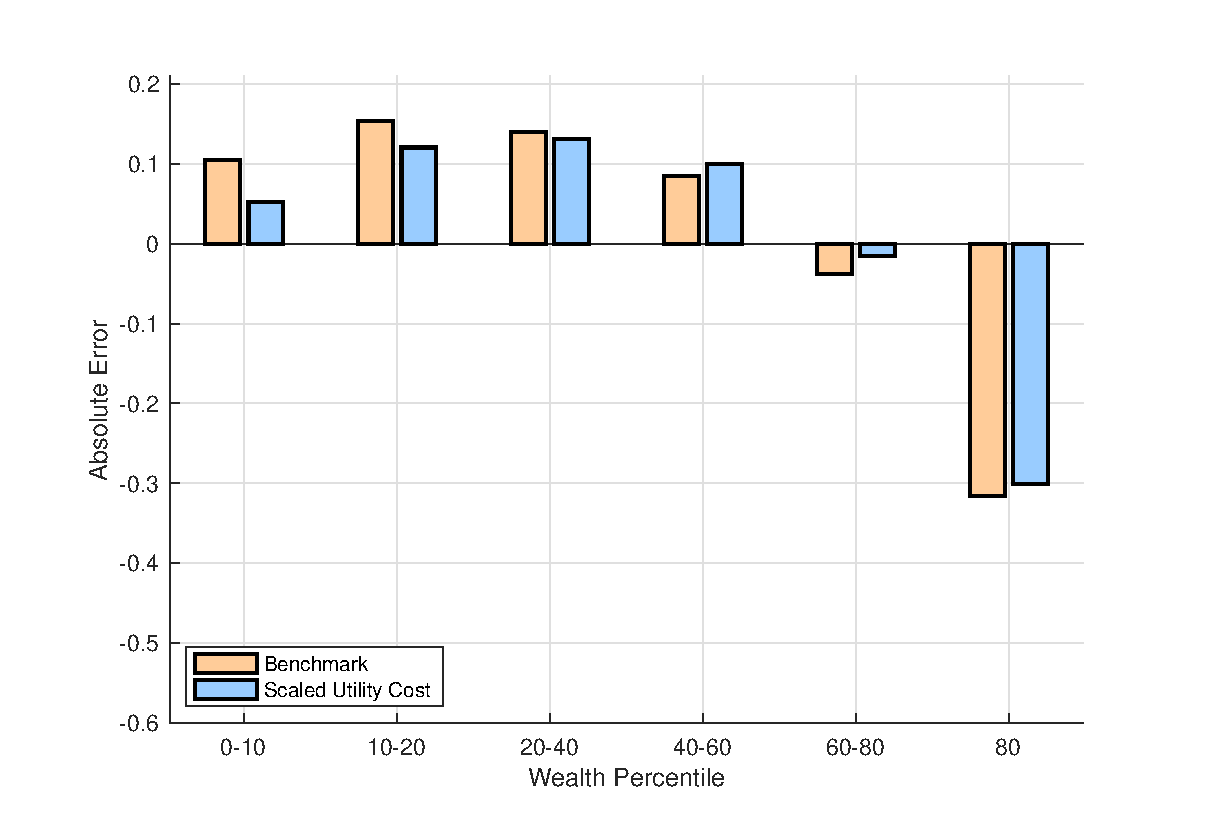
\includegraphics[scale=0.74]{_input/figure_c2}
\par\end{centering}
\hspace{-0.65cm}

{\footnotesize\emph{Note}}{\footnotesize : The figure plots the difference
between the average one-year-ahead accuracy of unemployment forecasts
within wealth deciles/quintiles and the overall average taken across
all wealth levels. Accuracy is measured by the absolute value of unemployment
errors (Appendix \ref{app:data}). We plot these accuracies both for
the calibrated benchmark model and for the calibrated model with the
scaled utility cost.}{\footnotesize\par}
\end{figure}
\vspace{-0.48cm}
\begin{table}[H]
\caption{Model Moments\textemdash Scaled Utility Cost}

\textcolor{black}{\label{app-tab:monetary-cost-endo-1}\vspace{-0.22cm}}

\begin{centering}

\textcolor{black}{\begin{tabular}{lccccc}
\toprule
\toprule
&\multicolumn{5}{c}{Panel (a): Business Cycle Moments}\\
& $\sigma(K)$ & $\sigma(Y)$ & $\sigma(I)$ & $\sigma(C)$ & $\text{Cor}(C,Y)$\\
\midrule
Benchmark & 5.05 & 3.38 & 11.98 & 1.25 & 0.70\\ 
Scaled Utility Cost & 4.96 & 3.36 & 11.92 & 1.24 & 0.70\\ 
Difference \% & -1.77 & -0.52 & -0.43 & -0.67 & -0.37\\ 
\midrule
&\multicolumn{5}{c}{Panel (b): Inequality Moments}\\
& $\text{Gini}(K)$ & $90/10$ & $99/1$ & $90/50$ & $\text{Cor}(K,Y)$ \\
\midrule
Benchmark & 0.51 & 14.53 & 345.3 &3.51 & 0.62 \\ 
Scaled Utility Cost & 0.51 & 14.49 & 343.1 & 3.50 & 0.61 \\ 
Difference \% & -0.19 & -0.33 & -0.64 & -0.51 & -0.85 \\ 
\bottomrule
\bottomrule
\end{tabular}
}

\end{centering}

\vspace{0.22cm}

{\footnotesize\emph{Note}}{\footnotesize : The table shows the same
model moments as in Section \ref{sec:quantitative-results} for the
benchmark (endogenous information) model (``Benchmark'') with and
without the scaled utility cost of information $\kappa$ set equal
to zero.}{\footnotesize\par}
\end{table}
\pagebreak

\begin{figure}[H]
\caption{Accuracy Across the Wealth Distribution\textemdash No Resource Cost}
\label{fig:app-unemployment-errors-mon-cost}
\begin{centering}
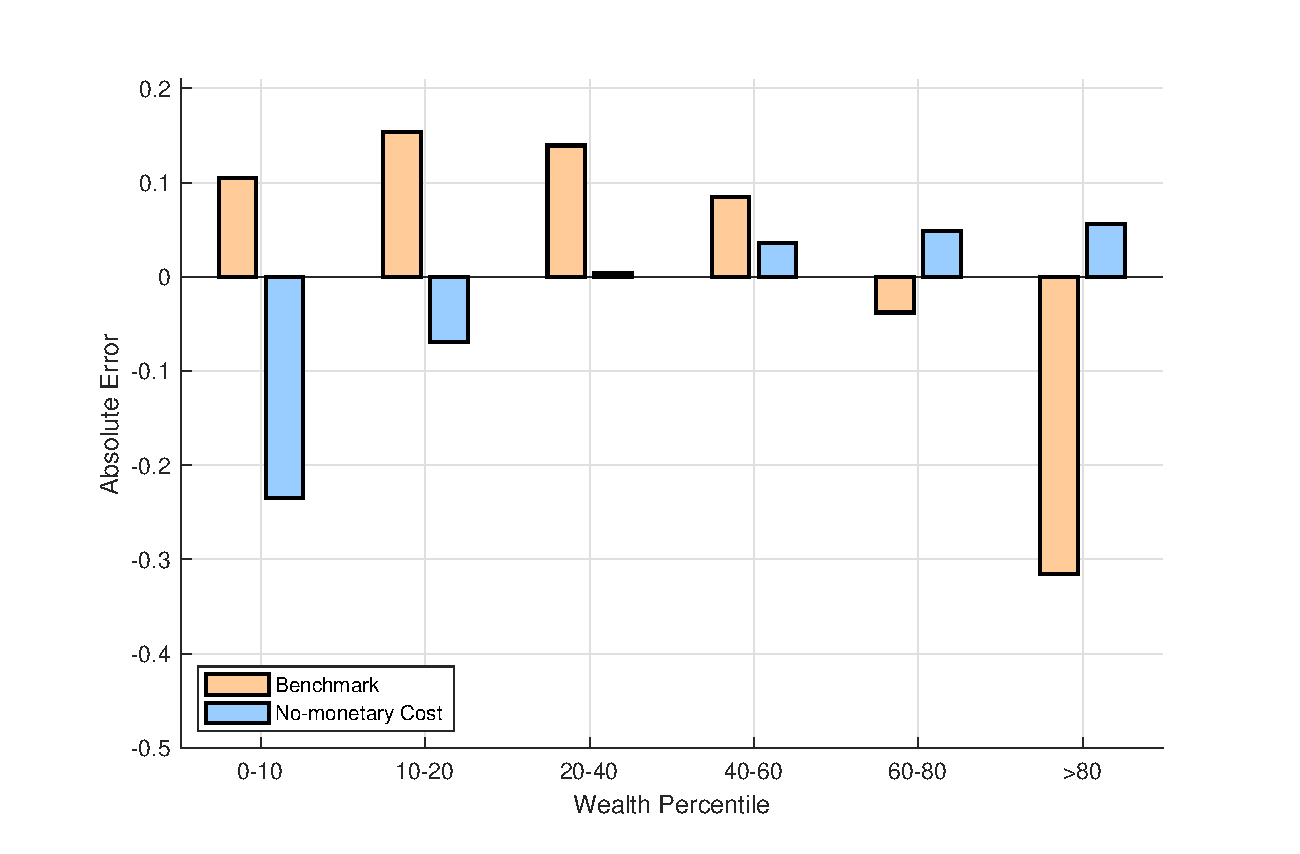
\includegraphics[scale=0.74]{_input/figure_c3}
\par\end{centering}
\hspace{-0.65cm}

{\footnotesize\emph{Note}}{\footnotesize : The figure plots the difference
between the average one-year-ahead accuracy of unemployment forecasts
within wealth deciles/quintiles and the overall average taken across
all wealth levels. Accuracy is measured by the absolute value of unemployment
errors (Appendix \ref{app:data}). We plot these accuracies both for
the calibrated benchmark model and for the calibrated model with no
resource cost.}{\footnotesize\par}
\end{figure}

\begin{table}[H]
\caption{Model Moments\textemdash No Resource Costs}

\textcolor{black}{\label{app-tab:monetary-cost-endo}\vspace{-0.22cm}}

\begin{centering}

\textcolor{black}{\def\sym#1{\ifmmode^{#1}\else\(^{#1}\)\fi}

\begin{tabular*}{0.92\textwidth}{l  C{1.70cm} C{1.70cm} C{1.70cm} C{1.70cm} C{1.90cm}}
\hline\hline\\[-1.8ex]
			& \multicolumn{5}{c}{Panel (a): Business Cycle Moments}\\
	& $\sigma(K)$ & $\sigma(Y)$ & $\sigma(I)$ & $\sigma(C)$ & $\text{Cor}(C,Y)$ \\ 
\hline 
With Resource Cost     & 5.05 & 3.38 & 11.98 & 1.25 & 0.70  \\  
Without Resource Cost & 4.11 & 3.20 & 11.48 & 1.19 & 0.68\\ 
\hline 
 Difference \%               &-18.49 & -5.10 & -4.11 & -5.01 & -3.82\\ 
\hline 
		     &        &         &           &         &           \\
		& \multicolumn{5}{c}{Panel (b): Inequality Moments}\\
		& $\text{Gini}(K)$  & $90/10$ & $99/1$ & $90/50$ & $\text{Cor}(K, Y )$  \\ 
\hline
With Resource Cost & 0.51 & 14.53 & 345.30 & 3.51 & 0.62\\ 
Without Resource Cost & 0.50 & 14.12 & 328.16 & 3.39 & 0.56\\ 
\hline 
 Difference \%               & -1.48 & -2.86 & -4.96 & -3.50 & -9.08\\ 
\hline
\hline
\end{tabular*}}

\end{centering}

\vspace{0.22cm}

{\footnotesize\emph{Note}}{\footnotesize : The table shows the same
model moments as in Section \ref{sec:quantitative-results} for the
benchmark (endogenous information) model (``Benchmark Model'') with
and without the resource cost of information $\eta$ set equal to
zero.}{\footnotesize\par}
\end{table}

\newpage

\subsection{Matching the Wealth Distribution\label{app-subsec-wealthy}}

\subsubsection{Extended Model Framework}

A representative final-goods producer bundles varieties $j\in\mathcal{J}$
in accordance with: 
\begin{equation}
Y_{t}=\left(\int y_{jt}^{\frac{\omega-1}{\omega}}d_{j}\right)^{\frac{\omega}{\omega-1}}\label{app-eq:dixit-stiglitz}
\end{equation}
with elasticity of substitution $\omega>1$. Each of the differentiated
goods is sold at price $p_{j}>0$, so that the ideal price level equals
$P_{t}=\left(\int p_{jt}^{1-\omega}dj\right)^{\frac{1}{1-\omega}}$,
which we normalize to one. Consistent with this structure, the demand
for each variety is
\[
y_{jt}=p_{jt}^{-\omega}Y_{t}.
\]
Intermediate goods firms produce using the production technology in
(\ref{eq:technology}) and are characterized by the same assumptions
as firms in our benchmark framework.

There are two types of households: A mass $m\in(0,1)$ of worker-households
and a mass $1-m$ of entrepreneur-households. Worker-households are
identical to households in our benchmark model. Entrepreneurs, by
contrast, receive all pure rents (i.e., profit income) in the economy
but no labor income. Entrepreneurs are across all other dimensions
identical to worker-households.\textcolor{pink}{{} }We assume the existence
of fixed transition probability matrix, $\Pi_{T}$, modeled as in
\citet{bayer2024shocks}, so that worker-households transition to
become entrepreneur-households, and vice versa. We allow for borrowing
and assume that $k_{i}^{\prime}\geq k_{\min}\in\mathbb{R}_{-}.$ All
debts are forgiven upon death. All other model details are as described
in Section \ref{sec:model}.

\subsubsection{Alternative Calibration and Quantification}

We follow a similar calibration strategy to that of our benchmark
model. To target the bottom of the wealth distribution, we set $k_{\text{min}}=-4$
and increase the replacement rate to 45 percent, in line with the
average value for the U.S. in 2022. This ensures that the 10th percentile
of the wealth distribution features $k_{i}=0$, on average, as in
the data. We set the additional parameters\textemdash the mass of
entrepreneurs and the CES elasticity\textemdash to $1$ percent and
so as to target the top 10 percent wealth share in the data, respectively,
consistent with \citet{bayer2024shocks}. We set the transition matrix,
$\Pi_{T}$, to the values estimated in \citet{guvenen2014risky},
in line with the approach in \citet{bayer2024shocks}. Finally, we
set resource cost of information and scale parameter for the utility
cost of information so as to once more target the mean and cross-sectional
standard deviation of forecasts errors in the SCE. We also recalibrate
the discount factor to target the same capital-to-output ratio as
before. Figure \ref{fig:app-1-unemployment-errors} compares the accuracy
of unemployment forecasts across the wealth distribution with that
in the benchmark model; Table \ref{app-tab:extended-model-moments}
shows the business-cycle and inequality moments. We note that because
of the possibility of negative wealth, certain percentile ratios of
the wealth distributions, such as the 90/10-ratio, are ill-defined,
which is why they are excluded from the table.\footnote{Indeed, the average value is, for example, $\infty$ for the 90/10-ratio,
as the 10th percentile of the wealth distribution occasionally hits
zero in the simulation per its calibration. }\textcolor{orange}{{} }

\begin{figure}[H]
\caption{Accuracy Across the Wealth Distribution\textemdash Extended and Benchmark
Model}
\label{fig:app-1-unemployment-errors}\vspace{-0.24cm}
\begin{centering}
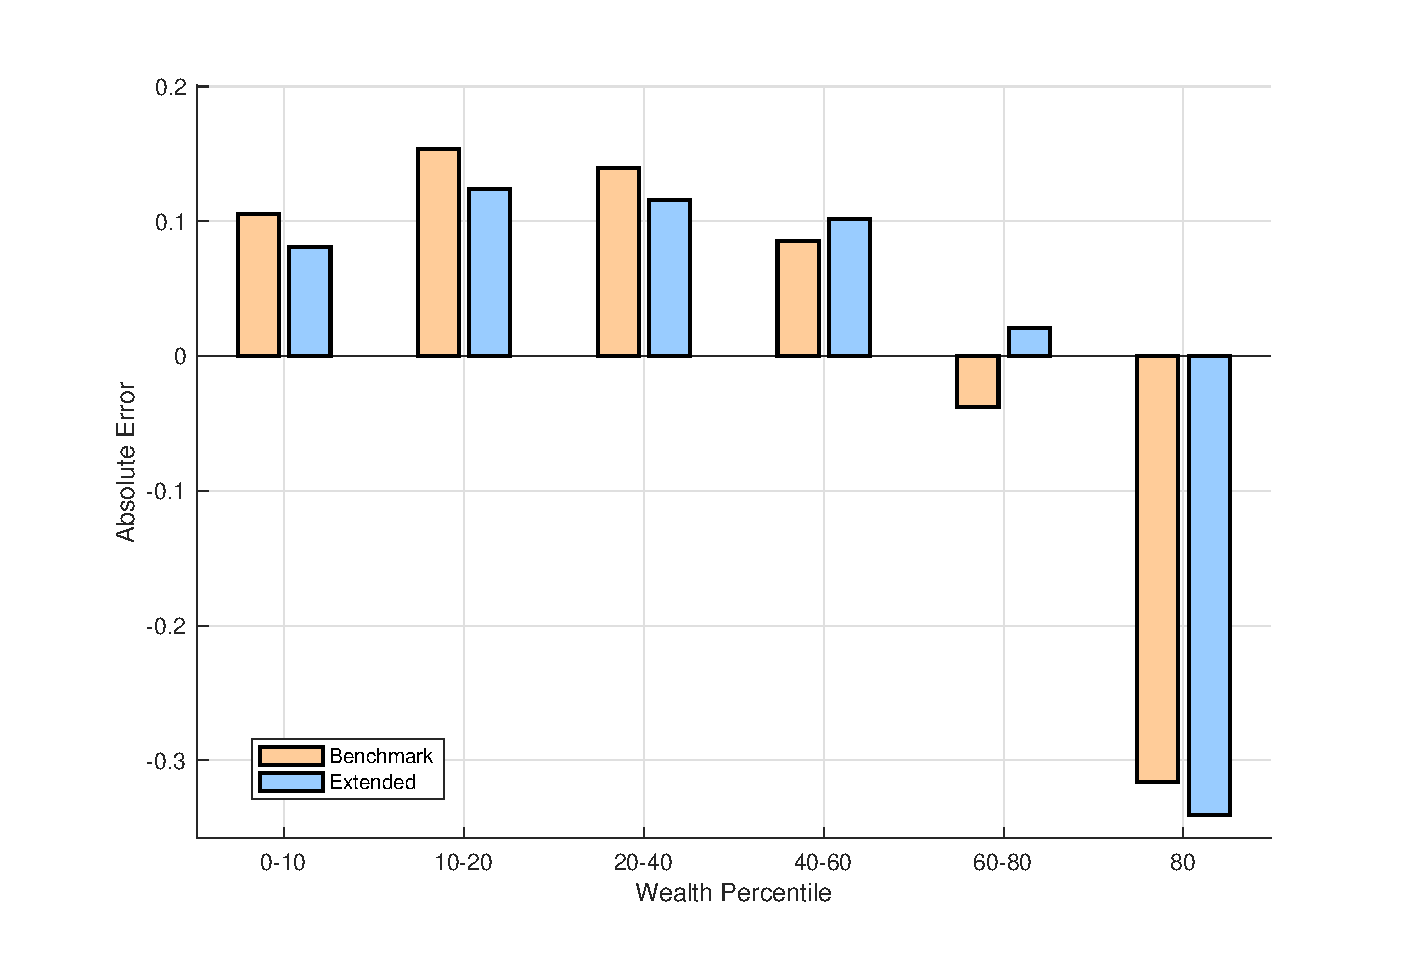
\includegraphics[scale=0.65]{_input/figure_c4}
\par\end{centering}
\vspace{-0.24cm}

{\footnotesize\emph{Note}}{\footnotesize : The figure plots the difference
between the average one-year ahead accuracy of unemployment forecasts
within wealth deciles/quintiles and the overall average taken across
all wealth levels. Accuracy is measured by the absolute value of unemployment
errors (Appendix \ref{app:data}). We plot these accuracies both for
the calibrated benchmark model and for the calibrated extended model
that matches the wealth distribution. }{\footnotesize\par}
\end{figure}

\begin{table}[H]
\caption{Extended Model Moments: Business Cycle and Inequality}

\textcolor{black}{\label{app-tab:extended-model-moments}\vspace{-0.22cm}}

\begin{centering}

\textcolor{black}{\def\sym#1{\ifmmode^{#1}\else\(^{#1}\)\fi}

\begin{tabular*}{0.98\textwidth}{l  C{1.70cm} C{1.70cm} C{1.70cm} C{1.70cm} C{1.90cm}}
\toprule\toprule\\[-1.8ex]

&\multicolumn{5}{c}{Panel (a): Business Cycle Moments}\\
& $\sigma(K)$ & $\sigma(Y)$ & $\sigma(I)$ & $\sigma(C)$ & $\text{Cor}(C,Y)$\\
\midrule
Endogenous Information (A)        & 4.69 & 3.22 & 14.40 & 1.20 & 0.64\\ 
Exogenous Information (B)           & 3.45 & 3.03 & 13.55 & 1.08 & 0.59\\ 
Full Information (C)                       & 2.74 & 2.95 & 12.14 & 1.14 & 0.71\\ 
Difference \%  (A vs C)                 & 71.00 & 8.99 & 18.57 & 5.29 & -9.72\\ 
\midrule
&&&&&\\
&\multicolumn{5}{c}{Panel (b): Inequality Moments}\\
& $\text{Gini}(K)$ &   & $90/50 $  &  & $\text{Cor}(K,Y)$ \\
\midrule
Endogenous Information (A)  & 0.76 & &10.37 & & 0.56     \\ 
Exogenous Information  (B)   & 0.73 & &  7.37 & & 0.47    \\  
Full Information (C)                & 0.70 & &  6.41& & 0.44    \\ 
Difference \%  (A vs C)          & 8.60 & & 61.76  & & 27.48 \\ 

\bottomrule
\bottomrule
\end{tabular*}


}

\end{centering}

\vspace{0.38cm}

{\footnotesize\emph{Note}}{\footnotesize : Panel (a) and (b) show the
same model moments as in Table \ref{tab:business-cycle-moments} and
\ref{tab:inequality-moments} but for the extended benchmark model
(endogenous information) as well as its full-information and exogenous-information
counterparts.}
\end{table}

\begin{table}[H]
\caption{Decomposition of Wealth Distribution Changes\textemdash \% Relative
to Full Information}

\label{app-tab:wealth-dist-decomposition-entrepreneur}

\vspace{-0.01cm}
\begin{centering}
\textcolor{black}{\def\sym#1{\ifmmode^{#1}\else\(^{#1}\)\fi}

\begin{tabular*}{0.90\textwidth}{{l C{2.00cm} | C{2.00cm} C{2.00cm} C{2.25cm} C{2.00cm}}}
\toprule\toprule\\[-1.8ex]
&  Overall & GE  & Incomplete Info.  & Heterogenous Info. & Interaction\\
\cline{2-6} \\[-1.8ex]
Gini Statistic                          & 8.61 & -18.90   & 27.38  & 5.14 & -5.00 \\ 
\bottomrule
\bottomrule
\end{tabular*}
}
\par\end{centering}
\vspace{0.22cm}

{\footnotesize\emph{Note}}{\footnotesize : This table decomposes the
overall change in the Gini of the wealth distribution (relative to
the full-information case) into the 3 forces highlighted in Section
\ref{subsec:Distributional-Implications}.}{\footnotesize\par}
\end{table}
\newpage

\subsection{Internalized Uncertainty about $K$\label{app-subsec-kvar}}

The log capital stock evolves according to the posited law of motion:
\begin{equation}
\log K_{t+1}=a_{z_{t}}+b_{z_{t}}\log K_{t},\qquad z_{t}\in\{0,1\}.\label{eq:p-l-o-m}
\end{equation}
Since in practice $b_{1}>b_{0}$ and $a_{1}>a_{0}$, the time series
for $\log K_{t}$ is bounded between: 
\[
\underline{\log K}=\;\frac{a_{0}}{1-b_{0}},\qquad\overline{\log K}\;=\;\frac{a_{1}}{1-b_{1}}.
\]
Let $\phi_{N}(\cdot)$ and $\Phi_{N}(\cdot)$ denote the standard
normal pdf. and cdf., respectively. At every $t$, we assume that
the posterior of $\log K_{t}$ is \emph{approximated} by a truncated
normal $\mathrm{\mathcal{T}\mathcal{N}}\!\bigl(m_{t},v_{t},[L,U]\bigr)$,
i.e.:
\[
\log K_{t}\mid\Omega_{it}\;\;\overset{\text{approx.}}{\sim}\;\;\mathcal{T}\mathcal{N}\bigl(m_{it},v_{it},[\underline{\log K},\overline{\log K}]\bigr).
\]
We let $\mu_{it}$ and $\varsigma_{it}^{2}$ denote the household's
mean and variance of $\log K_{t}$ \emph{before} accounting for truncation.
The household then updates its beliefs in accordance with:\vspace{0.22cm}\\
\textbf{Informed Households: }Let $\alpha_{it}\equiv\varsigma_{it}^{-1}\left(\underline{\log K}-\mu_{it}\right)$
and $\beta_{it}\equiv\varsigma_{it}^{-1}\left(\overline{\log K}-\mu_{it}\right)$.
Then, consistent with Equation (\ref{eq:p-l-o-m}), for given $(m_{it},v_{it})$
and realized $z$:
\begin{equation}
\mu_{it}\;=\;a_{z}+b_{z}\,m_{it},\qquad\varsigma_{it}^{2}\;=\;b_{z}^{\,2}v_{it}\label{eq:truncation-step-0}
\end{equation}
so that
\begin{equation}
m_{it+1}=\mu_{it}+\varsigma_{it}\frac{\phi_{N}\left(\alpha_{it}\right)-\phi_{N}\left(\beta_{it}\right)}{\Phi_{N}(\beta_{it})-\Phi_{N}\left(\alpha_{it}\right)},\label{eq:truncation-step-1}
\end{equation}
\begin{equation}
v_{it+1}\;=\varsigma_{it}^{2}\!\left[1+\frac{\alpha_{it}\phi_{N}(\alpha_{it})-\beta_{it}\phi_{N}(\beta_{it})}{\Phi_{N}(\beta_{it})-\Phi_{N}\left(\alpha_{it}\right)}-\left(\frac{\phi_{N}(\alpha_{it})-\phi_{N}(\beta_{it})}{\Phi_{N}(\beta_{it})-\Phi_{N}\left(\alpha_{it}\right)}\right)^{\!2}\right].\label{eq:truncation-step-2}
\end{equation}
\vspace{0.22cm}\\
\textbf{Uninformed Households: }Let $p_{it,z}=\mathbb{E}\left(z_{t}=1\mid\Omega_{it}\right)$
denote an uninformed household's expectation of a boom. Given $(m_{it},v_{it})$,
it follows that:
\begin{equation}
\mu_{it}=\left(1-p_{it,z}\right)\bigl(a_{0}+b_{0}\,m_{it}\bigr)+p_{it,z}\bigl(a_{1}+b_{1}\,m_{it}\bigr)\label{eq:truncation-step-3}
\end{equation}
\begin{equation}
\varsigma_{it}^{2}=\left(1-p_{it,z}\right)\,b_{0}^{2}v_{it}+p_{it,z}\,b_{1}^{2}v_{it}+p_{it,z}(1-p_{it,z})\,\Delta_{it}^{2},\label{eq:truncation-step-4}
\end{equation}
where $\Delta_{it}\equiv(a_{1}-a_{0})+(b_{1}-b_{0})\,m_{it}$. Truncation
is identical to that in (\ref{eq:truncation-step-1}) and (\ref{eq:truncation-step-2}).\vspace{0.22cm}\\
\textbf{Implementation: }The solution algorithm is updated as follows.
Instead of assuming households have a point expectation about tomorrow's
capital stock, when solving their consumption-savings and information
acquisition problem in \emph{Stage 1} and \emph{Stage 2}, households
now internalize their uncertainty about tomorrow's capital stock,
and that their beliefs evolve in accordance with Equations (\ref{eq:truncation-step-0})
to (\ref{eq:truncation-step-4}). Beyond how beliefs are updated,
all other steps of the solution algorithm are identical to before.
\vspace{0.22cm}\\
\textbf{Quantitative Results: }We calibrate the model in the same
manner as all extensions considered in Section \textcolor{red}{5}.
Consistent with the greater uncertainty faced by households, to match
the data requires a larger resource and utility cost of information.
Specifically, we set $\eta=0.006$ and the mean of $\kappa=0.0001$
to match the data. The model-implied errors imply a similar, although
slightly milder, inverse-u shape to that in the benchmark model. Table
\ref{app-tab:sigK-model-moments} shows our main results, which on
balance confirm the insights from the benchmark specification. 

\begin{table}[H]
\caption{Model Moments: Business Cycle and Inequality}

\textcolor{black}{\label{app-tab:sigK-model-moments}\vspace{-0.22cm}}

\begin{centering}

\textcolor{black}{\def\sym#1{\ifmmode^{#1}\else\(^{#1}\)\fi}
{\centering
\begin{tabular*}{0.98\textwidth}{l  C{1.70cm} C{1.70cm} C{1.70cm} C{1.70cm} C{1.90cm}}
\hline\hline\\[-1.8ex]

&\multicolumn{5}{c}{Panel (a): Business Cycle Moments}\\
& $\sigma(K)$ & $\sigma(Y)$ & $\sigma(I)$ & $\sigma(C)$ & $\text{Corr}(C,Y)$\\
\toprule
Endogenous (A) & 4.02 & 3.19 & 11.41 & 1.17 & 0.67\\ 
[1em] Exogenous (B) & 3.64 & 3.13 & 11.16 & 1.17 & 0.66\\ 
[1em] Full Information (C) & 3.20 & 3.06 & 10.56 & 1.17 & 0.71\\ 
[1em] Difference \% (A vs C) & 25.50 & 4.21 & 8.08 & -0.47 & -6.32\\ 
\midrule
&&&&&\\
&\multicolumn{5}{c}{Panel (b): Inequality Moments}\\
& $\text{Gini}(K)$ & $90/10$ & $99/1$ & $90/50$ & $\text{Cor}(K,Y)$ \\
\midrule
Endogenous (A) & 0.49 & 13.53 & 316.36 & 3.23 & 0.55\\ 
[1em] Exogenous (B) & 0.48 & 13.25 & 306.44 & 3.16 & 0.53\\ 
[1em] Full Information (C) & 0.47 & 12.84 & 279.27 & 3.03 & 0.50\\ 
[1em] Difference \% (A vs C) & 4.74 & 5.39 & 13.28 & 6.70 & 10.38\\ 
\bottomrule
\bottomrule
\end{tabular*} \par}
}

\end{centering}

\vspace{0.38cm}

{\footnotesize\emph{Note}}{\footnotesize : Panel (a) and (b) show the
model moments as in Table\ref{tab:business-cycle-moments} and \ref{tab:inequality-moments}
but for the extended benchmark model (endogenous information) as well
as its full-information and exogenous-information counterparts.}{\footnotesize\par}
\end{table}
\newpage

\section{Counterfactual Policy Experiments\label{app-sec:Counterfactual-Policy-Experiment}}

\begin{figure}[H]
\caption{Unemployment Benefit Increases and Changes in the Wealth Distribution}
\label{fig-6-dist-change-reprate}\vspace{0.39cm}
\noindent\begin{raggedright}
\hspace{1.65cm}Panel (a): Low-to-high Range \hspace{2.60cm}Panel
(b): High-end Range
\par\end{raggedright}
\begin{centering}
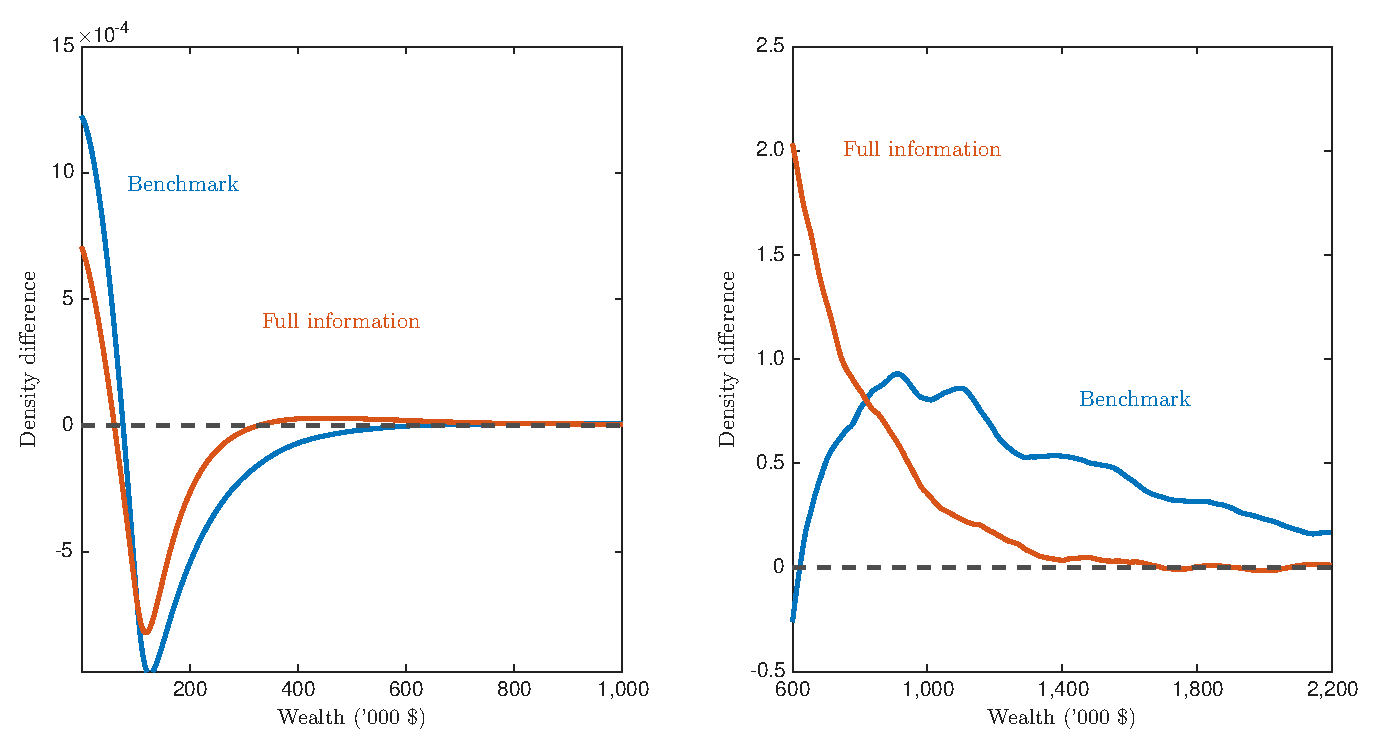
\includegraphics[viewport=-40bp -2bp 900bp 355bp,clip,scale=0.65]{_input/figure_d1}
\par\end{centering}
{\footnotesize\emph{Note}}{\footnotesize : The figure shows changes
in the average wealth distribution in response to an increase in the
replacement rate by 10 percentage points.. We illustrate these changes
for both our calibrated model (``Benchmark Model'') and the associated
full-information economy (``Full Information''). We use 2020 values
of U.S. household income to convert capital-holdings in the model
to \$ amounts. Probability density functions are estimated from a
simulated panel of households, using a kernel density estimator with
the Epanechnikov kernel.}{\footnotesize\par}
\end{figure}

\enlargethispage{\baselineskip}
\begin{table}[H]
\caption{Extended Model: Effects of Increased Unemployment Benefits}

\textcolor{black}{\label{app-tab:extended-model-ui}\vspace{-0.29cm}}

\begin{centering}

\textcolor{black}{\def\sym#1{\ifmmode^{#1}\else\(^{#1}\)\fi}

\begin{tabular}{lcccccc}
\toprule
\toprule
                  & $\mu(K)$ & $\sigma(Y)$ & $\text{Gini}(K)$ & $90/50$  & Info U. & Info E.\\
\midrule
Endogenous Information & -2.05 & 2.95 & 7.42 & 39.21 & -21.36 & -4.66\\ 
[1em] Exogenous Information & -1.27 & 0.70 & 3.82 & 15.57 & . & .\\ 
[1em] Full Information & -1.21 & 0.28 & 2.82 & 11.05 & . & .\\ 
\bottomrule
\bottomrule
\end{tabular}
}

\end{centering}

\vspace{0.38cm}

{\footnotesize\emph{Note}}{\footnotesize : The table shows the effects
of a ten percentage-point increase in the replacement rate on moments
of the average cross-sectional capital distribution and the logarithm
of economy-wide output in percent. $\mu(K)$ denotes the mean of the
)capital stock, while $\sigma(Y)$ denotes the standard deviation
of (log-)economy-wide output. The table computes the moments for the
both benchmark economy (``Benchmark Model'') and the associated
full-information and exogenous-information economies (``Full Information''
and ``Exogenous Information'', respectively). The final two columns
measure the percent difference in the average number of households
who acquire information. We compute this probability separately for
the employed and unemployed.}{\footnotesize\par}
\end{table}

\end{document}
